%==============================================================================
% tento soubor pouzijte jako zaklad
% this file should be used as a base for the thesis
% Autoři / Authors: 2008 Michal Bidlo, 2019 Jaroslav Dytrych
% Kontakt pro dotazy a připomínky: sablona@fit.vutbr.cz
% Contact for questions and comments: sablona@fit.vutbr.cz
%==============================================================================
% kodovani: UTF-8 (zmena prikazem iconv, recode nebo cstocs)
% encoding: UTF-8 (you can change it by command iconv, recode or cstocs)
%------------------------------------------------------------------------------
% zpracování / processing: make, make pdf, make clean
%==============================================================================
% Soubory, které je nutné upravit nebo smazat: / Files which have to be edited or deleted:
%   projekt-20-literatura-bibliography.bib - literatura / bibliography
%   projekt-01-kapitoly-chapters.tex - obsah práce / the thesis content
%   projekt-01-kapitoly-chapters-en.tex - obsah práce v angličtině / the thesis content in English
%   projekt-30-prilohy-appendices.tex - přílohy / appendices
%   projekt-30-prilohy-appendices-en.tex - přílohy v angličtině / appendices in English
%==============================================================================
%\documentclass[slovak]{fitthesis} % bez zadání - pro začátek práce, aby nebyl problém s překladem
%\documentclass[english]{fitthesis} % without assignment - for the work start to avoid compilation problem
%\documentclass[zadani]{fitthesis} % odevzdani do wisu a/nebo tisk s barevnými odkazy - odkazy jsou barevné
\documentclass[slovak,zadani]{fitthesis} % for submission to the IS FIT and/or print with color links - links are color
%\documentclass[zadani,print]{fitthesis} % pro černobílý tisk - odkazy jsou černé
%\documentclass[english,zadani,print]{fitthesis} % for the black and white print - links are black
%\documentclass[zadani,cprint]{fitthesis} % pro barevný tisk - odkazy jsou černé, znak VUT barevný
%\documentclass[english,zadani,cprint]{fitthesis} % for the print - links are black, logo is color
% * Je-li práce psaná v anglickém jazyce, je zapotřebí u třídy použít 
%   parametr english následovně:
%   If thesis is written in English, it is necessary to use 
%   parameter english as follows:
%      \documentclass[english]{fitthesis}
% * Je-li práce psaná ve slovenském jazyce, je zapotřebí u třídy použít 
%   parametr slovak následovně:
%   If the work is written in the Slovak language, it is necessary 
%   to use parameter slovak as follows:
%      \documentclass[slovak]{fitthesis}
% * Je-li práce psaná v anglickém jazyce se slovenským abstraktem apod., 
%   je zapotřebí u třídy použít parametry english a enslovak následovně:
%   If the work is written in English with the Slovak abstract, etc., 
%   it is necessary to use parameters english and enslovak as follows:
%      \documentclass[english,enslovak]{fitthesis}

% Základní balíčky jsou dole v souboru šablony fitthesis.cls
% Basic packages are at the bottom of template file fitthesis.cls
% zde můžeme vložit vlastní balíčky / you can place own packages here

% Kompilace po částech (rychlejší, ale v náhledu nemusí být vše aktuální)
% Compilation piecewise (faster, but not all parts in preview will be up-to-date)
% \usepackage{subfiles}

% Nastavení cesty k obrázkům
% Setting of a path to the pictures
%\graphicspath{{obrazky-figures/}{./obrazky-figures/}}
%\graphicspath{{obrazky-figures/}{../obrazky-figures/}}

%---rm---------------
\renewcommand{\rmdefault}{lmr}%zavede Latin Modern Roman jako rm / set Latin Modern Roman as rm
%---sf---------------
\renewcommand{\sfdefault}{qhv}%zavede TeX Gyre Heros jako sf
%---tt------------
\renewcommand{\ttdefault}{lmtt}% zavede Latin Modern tt jako tt

% vypne funkci šablony, která automaticky nahrazuje uvozovky,
% aby nebyly prováděny nevhodné náhrady v popisech API apod.
% disables function of the template which replaces quotation marks
% to avoid unnecessary replacements in the API descriptions etc.
\csdoublequotesoff



\usepackage{url}


% =======================================================================
% balíček "hyperref" vytváří klikací odkazy v pdf, pokud tedy použijeme pdflatex
% problém je, že balíček hyperref musí být uveden jako poslední, takže nemůže
% být v šabloně
% "hyperref" package create clickable links in pdf if you are using pdflatex.
% Problem is that this package have to be introduced as the last one so it 
% can not be placed in the template file.
\ifWis
\ifx\pdfoutput\undefined % nejedeme pod pdflatexem / we are not using pdflatex
\else
  \usepackage{color}
  \usepackage[unicode,colorlinks,hyperindex,plainpages=false,pdftex]{hyperref}
  \definecolor{hrcolor-ref}{RGB}{223,52,30}
  \definecolor{hrcolor-cite}{HTML}{2F8F00}
  \definecolor{hrcolor-urls}{HTML}{092EAB}
  \hypersetup{
	linkcolor=hrcolor-ref,
	citecolor=hrcolor-cite,
	filecolor=magenta,
	urlcolor=hrcolor-urls
  }
  \def\pdfBorderAttrs{/Border [0 0 0] }  % bez okrajů kolem odkazů / without margins around links
  \pdfcompresslevel=9
\fi
\else % pro tisk budou odkazy, na které se dá klikat, černé / for the print clickable links will be black
\ifx\pdfoutput\undefined % nejedeme pod pdflatexem / we are not using pdflatex
\else
  \usepackage{color}
  \usepackage[unicode,colorlinks,hyperindex,plainpages=false,pdftex,urlcolor=black,linkcolor=black,citecolor=black]{hyperref}
  \definecolor{links}{rgb}{0,0,0}
  \definecolor{anchors}{rgb}{0,0,0}
  \def\AnchorColor{anchors}
  \def\LinkColor{links}
  \def\pdfBorderAttrs{/Border [0 0 0] } % bez okrajů kolem odkazů / without margins around links
  \pdfcompresslevel=9
\fi
\fi
% Řešení problému, kdy klikací odkazy na obrázky vedou za obrázek
% This solves the problems with links which leads after the picture
\usepackage[all]{hypcap}

% Informace o práci/projektu / Information about the thesis
%---------------------------------------------------------------------------
\projectinfo{
  %Prace / Thesis
  project={BP},            %typ práce BP/SP/DP/DR  / thesis type (SP = term project)
  year={2022},             % rok odevzdání / year of submission
  date={11.5.2022},             % datum odevzdání / submission date
  %Nazev prace / thesis title
  title.cs={Generování rodokmenů z matričních záznamů},  % název práce v češtině či slovenštině (dle zadání) / thesis title in czech language (according to assignment)
  title.en={Family Trees Making from Parish Records}, % název práce v angličtině / thesis title in english
  %title.length={14.5cm}, % nastavení délky bloku s titulkem pro úpravu zalomení řádku (lze definovat zde nebo níže) / setting the length of a block with a thesis title for adjusting a line break (can be defined here or below)
  %sectitle.length={14.5cm}, % nastavení délky bloku s druhým titulkem pro úpravu zalomení řádku (lze definovat zde nebo níže) / setting the length of a block with a second thesis title for adjusting a line break (can be defined here or below)
  %dectitle.length={14.5cm}, % nastavení délky bloku s titulkem nad prohlášením pro úpravu zalomení řádku (lze definovat zde nebo níže) / setting the length of a block with a thesis title above declaration for adjusting a line break (can be defined here or below)
  %Autor / Author
  author.name={Adam},   % jméno autora / author name
  author.surname={Marhefka},   % příjmení autora / author surname 
  %author.title.p={Bc.}, % titul před jménem (nepovinné) / title before the name (optional)
  %author.title.a={Ph.D.}, % titul za jménem (nepovinné) / title after the name (optional)
  %Ustav / Department
  department={UITS}, % doplňte příslušnou zkratku dle ústavu na zadání: UPSY/UIFS/UITS/UPGM / fill in appropriate abbreviation of the department according to assignment: UPSY/UIFS/UITS/UPGM
  % Školitel / supervisor
  supervisor.name={Jaroslav},   % jméno školitele / supervisor name 
  supervisor.surname={Rozman},   % příjmení školitele / supervisor surname
  supervisor.title.p={Ing.},   %titul před jménem (nepovinné) / title before the name (optional)
  supervisor.title.a={Ph.D.},    %titul za jménem (nepovinné) / title after the name (optional)
  % Klíčová slova / keywords
  keywords.cs={genealógia, grafová databáza, matričné záznamy, spracovávanie záznamov}, % klíčová slova v českém či slovenském jazyce / keywords in czech or slovak language
  keywords.en={genealogy, graph database, parish records, record processing}, % klíčová slova v anglickém jazyce / keywords in english
  %keywords.en={Here, individual keywords separated by commas will be written in English.},
  % Abstrakt / Abstract
  abstract.cs={Práca sa zaoberá oborom genealógie, spracovávaním, porovnávaním a klasifikovaním
genealogických dát a následným prepájaním týchto dát do väčších celkov v grafovej 
databáze. Táto práca priamo nadväzuje na prácu Ing. Tušimovej a ďalej ju rozširuje. 
Rozšírenia popísané v práci sa budú týkať pridania podpory pre ďalšie formy vstupných 
genealogických dát, optimalizácií a vylepšení hlavného algoritmu realizujúceho 
spracovávanie genealogických záznamov. Cieľom práce bude teda zefektívniť algoritmus, 
zvýšiť jeho presnosť a pridať podporu pre matriky sobášov a úmrtí.}, % abstrakt v českém či slovenském jazyce / abstract in czech or slovak language
  abstract.en={This work will discuss the field of genealogy, processing, comparing, and classifying 
genealogical data and subsequent connection of this processed data into bigger structures in 
graph database. This work directly continues the work of Ing Tušimová and further expands it. The expansions described in the work will be dedicated to addition of support for 
more forms of input genealogical data, optimization and expansions of the core algorithm 
realizing the processing of genealogical records. The goal of this work is therefore to make 
the core algorithm more efficient and precise as well as the addition of support for parish 
records of marriages and deaths.}, % abstrakt v anglickém jazyce / abstract in english
  %abstract.en={An abstract of the work in English will be written in this paragraph.},
  % Prohlášení (u anglicky psané práce anglicky, u slovensky psané práce slovensky) / Declaration (for thesis in english should be in english)
  declaration={Prehlasujem, že som túto bakalársku prácu vypracoval samostatne pod vedením pána Ing. Jaroslava Rozmana Ph.D.. Uviedol som všetky literárne pramene, publikácie a ďalšie zdroje, z ktorých som čerpal.},
  %declaration={I hereby declare that this Bachelor's thesis was prepared as an original work by the author under the supervision of Mr. X
% The supplementary information was provided by Mr. Y
% I have listed all the literary sources, publications and other sources, which were used during the preparation of this thesis.},
  % Poděkování (nepovinné, nejlépe v jazyce práce) / Acknowledgement (optional, ideally in the language of the thesis)
  acknowledgment={Ďakujem vedúcemu mojej práce, Ing. Jaroslavovi Rozmanovi Ph.D. za jeho ochotu a odbornú pomoc pri vypracovávaní tejto bakalárskej práce.},
  %acknowledgment={Here it is possible to express thanks to the supervisor and to the people which provided professional help
%(external submitter, consultant, etc.).},
  % Rozšířený abstrakt (cca 3 normostrany) - lze definovat zde nebo níže / Extended abstract (approximately 3 standard pages) - can be defined here or below
  %extendedabstract={Do tohoto odstavce bude zapsán rozšířený výtah (abstrakt) práce v českém (slovenském) jazyce.},
  %extabstract.odd={true}, % Začít rozšířený abstrakt na liché stránce? / Should extended abstract start on the odd page?
  %faculty={FIT}, % FIT/FEKT/FSI/FA/FCH/FP/FAST/FAVU/USI/DEF
  faculty.cs={Fakulta informačních technologií}, % Fakulta v češtině - pro využití této položky výše zvolte fakultu DEF / Faculty in Czech - for use of this entry select DEF above
  faculty.en={Faculty of Information Technology}, % Fakulta v angličtině - pro využití této položky výše zvolte fakultu DEF / Faculty in English - for use of this entry select DEF above
}

% Rozšířený abstrakt (cca 3 normostrany) - lze definovat zde nebo výše / Extended abstract (approximately 3 standard pages) - can be defined here or above
%\extendedabstract{Do tohoto odstavce bude zapsán výtah (abstrakt) práce v českém (slovenském) jazyce.}
% Začít rozšířený abstrakt na liché stránce? / Should extended abstract start on the odd page?
%\extabstractodd{true}

% nastavení délky bloku s titulkem pro úpravu zalomení řádku - lze definovat zde nebo výše / setting the length of a block with a thesis title for adjusting a line break - can be defined here or above
%\titlelength{14.5cm}
% nastavení délky bloku s druhým titulkem pro úpravu zalomení řádku - lze definovat zde nebo výše / setting the length of a block with a second thesis title for adjusting a line break - can be defined here or above
%\sectitlelength{14.5cm}
% nastavení délky bloku s titulkem nad prohlášením pro úpravu zalomení řádku - lze definovat zde nebo výše / setting the length of a block with a thesis title above declaration for adjusting a line break - can be defined here or above
%\dectitlelength{14.5cm}

% řeší první/poslední řádek odstavce na předchozí/následující stránce
% solves first/last row of the paragraph on the previous/next page
\clubpenalty=10000
\widowpenalty=10000

% checklist
\newlist{checklist}{itemize}{1}
\setlist[checklist]{label=$\square$}

% Nechcete-li, aby se u oboustranného tisku roztahovaly mezery pro zaplnění stránky, odkomentujte následující řádek / If you do not want enlarged spacing for filling of the pages in case of duplex printing, uncomment the following line
% \raggedbottom
\usepackage{pdfpages}
\usepackage{multicol}
\usepackage{fixltx2e}
\begin{document}
  
  % Vysazeni titulnich stran / Typesetting of the title pages
  % ----------------------------------------------
  \maketitle
  
  % Obsah
  % ----------------------------------------------
  \setlength{\parskip}{0pt}
  
  {\hypersetup{hidelinks}\tableofcontents}
  
  % Seznam obrazku a tabulek (pokud prace obsahuje velke mnozstvi obrazku, tak se to hodi)
  % List of figures and list of tables (if the thesis contains a lot of pictures, it is good)
  \ifczech
    \renewcommand\listfigurename{Seznam obrázků}
  \fi
  \ifslovak
    \renewcommand\listfigurename{Zoznam obrázkov}
  \fi
  % {\hypersetup{hidelinks}\listoffigures}
  
  \ifczech
    \renewcommand\listtablename{Seznam tabulek}
  \fi
  \ifslovak
    \renewcommand\listtablename{Zoznam tabuliek}
  \fi
  % {\hypersetup{hidelinks}\listoftables}

  \ifODSAZ
    \setlength{\parskip}{0.5\bigskipamount}
  \else
    \setlength{\parskip}{0pt}
  \fi

  % vynechani stranky v oboustrannem rezimu
  % Skip the page in the two-sided mode
  \iftwoside
    \cleardoublepage
  \fi

  % Text prace / Thesis text
  % ----------------------------------------------
  \ifenglish
    % This file should be replaced with your file with an thesis content.
%=========================================================================
% Authors: Michal Bidlo, Bohuslav Křena, Jaroslav Dytrych, Petr Veigend and Adam Herout 2019

\chapter{Introduction}

This text serves as example content of this template and as a recap of the most important information from regulations, it also provides additional useful information, that you will need when you write a technical report for your academic work. Check out appendix \ref{jak} before you use this template as it contains vital information on how to use it.

Even though some students only need to know and comply with the official formal requirements stated in regulations as well as typographical principles to write a good diploma thesis (bachelor's thesis is a diploma thesis too -- you get a diploma for it), it is never a~bad idea to familiarize yourself with some of the well-established procedures for writing a~technical text and make things easier for yourself. Some supervisors had prepared breakdowns of proven procedures that have lead to tens of successfully presented academic works. A~selection of the most interesting procedures available to the authors of this work at the time of writing can be found in chaptes below. If your supervisor has their own web page with recommended procedures, you can skip these chapters and follow their instructions instead. If that is not the case, you should read the respective chapters proir to consulting your supervisor about the structure and contents of your academic work.

Diploma thesis is an extensive work and the technical report should reflect it. It is not easy for everyone to sit down and simply write it. You need to know where to begin and how to progress. One of many viable approaches is to start with keywords and abstract, this helps you establish what the most important part of your work is. More on that in~chapter~\ref{abstrakt}.

Once the abstract is finished, you can start with the text of the technical report. The first thing you should do is create a structure for your work, that you'll later fill with text. Chapter \ref{struktura} provides basic information and hints on writing a technical text, that can help you avoid mistakes beginners make, create chapter titles and figure out what the approximate length of individual chapters should be. The chapter concludes with an approach that should make writing a thesis much easier.

Diploma theses in the field of information technology have a specific  structure. The introduction is followed by a chapter or chapters dealing with the summary of the current state. The next chapter should evaluate the current state and provide a solution, that will be implemented and tested. The conclusion should contain evaluated results and ideas for future development. Even though the chapter titles and their length may differ from other theses, you can always find chapters that correspond with this structure. Chapter \ref{kapitoly} deals with the contents of chapters that commonly occur in dimploma theses in the field of information technology. Most students will only use a subset of all the described chapters as not everything will be relevant for their thesis. The descriptions and hints provided help students with the inner structure and the contents of chapters as well as decide whether or they should even include given chapter. 

The final chapter of a thesis is always followed by a list of references. Citations that this list is comprised of and their respective links is the subject of chapter \ref{citace}. An inexperienced student may not perceive it that way, but the list of references is a vital part of a thesis. One of the important aspects of your reviewer's evaluation is how you work with literature. A single missing entry can lead to an F for your grade, disciplinary proceedings for plagiarism and ultimately to being expelled. There are other consequences to this as two czech ministers resigned over allegations of plagiarism in 2018. Be as thorough as possible in creating your list of references.

When you're done with the text, it is necessary to figure out what the requirements for a thesis at BUT FIT are and work the kinks out. Formal requirements that are stated in~regulations and at faculty web pages can be found in chapter \ref{formality}. This chapter also contains information about the required length of different types of academic works and other helpful information. The chapter concludes with an overview of the most common mistakes that the reviewers have to deal with and that you should avoid. The review of the formal aspect of thesis is just another important part of the reviewer's assessment.

Once you deal with the formal deficiencies, you can sumbit your thesis. Before you do so, go through the checklist in appendix \ref{checklist}. The submission of paper and electronic versions of a thesis is described in chapter \ref{odevzdani}.

Chapter \ref{zaver} contains a summary of what you can learn by reading this text, and most importantly things to keep in mind before you submit your thesis.

\chapter{Abstract}
\label{abstrakt}

Ther should be a summary of work at most 10 lines long under the Abstract heading. Despite how short it is, a good abstract provides enough information to know what the problem is, what was the chosen solution as well as the results achieved. The purpose of abstract is to let the reader know whether or not they can find the answer to their question here. The rest of this chapter was taken from professor Herout's blog \cite{Herout}.
\bigskip

\noindent First and foremost - abstract matters. Second - It's not that hard to write one. Without further ado, let's dive into it.

\subsection*{What is the purpose of an abstract}
An abstract is used for \bf searching \rm purposes, together with the title of thesis and a list of keywords. These parts (perhaps except for the title) are not directly part of the text and it's not expected that anyone who will read your thesis actually reads them. The fact that they're reading your thesis means they're past the abstract stage. Abstract serves them well to decide \bf whether or not \rm they want to read your thesis.

When someone looks for an answer to their problem, they give the librarian or a search engine (these days) keywords that directly relate to their problem. They then receive list of theses, that could possibly offer a solution based on the match between the keywords used and keywords in the theses. A good thesis title can help the person guess which texts could have a direct relation with their problem and can get them to read your thesis.

This is where abstract is crucial. The reader reads abstracts of the theses and decides, whether or not they want to read them. It also informs the them that their filter based on a title alone is wrong.

At this point, they don't have a PDF with full text or a printed version of the thesis available. Abstracts are \bf not \rm supposed to be in the text itself, but to be available on servers aggregating scientific texts. Therefore the first rule is: an abstract needs to work on it's own -- if it contains references to literature or text (``The efficiency of a method is summarized on page 51.''), it only makes a reader less interested in the author, won't read their work or cite them.


\subsection*{When and how to write an abstract}
It makes the sense to write an abstract when the writing is done -- as a summary and real annotation of the thesis.
I however like the opposite approach -- write an abstract in the beginning. Whenever I write a scientific article, I start with a long list of keywords that are related to eachother. It's a lot more than end up as the final keywords used for indexing. It help me understand where the article is headed at all times -- what should I talk about, what needs to be in the text, what does it deal with. As soon as I'm done with keywords, I form a title and an abstract.

I consider the following four parts of an abstract especially useful -- Which problem does it solve? What solution does it offer? What are the results? What is the meaning of these results? Once all of this is clear, the text essentially writes itself. If this is unclear, how on earth can you form a coherent, meaningful sentence in the same text?


\subsection*{Recommended structure of the abstract}
An abstract of a scientific thesis can consist of four parts and be useful. Each individual part consists of two to three sentences, in some cases even a single sentence is enough.

The term ``elevator pitch'' is often used in bussiness. It is not a coincidence that its structure is similar to the recommended structure of an abstract. Realistically, an abstract should contain anything the author would say about their scientific thesis if they had at most 2 minute and could not use slides, images or text. What should they talk about then?

\paragraph{Part one -- What is the problem? What is the topic? What's the goal of the text?}
\begin{itemize}
  \item{This thesis deals with.}
  \item{The goal of this thesis is.}
  \item{My aim was.}
\end{itemize}
There is no place for fairy tales specific to wrong scientific literature: ``Our five-year-plan of~work open new and bold goals for us'', ``With the evolution of computing technology and especially the display devices, it is more important than ever \ldots'' do not belong anywhere near a good text, especially an abstract. If you can express the purpose of your text in one sentence, do it and forget about everything else. Less is always more when it comes to the abstract.

\paragraph{Part two -- How is the problem solved? Is the goal fulfilled?}
\begin{itemize}
  \item{I solved the problem using this and that.}
  \item{I used this method, this procedure and analysed this.}
  \item{The work represents an algorithm that.}
  \item{I used these tools to process data and evaluated results like this.}
  \item{The principle of our algorithm is.}
\end{itemize}

There is a new methodology in the nature of scientific text (= ``how to do something''), it needs to include a description. If the solution consists of three parts, it probably means that this part of an abstract will have three sentences, where each sentence is about a~different part of the solution. A good abstract is be honest and accurate in this section -- no ``revealing secrets'' in the text itself. Vague formulations of a solution principle in~an~abstract usually means that the authors can't write or don't have anything to write about -- neither one is good enough to waste your time.

\paragraph{Part three -- What are the results? How good is the solution?}
\begin{itemize}
  \item{It was 87,3\,\% successful.}
  \item{We created a system that.}
  \item{The solution offers these options.}
  \item{As a result, we found out that.}
\end{itemize}

Stating a specific number is not a bad habit in this part -- ``we made existing XY method five times faster''. If the contributon of your work cannot be summarized in two or three sentences, something is wrong and the entire text is probably not worth writing.

\paragraph{Part four -- Well then? What does it bring to science and the reader?}
\begin{itemize}
  \item{The contribution of this thesis is.}
  \item{The primary discovery is.}
  \item{The primary result is.}
  \item{Based on the data it is possible to.}
  \item{The results allow us to.}
\end{itemize}

When writing scientific articles, I myself struggle with the similarity of third and fourth part. Both of them speak about the results and contribution of the text. The goal of the third part is to be specific and name achieved results whereas the goal of the fourth part is to interpret their meaning and significance. I guess it's fine if these two statements merge to an extent and both parts not only don't have their own paragraph, but they sometimes even intertwine with their common sentences.

\paragraph{Part zero -- What is it about? Where are we?}
\begin{itemize}
  \item{The context is this and this.}
  \item{It deals with studies of this and that.}
  \item{We build on these recent advances in our field.}
\end{itemize}

Sometimes it is necessary to insert a short specification of context at the beginning of your abstract. It can be a great asset when it comes to obscure and esoteric field, that is off to the side of the main flow. Usually this part is not needed and sentences contained here are prime examples for pseudoscientific nonsense. It's not necessarily bad to forget that this part can even exist in an abstract. If an expert in the field shakes their head after reading an abstract: ``I have no idea what this is about.'' only then it makes sense to include this part to specify context.


\subsection*{Innovation is not ignorance}

In this text I describe a general model of a general thesis. I would like to state that this is my opinion and taste and I'm interested in alternate opinions and tastes (I really am!). Every graduate (Mgr. and Bc.) feels that their thesis is special and extraordinary. Therefore they won't follow some scheme meant for common and average theses -- i.e. the others. I see good reasons to divert from the outlined scheme and recommend some students to divert from the scheme myself every year. Indeed, every thesis is unique and extraordinary. If they weren't, there would be no reason to write them, just copy them instead. Before you divert from the standard and canonical way of organizing scientific text, put some effort into learning, understanding and tackling it. The way of scientific work, structuring scientific text or citing sources can look rigid and clumsy, but for now it is the best way mankind could come up with. If you learn it, understand it's advantages and disadvantages and innovate it, it's great and you're welcome to do so. If you choose to ignore it, you'll most likely end up with a very poor innovation.

\chapter{Drafting the basic thesis structure}
\label{struktura}

This chapter contains a selection of useful hints and procedures useful for writing a dissertation (bachelor's thesis is technically a dissertation -- you receive a diploma for it) from experienced supervisors. First a number of general princples are listed, followed by a more detailed description of the advised procedure of drafting a thesis structure.

Before you into it head first, ask your supervisor for any advices or if they have their own web page with hints and guidelines. Their area of expertise will probably coincide with that of your thesis and help you with the most appropriate structure that you should comply with. If the authors learn about a another collection of useful hints, you'll find it here in the future.

This text deals with the general recommendations and thesis structure, that always has to be modified and thought of based on the specification \cite{Cernocky}.


\section{Useful hints for writing a technical text}

The following instructions can also be found on faculty web pages\cite{fitWeb}. The overview of basic typography and the creation of documents using \LaTeX{} system can be found in Jiří Rybička's book\cite{Rybicka}.

One of the evaluated parts of a potential engineer is quality of language and literacy. Your goal is to create a clear and comprehensive text. You should express yourself accurately, use the appropriate level of Czech or Slovak grammar (or English if need be) and comply with the generally accepted customs. Slang words and phrases are not allowed. If you are uncertain of the translation or transcription of foreign terms, use literature available in FIT library.

The text should be a short path to understanding a problem, predict it's difficulties and preventing them. Good writing means perfect grammar, correct punctuation and use of appropriate words. You should strive for a good text, one that is not monotonous due to use of small selection of words, or overuse of some of your favorite words. If you use foreign words, it is expected that you know their exact meaning. Obviously, you need to use english words correctly as well. For example, there are certain rules when using the word {\it obvious}. Is {\it obvious} really obvious? And did you make sure, that the {\it obvious} is really valid? You should be careful about using the subject {\it it} with a passife voice too often. For example, you should never use the Czech {\it it has proved itself that...}, ever.

It is advised to think the use of symbols for {\it labelling} through thoroughly. By this we mean a well thought out choice of abbreviations and symbols used for distinguishing types of parts, labelling program's main functions, naming control keys on keyboard, naming variables in math formulas etc. Apt and consistent labelling can help reader a lot. It is advised to provide a list of labelling at the beginning of text. Not just in labelling, consistency is important in references and in typesetting in general.

There are numerous typographical principles that can be used to distinguish things. You can choose different styles for different purposes. As an example, keys can be placed in a rectangle, identifiers from source text can be written in {\tt typewriter font} etc.

Whenever you state facts, you should also state their origin and your attitude to them. If you claim something, you always have to explicitly state, which part of it was proven, what will be proven in your text and what you took from literature (including it's source). You should never let the reader doubt whose idea they're presented with, your own or someone else's.


If you want to write a clear and comprehensive academic text, you need follow these rules:
\begin{itemize}
\item You must have something to say,
\item you must know, who you want to say it to,
\item you must thoroughly think through the contents,
\item you must write in a structured way 
\end{itemize}

\subsection*{You must have something to say}
The most important prerequisite of a good academic text is to have an idea. If the idea is significant enough, it will last, even if it is not formulated in the best way. However, if you want to articulate your idea as precisely as possible and save the reader's time, you must comply with certain principles discussed further below.

\subsection*{You must know, who you want to say it to}
Another imporant prerequisite of a good academic text is the audience. If you write down notes for yourself, you usually write in a differently than when you write a scientific report, article, thesis, book or a letter. Depending on who the target audience is, you can decide the writing style, the amount of information and how detailed it is. 

\subsection*{You must thoroughly think through the contents}
You must thoroughly think through the contents of your thesis as well as the order in which you want to present the reader with your ideas. As soon as you know what you want to say and to whom, you need to create a structure. The ideal structure should be one that is logically accurate and psychologically digestible, where everything has it's place and it's individual parts fit into each other. All the conncetions between them are clear and it's apparently what belongs where.

To achieve this goal, you must precisely structure the contents of your text. Decide what the main chapters and subchapters are going to be, as well as the connection between them. A diagram of such structure would be a tree-like graph, not a chain. When structuring the contents, it is important to ask yourself what you want to include as well as what you want to exclude. Too much detail could discourage the reader, and so could lack of detail.

The result of this stage is an outline of the text consisting of the main ideas and all the details between connecting them to eachother.

\subsection*{You must write in a structured way}

You must write in a structured way and work the most comprehensible format simultaneously, good writing and perfect labelling included. If you have an idea, you know who your target audience is, you know your goal and outline of the text, then you're ready to start writing. When writing your initial draft, you should try to include all your ideas and opinions regarding the individual chapters and subchapters. You need to explain every single idea, describe and prove. The main idea should always be formulated in a main clause, rather than the dependant clause.

You should approach the writing itself in a structured way too. As you're working on the structure of your thesis, you're creating a framework that you are gradually completing. You should use a DPT\footnote{Desktop publishing (DTP) - creating printed document on a computer.} program that offers a structured layout of text (pre-defined types of headings and text blocks).

\subsection*{It will never be perfect}
Once you have written everything you thought about, you should take a day or two off, then read what you wrote again. Make last changes and move on. You should know that something will always remain unfinished, and that there is always a better way of explaining something, but every stage of the editing must come to an end.

\section{Who is the target audience of a thesis}

This subsection was taken from professor Herout's blog \cite{Herout}.

\bigskip
\noindent \bf Write your thesis for a student, that will build on your work. \rm
\bigskip

Imagine that another student will continue the work in your thesis, they're about as~smart as you are. You have four hours to show them your thesis, explain everything necessary for them to be able to continue your work. The student studies at the same school and knows about as much as an average student would, they're not an expert in the area of your thesis, but they're not stupid either. The student just found out that they'll continue your work, so they had no time to learn about the topic, just like you.

It's best to start by telling the student what the goal of this thesis is and what the results should look like.

Nobody in their right mind will spend an hour explaining things like this to the student: ``{\mbox{Interet} was invented by the american army in 1962, then www was invented in CERN in 1991, nowadays it is used for various purposes.''}(all of this on six pages with countless references and figures).
The student usually doesn't need countless pages of details regarding colorful modules to represent figures, history and details of Hough transformation, complete description of the ISO/OSI reference model layers or a set of pie graphs representing individual mobile platforms on the market over the last decade.
The student needs to be shown the valuable sources that helped you and wants a brief description of tools and algorithms that were a vital part of the solution: ``{You need XY tool that does this and that, especially it's PQ module, that is used then and then. The most useful information can be found in~this documentation.}''

Tell the student everything about what worked for you and what helped, but also make sure to tell them what seemed like a good idea, but ended up being useless.

Try to provide just the right amount of detail. Explain an optimization method one line of code at a time, a module in one paragraph enriched with description of input and output data, and a reference to the respective library.

Imagine this four hours long session with the student.
\begin{itemize}
  \item{What do you think you would talk about in the beginning, how long did it take for the student to understand?}
  \item{What are some things that should be mentioned?}
  \item{What kind of figures would you draw during the session?}
  \item{What would the student ask about, what is important but not clear?}
  \item{What restrictions and unfinished things would you need to inform the student about to prevent them from falling into a trap?}
  \item{How can the student continue? What is left unfinished and is worth trying? What could be improved?}
  \item{What would you say in the very first and very last minute of the session?}
\end{itemize}


\section{Thesis structure -- Five chapters}

This subsection was taken from the blog of professor Herout\cite{Herout} (partially inspired by a book from Jean-Luc Lebrun \cite{Lebrun2011}) and from a document on professor Zemčík's web page \cite{Zemcik}.
\bigskip

Thesis is something that students work on for 2 semesters of their studies and then write a small book about it. The misconception is that this little book is the master's thesis. The book is in fact a technical report about the year long work and master's thesis represents the result of student's work.

The year long work includes studies first and foremost: ``What already exists in the area of my thesis? How did the others do it?'' It is implied that a student tries to innovate and design some things: ``The problem has several solutions, I chose this approach, because it is the most efficient option for the given platform.''
The researcher should implement and evaluate their designs to validate them: ``I used these tools for implementation, the entire system is split into these modules. The result is this fast, it is this effective and user reviews are such and such.''

The basic structure of master's thesis according to professor Herout is as follows:
\begin{enumerate}
  \item{Introduction (1 page)}
  \item{What had to be studied (including assessment of the current state; 40\,\%)}
  \item{New ideas that this thesis explores (30\,\%)}
  \item{Implementation and evaluation (30\,\%)}
  \item{Conclusion (1 page)}
\end{enumerate}

If the text has these 5 chapters, it is not a mistake, neither is if one of them is split in two parts -- more on that later. A big mistake is when any of the parts are missing, or when it's content differs from the rest.

Names of chapters can vary from this structure, even though your thesis will have an introduction and a conclusion. The content of your thesis itself is what really matters and if it means you have to break the structure, then do so.

Many supervisors agree with this basic structure, even though some of the recommend different chapter titles and for example assessment of the current state can be used in second chapter, and even in third chapter according to professor Zemčík:
\begin{enumerate}
\item Introduction (1--2 pages)
\item Summary of the current state (40--50\,\%)
\item Assesment of the current state and solution draft (3-5 pages)
\item Your own work (roughly 40\,\%)
\item Conclusion (at most 1 page)
\end{enumerate}

Opinions of supervisors also differ in length depending on the specification of thesis, this can be seen for example in recommendations from assistant professor Beran \cite{Beran}:
\begin{enumerate}
\item Introduction (1 page)
\item Theory (1/3 of pages)
\item Solution draft (1/3 of pages)
\item Implementation, experiments and assessment (1/3 of pages)
\item Conclusion (1 page)
\end{enumerate}

When it comes to practice-oriented theses, where the most important things are data and user interface, associate professor Černocký \cite{Cernocky} recommends the following:
\begin{enumerate}
\item Introduction (single digit of pages)
\item Theoretical part (roughly 10 pages)
\item Data (single digit of pages)
\item Breakdown of Your algorithm and testing (roughly 10 pages)
\item Draft and implementation (several pages)
\item User interface (several pages)
\item Testing (roughly 10 pages)
\item Conclusion (single digit of pages)
\end{enumerate}

\section{Thesis -- comics edition}

This subsection was taken from professor Herout's blog. \cite{Herout}.

Thesis (including bachelor's) is a fairly complex work comprised of a large amount of letters. These letters follow a certain hierarchy, organised into chapters. The whole thing should follow a logical order -- reader should first learn one thing so that they can then learn and understand other things. It should contain figures, tables, formulas; these non-textual objects should fit in with the surrounding text and enrich it. Every single aspect of the specification of your thesis has to be explored, it has to be finished by a certain date, printed and bundled into a book. If you want your thesis to be good, you need to make it good. Whenever you bake a cake from ten ingredients and one of them is rotten, it doesn't matter how hard you try, the cake will not taste good.

\subsection*{How should you approach everything?}

Whenever we write an article (all the time lately), we create something called a ``Comics Edition'' in the early stage. We do it because I insist that we do it and because it helps us a lot. Perhaps it can help you with your thesis.

First, make sure you know answers to the following questions:
\begin{itemize}
  \item{How would you explain the principle of your solution in three to five short sentences?}
  \item{What are the strenghts of your solution?}
  \item{What arguments would you use to support the correctness of your solution?}
  \item{If someone wanted to criticize your thesis -- what would they criticize it for?}
  \item{What would your answer be?}
  \item{What keywords should one use in a search engine to find your thesis in the search results?}
\end{itemize}

If you are finished, let's get into it...

\subsection*{Create THE document}

I often see people write an ``initial'' version of a thesis somewhere in their notes. First of all, that's extra work and second it is entirely pointless. It's best to create a document where the fight begins and also ends.

\subsection*{Chapter titles}

Chapter titles are an important part of a comics edition, put them in your document.

Put them in for the sake of formatting -- no provisional bullet point lists: ``I'll just do it later''. You need to see how the automatically generated content looks now, before it's too late to change everything.

Put them in for the sake of wording. Chapter title says, what the chapter is about. Chapter titles represent a skeleton covered in flesh and skin of text and figures.

Of all the words in your thesis, words in the titles are the \textbf most important ones\rm. Put some time and effort in your titles.

\subsection*{Figures}

Picture is worth a thousand words. I went through the last 8 articles that I helped write. They're 80 pages total and contain 87 figures and 17 tables, that's 1,3 of visual information per page (including pages containing references, title pages with abstracts etc). Many figures (about a half) are comprised of multiple subfigures, especially referenced figures. I~counted 221 of subfigures in the mentioned articles, that's an average of 3 visuals per page. This is what I imagine the role of figures in a scientific text should be. I think a~thesis with ``too many figures'' does not exist.

You should think about what images you will use and where they'll be even in the early stage of comics edition.

Figures don't have to be finished. We don't know what exactly the figure will represent just yet. We don't know what the caption will be. We only know that there will be a figure and that it will be comprised of multiple subfigures. It takes roughly a minute (we already have a vector format of a ``TODO Image'') and it shows us how the text will look.

In some cases, we know what the images will look like on a conceptual level. Draw it on a paper or a blackboard, take a picture of it and insert it where the final figure will be (vector image made in Inkscape\footnote{\url{https://inkscape.org}} or generated using Gnuplot\footnote{\url{http://www.gnuplot.info/}}). 

As a side note: Picture is worth a thousand words. Stupid picture is woth a thousand stupid words.

Just one more thing on the side when it comes to figures: If instead of vector images (schemes, graphs, drafts, diagrams, esentially everything except photos and screenshots) you use bitmap images and you use screenshots with a lossy compression (usually JPEG), don't expect a positive feedback or assessment.

\subsection*{Quantity of text}

Just like with figures we don't have yet, we insert even text that we don't have yet.

LaTeX has a beautiful command \textbackslash Blindtext\footnote{Short tutorial: \url{https://texblog.org/2011/02/26/generating-dummy-textblindtext-with-latex-for-testing/}} just for that. If you don't want to use it or don't know how, use \url{http://lipsum.com}. It helps you estimate the length of your work, figure density in text and other characterstics. It takes roughly 5 minutes to create this sort of estimate. To make sure you don't get lost in your work-in-progress text, change it's color to grey (smart person creates a command to change the color of the text unanimously for the whole document). From experience, it's easy to get lost without colors -- what is finished, what isn't and what needs to be worked on. It is advised to spend a couple minutes getting a text coloring package to work. You can use command \verb|\todo| in this template, for example \todo{This needs to be finished}.

The genesis of each chapter begins with 3-5 TODO pieces and some Lorem ipsum. Each TODO is then transformed into a larger number of TODOs of a smaller scale or into text, figure, other subchapters, and pretty much anything. TODOs come and go, but they always move you closer to the final product.

\subsection*{How do you work with it}

When you sit down and LaTeX is having a good day, it takes you an hour to write a thesis (bachelor's thesis included), with the right number of pages and a pretty good idea about where everything will be. It is slowly forming the result that is yet to come, after some more work.

The document does not really grow in size anymore, but it transforms. There's a~big difference between sitting down in front of a blank page and ``write a thesis'' and transforming one TODO into a paragraph. The first one is difficult and sometimes you just can't make it work. The latter works: it has it's head and tail. At least you know what to do.

Still, the thesis won't write itself, but it gets a lot easier and the final result is that much better.


\section{Chapter titles}

To publish well does not mean to fill up as many pages with letters as possible. Scientist's achieve their renown when their work is useful enough to another scientist, that they end up citing them. Therefore it is important that one's article is well written: nobody will cite a thesis that is poorly written because it degrades them.

Though poorly written article won't be cited because \bf nobody can find it\rm. Long before the internet SEO even existed, scientiests used all kinds of methods to make sure that other scientists working on their recherche will include others' materials that they read, make notes and finally -- cite in their work.

There are a lot of articles in the world. Whenever a scientist searches for materials relevant to their work, they enter keywords (formerly on paper in library, nowadys electronically into a search engine) and they get a lot of results -- e.g. titles. First step to get someone to cite an article is to have a good title. Title so good that a scientist is interested in your article enough to actually read it and find out more. Title is the \bf first filter\rm.


The scientist then opens the articles that satisfy the requirements of first filter. That means they get to see the abstract of the article. Abstract is the \bf second filter \rm and quite important one. It's similar to getting to a second round of interview for your dream job. People tend to care at that point.

If the scientist is interested in the title and the abstract, they download the entire PDF and scroll through quickly to get an idea: print it, or close the window and look for other articles? That is the \bf third filter \rm and it's similar to being among the last few dream job applicants. What are the scientist's interests in the third round? Visuals, i.e. figures, tables, formulas, and chapter titles. Does your article make it through the third filter? Will the scientist use your article? We'll talk about figures another time, this chapter is about titles after all.

It can be slightly different when it comes to theses. Not every author wants people to read their thesis. We belive that there are people who wish for the opposite. Let's just work with the hypothesis that the author wants to write a good text, that mankind could find useful and worth reading. One that gets a decent grade.


\subsection*{Keywords -- half the success}

One of the best advices to write an article (scientific text in general) I heard is not entirely intuitive and obvious.
\bf Write a list of key words, that one should enter in search engine to find your work as a relevant search result. \rm

Let your fantasy roam free. Think about how your work can be utilized and concepts connected to it. Write down all the keywords, this will be a couple lines. Keyword can even be a phrase -- typically two or three words.

Choose the important ones. This step needs some intuition and experience. I don't really know where you get those, but you can ask someone for help. By the time you write your thirtieth article, it'll be easy.

\bf All the important keywords need to occur in the article title or in the title of chapters. \rm 

\subsection*{Title too general, title too specific}

So what's up with the keywords? Titles are essentially pointers, ponting you in a certain direction: ``The thing you're looking for is here!'' For someone to appreciate your text, they need to not get lost in it. They need to know that the text offers answers to some of their quesitons. Titles can tell them this is the article they're looking for or to not waste time.

If you're moving and you write ``stuff'' on all of your boxes, you have a truthful and formally correct labels, but you didn't really need to write anything. If they're too general, they're useless.

Chapter titles that contain one or two words are usually the primary suspect of a title too general -- except for the conclusion, where chapter titles are canonical and I would avoid experimenting with them. If there are more single word chapter titles than the two mentioned, they're probably wrong.

Chapter title that could be used in a different thesis of the same branch e.g. ``System implementation'', ``Image processing basics'', ``User interface principles'' is suspicious of being too general. Something like ``Fly movement monitoring system implementation'', ``Algorithms to detect objects and track thier trajectories'' or ``Principles of simple web systems user interfaces'' is much better.

Chapter title that could be used on a completely different faculty is essentially always wrong -- way too general. Title such as ``Theory'' could be used at a university of agriculture, IT, law, university of milk and cheese. It is wrong. Title such as ``A study of existing solutions'' is wrong. ``Exploration of available technologies'' is wrong.

I have never seen a title that is way too specific, and I don't believe anything like that even exists. It can be wrong -- not describe, what the chapter actually contains. And if it does, it's never too specific.

I don't want to see five lines long titles. Vast majority of good specific titles will be on a single line and they'll contain roughly five words. Every now and then a title won't fit in a single line and there will be a good reason for it. Good titles -- specific enough and not too long -- are not easy to put together, and it requires thinking. Much like anything that should be worth something.


\subsection*{Abbreviations in titles}

There is no place for abbreviations in titles, unless they're known worlwide (ČR, AIDS, IT).

You can explain a term in chapter one and say that it will further be referred to with an abbreviation. This abbreviation can then be used in the text of chapter without any further explanation. However, you can't use the abbreviation in the title of chapter two, because a scientist reads chapter titles in third filter when they decide whether or not to even read chapter one. If the scientist gets the feeling that the text is weird, not clear and that they don't really know what it is about (in case of abbreviation in title), they close the article and don't open it again.

Literature references and references to objects in articles (figures, titles, \ldots) do not belong in the title and I've never seen a case where they would be needed (and I've seen quite a few cases, where they occured).


\section{General advice from experienced supervisors}

This subchapter contains a selection of hints from other experienced supervisors, whose students have successfully presented hundreds of academic works. They even took the time to write comprehensive articles containing their recommendations and posted them online. To read the full texts, you can visit their web pages, the links can be found in references \cite{Beran}, \cite{BeranPDF}, \cite{Cernocky}, \cite{Zemcik}.

\subsection*{General advice from assistant professor Beran}

This subsection was taken from assistant professor Beran's web pages \cite{Beran}, \cite{BeranPDF}.

How to write/How not to write
\begin{itemize}
  \item{use chapter numbers up to second level, leave titles of a lower level without a number and don't include them in the table of contents, the final thesis and it's content is much less cluttered}
  \item{Logical structure -- each object -- whole thesis, each chapter, each subchapter has: introduction, treatise and conclusion:
  	\begin{itemize}
  		\item{introduction -- tells the readed what it is about, what are the contents, what can we find out, what the problem is and introduces the context}
  		\item{treatise -- deals with context, problem, details of a problem, solution, steps and the results}
  		\item{conclusion -- summary of the task, achieved results and their meaning, concludes the work}
  	\end{itemize}
  }
  \item{it's a scientific text, leave your emotions and opinions out of it}
  \item{don't use ``WE'' did, wanted, etc.
    \begin{itemize}
      \item{use passive voice, ``tests were carried out'' rather than ``we carried out tests'' -- especially in the theoretical part, where thoughs taken from elsewere occur,}
      \item{if you want to emphasize Your contribution, Your work, Your idea, etc. use ``I'' -- designed a solution, experients, realization}
      \item{because WE (me-you, you-reader, you-world) didn't do anything, YOU did}
      \item{(ignore the fact that you're using my idea, that is expected, it is your thesis on my topic)}
    \end{itemize}}
  \item{when you use figures/ideas/tables from elsewere, \bf cite the source \rm}
  \item{each \bf title \rm (of a chapter or subchapter) should be followed by a paragraph of text that informs the reader about what they can find in the following section}
  \item{don't underestimate introduction and conclusion}
\end{itemize}


\subsection*{General advice from associate professor Černocký}

This subchapter was taken from associate professor Černocký's web pages \cite{Cernocky}.

\begin{enumerate}
  \item{Read a handful of good theses and try to understand what makes a good thesis. Your supervisor will gladly give you some examples.}
  \item{\textbf{Czech/Slovak or English?}
  	\begin{itemize}
  	\item If your english level is decent and there's a chance that someone else outside of BUT FIT will read your thesis (part of international project, work for an~international company, SW description that you want to submit to GooglePlay etc.), I highly recommend you write everything in english. You can tell yourself that you'll translate it later, but there isn't really time for that. On the bright side, you don't have to worry about diacritics.
    \item If you work on a thesis of a local significance and know, that your english isn't that great, I suggest you save yourself, your supervisor and the reviewer the trouble and write in czech or slovak. More information as well as common mistakes students make can be found in appendix \ref{anglicky}
  	\end{itemize}
  }
  \item{Don't worry about the number of pages! Don't write about nonsense, don't copy needless things from wikipedia -- this only makes your supervisor and the reviewer angry. If you follow the advised structure and write about what you have actually accomplished, the final product will be worth it.}
  \item{Take your time -- you don't have to write the text of your thesis in it's final state, but keep some sort of README file to write down what you're working on, current results, what you read, what was it about, etc. I highly recommend you avoid the ``work first, write later'' approach -- in six months time, you won't know what you did and you'll have a hard time remembering or worse, you'll have to relive your past. Writing your thesis as you work helps you keep everything organized and structured.}
  \item{Use a spell checker. Save your supervisor and the reviewer the trouble of correcting stupid errors (typos, etc). MS Word has a pretty good spell checker, linux has a~decent ispall/aspell/hunspell utility (called from popular text editors such as Emacs). Some spell checkers are useless, e.g. the one in PSPad ignores a lot of errors.}
  \item{Give your supervisor a draft of your thesis -- in advance! -- one chapter at a time is probably the best approach or at least two weeks before you submit the final version (tables with results/conclusions don't have to be finished). Your supervisor will cross most of it out, you'll get mad at them, how dare they ruin your (nothing short of beautiful!) work. Once you cool off, you realize they're right, fix everything and the next version will be much better. If you instead opt to submitting a version that only you've read, it will severely affect the thesis review.}
\end{enumerate}

\subsection*{General advice from professor Zemčík}
This section of text is taken from a document on professor Zemčík's web page \cite{Zemcik}. Generally known and respected principles are written in normal font, whereas text in italics contains \uv{extra} personal recommendations from the dean.

Table of contents should not be longer than a single page and an entry should not be longer than one \uv{line}. The thesis should be split in subchapters equally (except for introduction and conclusion). This principle even has a higher priority than the \uv{Universal Decimal Classification} of a thesis\footnote{Decimal classification according to ČSN ISO 7144 and ČSN 01 6910 - for extracts, see \url{http://web.ftvs.cuni.cz/hendl/metodologie/doporuceniupravydizprace.pdf}}. When it comes to font, do not \uv{waste} font styles and typefaces. Less is most definitely more in this case. Other than basic font, headings, captions of images, tables and equations, you should use as little fonts as possible, e.g. use italics or bold font style only to highlight text (preferably not both at once) and an~appropriate \uv{monospace} font for snippets of source texts. It is important to comply with the pre-written thesis formal template, that can be found on the faculty web pages.

\it As for introduction and conclusion, I highly recommend you don't split the in subchapters and keep them as concise blocks of text. The text above also suggests that it is appropriate to only use first level subchapters. If you ever feel the need to use more headings than an~average of one per page (take a moment to think about if it is really necessary), you can use a \uv{secondary} heading without a number that won't be included in the table of contents. When you're coming up with headings, consider the possibility that they might not be a good enough guide for the reader and if that's the case, you should probably change the headings. It's also a good idea to include a short text after each heading (i.e. chapter heading should be followed by \uv{2.~Work status} and rather than following up with \uv{4.1 Initial status}), include a short text and then continue. Another thing you should try to avoid is ending text with an image or equation. It is advised to conclude a chapter with a brief summary.

Equations, images, charts, headings and others are significant typographical elements of a thesis. Their format, however, is for the most part \uv{strictly} set by the template, which means that you don't have to spend too much time with them. Nevertheless, a few things should be said about their integration in the thesis. First of all, make sure that these \uv{graphical} elements are well separeted from the text and that the result \uv{looks good}. Excuses like \uv{TeX did that} or \uv{Word did that} will be short-lived. As for images, make sure you use uniform style of inclusion in text and that the images are either aligned to center or (if they are not as wide as the page) aligned to the inner side of a page (with respect to the future binding, or strictly right side in case of a single-sided print).

Note: If you aren't happy with what this chapter says about table of contents and you want to \uv{guide} the reader better, make an index -- it is a different typographical element and unlike the table of contents, you can use as many keywords as you want. It is, however, very time consuming and for that reason it's not something I'd recommend.
\rm

The primary language of a thesis is either czech, or english. Thesis cannot be in slovak \uv{officially}, but a thesis written in slovak with czech title and type is tolerated. Please, don't take this as some czech chauvinism, it's a matter of laws and academic field accreditation.

When writing a thesis, use exclusively standard language and avoid colloquialism, or slang (technical slang included).

\it I highly recommend you pay extra attention to the following things, as they, unfortunately, are a common source of errors:
\begin{itemize}
  \item{Try to avoid using first person singular (\uv{I/me}) as much as possible. The use of first person plural, despite the fact that it's commonly used in belles-lettres, needs to be emilimated completely. There are some exceptions though:
    \begin{enumerate}
      \item{You can use first person singular in introductio and conclusion of the thesis as means of stating your \uv{personal opinion} (e.g. \uv{Usually this method is used... , but I chose a different approach...}), it can also be used in the assessment of the current state, but never in summary of current state.}
      \item{First person plural can be used in case you're highlighting a part of the thesis, that you did not do on your own, but in a group. Considering the fact that a~thesis should be primarily your work, you have to use it sparingly and it needs to be obvious, that at least 90\,\% of the thesis is your own work (e.g. \uv{I wrote the program myself, but I asked my peers to help me with testing and together we conducted experiment...}). Avoid questions like \uv{So you didn't work alone?}}
      \item{An exception to both rules stated above are mathematical texts, where first person plural is used often (e.g. \uv{We have a cube of side...}), here's where you can use first person without any limitations.}
      \item{Another possible exception are rhetorical questions, if you ever use them in your thesis. I  recommend using first person singular or first person plural at most ten times in the thesis (except for case 3, don't limit youself there), there is no floor, but using it once or twice is fine.}
    \end{enumerate}}
  \item{English expressions shouldn't really be used in a thesis. Considering the fact that our academic field is full of them, my recommendation would be to state both versions of a technical term (czech and english) if it is a first appearance and put the version that you will no longer use in brackets with a comment if you want (e.g. \uv{... octree (oktálový strom, only the english version will be used going forward, because even experts in field are accustomed to it)...})}
  \item{Abbreviations should be explain when they first appear in the text. Alternatively (better, but more time consuming method), you can create a list of abbreviations, where all the abbreviations are explained in detail.}
  \item{Past/present/future tense should should be utilized as follows, generally speaking a~thesis describes facts (use present tense) combined with a description of your work (that already happened, therefore use past tense). When it comes to future plans for the thesis, you obviously use future tense. However, more than anything else, use your \uv{sense} and adjust the language, so that the thesis is easy to read.}
\end{itemize}
\rm


\chapter{Individual thesis chapters}
\label{kapitoly}

In this chapter, We're going to talk about the meaning and recommended content of individual chapters a thesis. We have also included the recommendations from experienced supervisors. 

Structure of a thesis changes depending on it's aim, progress made over time and achieved results. It's likely that you won't put all the things mentioned in this chapter in your technical report or that you will add an extra chapter that is not mentioned here. It's never a bad idea to plan the structure of your text in advance and consult your supervisor about it.

Individual chapters should be in a logical order. \bf Use references. \rm \it In function XYZ, we implement mathematical formula, that we have derived in section 3.2, equation~7. \rm If you reference things further in the work, describe what you're referencing in roughly two sentences. The reader should not get lost in your work, don't make them flip pages. \bf Each chapter should (within reason) make sense on it's own. \rm If some important terms, abbreviations or thoughts are integral to the whole thesis and appear time and time again, always explain them (as soon as you use them in a chapter). If the reader opens your work in the middle (for example chapter 4), they should not immediately drown in abbreviations and technical terms.\cite{rady}

Unless specified otherwise, the rest of this chapter is taken from professor Zemčík's personal web pages \cite{Zemcik}, blogs of professor Herout \cite{Herout} and assistant professor Szöke \cite{rady}, and web pages of assistant professor Černocký \cite{Cernocky} and assistant professor Beran \cite{Beran}.

\section{Table of contents}
\label{obsah}

Long text -- such as a thesis -- comes with automatically created table of contents. It MUST fit a single page in a thesis. I can see how it could be difficult to fit table of contents in a~single page when it comes to a book seven hundred pages long, but not in a thesis.

In a thesis, table of contant should only have first and second level headings, third level headings are not present as they are a bit too specific. Fourth level -- although it wouldn't be included in table of contents and only used in some chapters -- is just wrong in itself.

If the chapter headings are good, just by looking at the table of contents (no further information, without reading the abstract) any reader that somewhat understands the field must be able to recognize what the thesis is about. They can gauge the goal of the thesis. They know what modules the solution consists of and what the purpose of each module is.
They can tell which and how many experiments were carried out during the research. They can also tell who the target reader of the thesis is -- who and what is it useful for. If they can't tell just by looking at the table of contents, the chapter headings are probably wrong and it's up to the author to fix that, or have a poorly written thesis. There is no third option.


\section{Introduction}
\label{uvod}

The first chapter is titled Introduction. It's purpose is to provide broader context of a~problem and define structure of the thesis in the form of an eptiome.

The length of an introduction should be roughly 1--2 pages of text. It is expected that the introduction is readable even by someone just ``passing by'', who is literate, lives in our time, on our earth and that's about it. They don't have to be an expert in the field. They should still be able to understand the introduction. It should be written in a way that makes it work as a standalone figure of literature and if anyone reads the it, they should understand what the thesis is about. It's also common that people only read the introduction.

\subsection*{Advice on thesis introduction from professor Zemčík}
It is not appropriate to split introduction in subchaptes or include references in it -- it should be a figure of literature that is readable and ``feasible'', and it should be easy to read. When it comes to the inner structure of an introduction, it should be as follows:
\begin{itemize}
  \item{Roughly 5 lines long general introduction for a topic, based on well known words without any scientific terminology if possible (example given ``computer, video'' yes, ``tree structure'' no),}
  \item{short text explaining why the thesis is important in the given field, the importance for world and for us, what the relationship with studied field is and other important facts,}
  \item{short text about the past advances in the field, about it's current state, and even about things to look forward to in the future,}
  \item{you should write about ``why I am interested in this'' too, what lead you to choosing this topic and do you find interesting about it -- truthfully and honestly if possible,}
  \item{it's also a pretty good idea to write about the goals of the thesis (in your own words, not word for word from the specification),}
  \item{and finally, it is important to describe the structure of your thesis to make sure the reader knows where to look for things (example given ``the following chapter contains..., described in chapter ``xxx'', in chapter 3 ...'' etc.) --- don't forget that the introduction should be a manual to your thesis.}
\end{itemize}

\begin{samepage}
\subsection*{Advice on thesis introduction from professor Herout}
It is not supposed to be ``an introduction to the problem'', but ``an introduction to a small book'' (technical report). After reading it, the reader should
\begin{enumerate}
  \item{have a pretty good idea what the book is about,}
  \item{look forward to reading it.}
\end{enumerate}
\end{samepage}

\subsection*{Advice on thesis introduction from associate professor Černocký}

Introduction is basically an ``extension of specification''. It contains:

\begin{itemize}
  \item{Why was it researched -- what is Your motivation?}
  \item{Project background -- is it a part of a research project? describe. Any industrial cooperation? describe.}
  \item{If a thesis is a collective effort, be clear about who is responsible for what}
  \item{What are the specific things you would like to share (``claims'').}
  \item{What can the reader read about and where. \texttt{\textbackslash subsection\{Table of contents\}} etc.}
\end{itemize}

\subsection*{Advice on thesis introduction from assistant professor Beran}

Introduction should be brief (1 page). It should contain:
\begin{itemize}
  \item{Introduction to the problem (we're in the IT field, for example: image processing and not chip manufacturing),}
  \item{goal of the thesis -- one clear goal of a thesis and steps leading to it (there is only one goal, but there are many steps to reaching it (e.g. function library, creating dataset))}
  \item{a brief summary of the entire thesis (an overview of existing solutions, introduce a~draft of my solution based on the existing ones, testing, evaluation, ...).}
\end{itemize}


\section{Summary of the current state}
\label{stav}

This should be about 40--50\,\% of the length of your thesis. The purpose of the part is to familiarize the reader with the current state of technological field that is the subject of your thesis and introduce the apparatus used in thesis (mathematical, electronic, IT etc.) to them. It's not expected that the summary of current state will contain everything directly related to the thesis, but it should contain all the necessary information to make sure that a reader who is at least somewhat familiar with the field of your thesis can understands it. This part should be split in chapters, especially if it is a ``multifield topic''. This part should also ``heavily'' reference literature. The length depends on the type of your thesis, if it's theoretical this part will be much longer than in a practice-oriented thesis.

\subsection*{Advice on summary of the current state from professor Zemčík}

It is appropriate to state at the beginning of this part what it contains and why, and that it is not ``encyclopedic dictionary'' of said field -- to make sure that reader doesn't get the impression that ``something is missing''. You should write the text in your own words, but you can essentially copy the cited literature. If you have to take a whole section of text longer than one sentence, it's necessary to distinguish it properly from the rest and cite the source. A thesis should only have as many of these as necessary and the maximum length of such text is (roughly) half a page.

It is best that you don't express your opinions about the technical content in this part -- the current state needs to be described, but not evaluated. Essentially, if someone wrote something in literature, you can use it in this section. The reason for this is that if an expert in field reads the thesis, they should have the option to skip this part (they're an expert, I'm sure they're familiar with it) and not lose out on anything important in the thesis itself. It is advised to write this part as you make progress, while the literature is still in your brain -- so you don't have to read it again. 


\subsection*{Advice on summary of the current state from professor Herout}

Chapter describing what needed to be studied should take about 45\,\% of the thesis.

I intentionally avoid the word ``theory'' that would fit this part of a thesis well. It's because the word theory has this magical property to trigger the urge to write purposeless text on various topics more or less relevant to the topic of a thesis, but also topics that are very distant.

You should ask yourself ``Is this information necessary to understand what I designed and implemented?'' whenever you're about to write a paragraph. If the answer is no, don't bother.

This part of the thesis text can often be comprised of two chapters. If you're developing a web-based accounting system, one chapter should be about accounting and the other one about safe web systems. Here's a typical example: lots and lots of IT solutions need to be studied as a field of work (where can the system help) and as a tool (process of developing such systems).


\subsection*{Advice on summary of the current state from assistant professor Szöke}

This chapter (there can be more of them) is where you show that you understand the problem. You've studied the usual solutions to your problem, state why your solution is different from the others and why is it better. Theory is a great source of entries for the bibliography. Your grandmother does not need to fully understand this chapter, but it's a good idea to leave the mathematics for a second and summarize what your calculations and derivatives actually mean. It is especially useful should the reader lose themselves in the text, this will help them find their way back.

\subsection*{Advice on summary of the current state from associate professor Černocký}

Theoretical part should be about 10 pages long, perhaps a bit longer when it comes to more theoretical theses. You should only write about the theory necessary for your thesis.
\begin{itemize}
  \item{Only describe what you actually need, we're not interested in contents of a script, book, wikipedia ...}
  \item{If you use formulas, you need to provide an explanation for every single symbol and it needs to be clear what the purpose of each formula in your thesis is. Don't use formulas ``just to illustrate'' or ``to make it look more scientific'' or ``just to try it in LaTeX...''. }
  \item{If a theoretical part is too complicated (for example HMM \& co.), don't write about all of it, write about the basics instead and cite a good source to ``pinpoint'' what is absolutely necessary for your thesis.}
\end{itemize}


\subsection*{Advice on summary of the current state from assistant professor Beran}

Theoretical part should contain:
\begin{itemize}
  \item{existing solutions from the perspective of your specification,}
  \item{what already exists in the field of my thesis, what other solutions of my specification exist,}
  \item{what existing tools and procedures could be used as a part of the solution,}
  \item{any and all theory should be \bf emphasized \rm (state why it is important that the reader is familizarized with it and how it relates to the solution your thesis offers).}
\end{itemize}
    
\section{Data}

Data is the key feature of any project that deals with recognition and this chapter should not be missing. Recommended length is single digit of pages. Describe:
\begin{itemize}
  \item{where did you get the data (producer, catalogue number, etc.),}
  \item{technical description -- e.g. Fs, bit width, number of speakers, audio length, etc.,}
  \item{dividing data in subsets -- training, development, testing, evaluation -- who did what (it's best to use existing subsets).}
\end{itemize}

This chapter will probably not be a part of your thesis, unless you work on for example sound processing for real-time play.

This chapter will be a part of theses, that work with data sets, that are processed daily on different workplaces and allow for comparison of results, or theses that were given data sets for testing purposes.


\section{Assessment of the current state and work plan (draft)}
\label{navrh}

The main goal of this part is to write an evaluation of the current state and draft of your innovative solution.

\subsection*{Advice on assessment of the current state and work plan from professor Zemčík}

It is advised to include this part of thesis. It's length should be ``as long as you need it to be''. The purpose of this part is to set a goal of your thesis based on the assessment of the current state and create your own ``detailed specification'', alternatively set the expected parameters of a solution, but not the the actual solution. This part should contain:
\begin{itemize}
  \item{Critical assessment of the current state (what is correct, what is wrong, what is not researched at all and possibly cost paramateres, availability of solution, necessary computing performance etc.),}
  \item{draft, what should be researched and solved based on the knowledge of the current state and personal preferences, specification, requirements etc.,}
  \item{given options even a specification of thesis, as in ``what should it do'', ``what should the parameters be'', ``what tools will be used'', ``how is it going to be evaluated'', ``how do you know that you were successful''.}
\end{itemize}
It is advised to write a truthful deliberation in this part, especially when it comes to ``draft'' so that the rest of the thesis is credible and to convince the reader that all necessary steps were taken, after reading this chapter and the rest of the text.


\subsection*{Advice on draft of a solution from professor Herout}

This part should contain ideas that the thesis brings:
\begin{itemize}
  \item{I decided to.}
  \item{I devised.}
  \item{I laid out.}
  \item{I calculated.}
  \item{I derived.}
  \item{I simplified.}
  \item{I improved.}
  \item{I designed.}
  \item{I found out.}
  \item{I researched.}
\end{itemize}

Sometimes it's difficult to separate new ideas and implementation. Programmer confuses ``designed'' with ``programmed''.
It's also easy to confuse ``I improved'' with ``The results are''. But seperating these chapters is correct.

Theses in many non-IT fields are structured as research theses called ``scientific methods''. In our environemnt (lets assume engineer's decree IT study), theses don't follow this structure. Our theses (not entirely wrong in my opinion) are more similar to project documentation. It still is the correct way to separate hypothesis from a draft, how to validate them, and from their actual validation or assessment.


\subsection*{Advice on draft and description of your algorithm from associate professor Černocký}

If the purpose of your thesis is ``science'', this part will probably be the longest one and it's advised to split it into multiple chapters -- for example \textbackslash chapter\{Basis\} \textbackslash chapter\{Innovation, ...\} \textbackslash chapter\{Results and discussion\}. On the other hand, if the purpose of your thesis is to try something existing/new, this chapter can be very brief. The length of this chapter should be roughly 10 pages and contain:
\begin{itemize}
  \item{what specifically did you do with the theory described above -- block scheme, setting constants, technical simplification of complicated theory etc.,}
  \item{draft -- can be a simple block scheme or a full object draft, but it should be clear that your SW has structure.}
  \item{choice of OS, programming language and libraries. The point of thesis is not to write everything on your own, you can use any and all free and commercial programs, libraries, modules, etc -- essentially anything -- it's a standard engineer's decree thesis -- the goal is to \textbf{make it}, not to \textbf{write everything alone}. You do, however, need to describe everything in detail and cite sources, not plagiarize work of others!. Libraries have a good, accurate specification -- where from, which version, if it needed to be paid for, how much did it cost.}
\end{itemize}

\subsection*{Advice on draft of a solution from assistant professor Beran}

What it comes drafting a solution, it depends on the specification -- the following points are not general. The length of this part should be about a third of the pages.
\begin{itemize}
  \item{Write from the perspective of a well paid expert on thoughts, that drafts a solution to problem, innovative solution, solution full of interesting thoughts.}
  \item{The ``draft'' part can be perceived as a procedure/tutorial to a solution, this draft is then passed to a team of programmers and testers, that realise and test the draft.}
  \item{If possible, it should be a general draft, without considering implementation on iOS or Android, Linux or Windows, MySQL or Postgres, HTML5 or Flash.}
  \item{Detailed specification analysis, detailed specification and formulation of goal and it's parts.}
  \item{Description of solution application, situations and problems that the project solves.}
  \item{Work procedure or steps leading to the goal, split the whole project into parts.}
  \item{Draft of the entire solution as well as it's parts, including references to theoretical part.}
  \item{Analysis of the results over time (measuring, observing, testing).}
  \item{Draft development and updates.}
  \item{If you update the draft based on the results of tests -- include references to tests and their results.}
\end{itemize}

\section{User interface}

This chapter is only useful in some theses and it should only be a handful of pages long. In some theses, it just doesn't fit at all. If it's necessary, it should be included (even prior to a draft) and contain: \cite{Cernocky}:
\begin{itemize}
  \item{UI concept -- what was the inspiration (existing programs, classic mechanical device...) -- write about it,}
  \item{mockup -- if you made any hand drawings, don't hesitate to include them!}
  \item{how did you choose the final version,}
  \item{if a UI went through more development, for example you weren't quite happy with the first version and made changes based on user reviews, write about it!}
\end{itemize}


\section{Implementation}
\label{implementace}

This part of a thesis should be about the work itself. It should contain information about ``what you actually did'' and it should be about 40\,\% of the entire thesis. It should be clear what the basis of the thesis is, how was it made, what tools were used and what results were achieved.

\subsection*{Advice on describing your own work from professor Zemčík}

When writing this part of thesis, it is necessary to avoid technical details that could distract the reader or even worse, bore them. Important things are concept of thesis, outlines of solution and what lead you to that solution.
Another important aspect of this part is that it must describe how the solution is used, while not being a manual.
Any and all technical details, that are not vital to understanding the thesis (and disrupt the ``flow of the text'') belong in the appendixes part and not the text itself. This mostly applies to long snippets of source code, instructions, tables of results etc. If you include snippets of your code in this part, keep them short and well distinguished from the text. A typical issue with this part is that it just isn't ``feasible'' for the reader due to a high number and depth of the solved details and the attempts to reflect how tough some thing were to deal with, in the text (usually in a way that emphasizes how much effort the author had to put in to finally overcome an obstacle), but the reader just doesn't care. On the other hand, images, photos or even screenshots are welcome. This part can be split in multiple chapters or it can exist as a whole. It is advised to split this part in multiple chapters if the realisation consists of vastly different parts (e.g. server programmed in C++ and a client in HTML etc.). The outline heavily depends on the individual in this case, although the basics can still be identified and should be in an order specified below.
\bigskip

\begin{samepage}
\noindent Typical outline: 
\begin{itemize}
  \item{What is the basic concept of the work,}
  \item{How does it work as a whole (and what is it good for), description of the functionality of individual parts of the solution (there's no need to emphasize everything equally -- some things are more important than others, the ``routine'' can be reduced to a~minimum),}
  \item{How do you use it including a good example, ``case study'' approach, ``screenshots'', procedures (instructions are not desired).}
\end{itemize}
\end{samepage}


\subsection*{Advice on implementation from assistant professor Szöke}
This chapter (there can be more of them) is where you describe your problem from implementation perspective. Which development environment have you chosen, which libraries, class design, communication design, protocol etc. Don't bother with the details. Instead of explaining how a button is implemented, explain how you have implemented artificial intelligence, communication or an interesting function, that's what the reader is interested in. \bf There has to be a clear reason for every single decision you've made. \rm Again, your grandmother does not need to fully understand this chapter, but it's good to have multiple levels. Someone who is not completely lost in IT should understand what and why you have implemented, experienced programmer should understand even the details (how exactly have you implemented it).

\subsection*{Advice on implementation from associate professor Černocký}

If the goal of your thesis is to create a ``production'' SW, describe it here. This part should contain: 
\begin{itemize}
  \item{implementation comments -- for example list of classes and what they represent, you don't have to describe minor things in detail (command line parameters), focus on the key functionality. Don't include full source codes here, those belong to the CD appendix. If a snippet of your code is vital here, you should include it and explain it's importance,}
  \item{if your program is supposed to communicate with the outside world in real time, write about the time sync, conflicts and how you deal with them. It's not expected that you make a 100\,\% ``foolproof'' SW, but you should know about the commonly occuring issues,}
  \item{if you implemented something in Matlab for example, write about it,}
  \item{what were the results -- preferably comparison with existing results from someone else,}
  \item{if the goal was to build on something preexisting and explore new options, here's the place to write about it in detail.}
\end{itemize}

\subsection*{Advice on implementation from assistant professor Beran}

This chapter should be separated from testing, especially if the nature of the thesis is implementation heavy. The recommended length is about a third of the thesis.

Write from the perspective of a poorly paid programmer, that got specification of a~prototype (your draft) and they're supposed to implement it. The chapter should contain:
\begin{itemize}
  \item{target platform and technology specifications,}
  \item{tools used for implementation of the solution prototype.}
\end{itemize}


\section{Testing}
\label{testovani}

This text should provide a clear picture of how the functionality of the software was verified. Through mathematical or experimental means, or a study conducted on users etc. What were the results of verification? The length should be roughly 10 pages.

This part can have a single or multiple chapters. It's advised to split this part into multiple chapters if an extensive testing and evaluation was conducted. The outline depends heavily on the individual, but the basics can still be identified \cite{Zemcik}: 
\begin{itemize}
  \item{Methods and results of verification, that can contain mathematical proofs, testing procedures, testing procedudes involving humans,}
  \item{interpretation of results and possible application in practice (TODO things included).}
\end{itemize}

\subsection*{Advice on testing from associate professor Černocký}

This chapter chapter can be wildly different -- only use things that are useful \cite{Cernocky}.
\begin{itemize}
  \item{Offline data testing -- same or better results as the published ones? If not, why? Worse results don't necessarily mean that the thesis is wrong (access to less data, worse algorithm developed over the course of one semester, etc.), but you should know why.}
  \item{Offline data testing -- are results from implementation in C/C++ and from the original Matlab algorithm the same?}
  \item{How demanding is it when it comes to HW? -- CPU, memory, parallel behaviour, behaviour when using GP-GPU, etc.}
\end{itemize}

\subsection*{Advice on experimentation from assistant professor Beran}
This chapter contains experiments and evaluation -- if the nature of thesis is not implementation heavy, it can be included in the implementation chapter.

Write from the perspective of a poorly paid tester, that got prototype specification (your draft) and it's implementation and they have to test it. This chapter should contain:
\begin{itemize}
  \item{specifications on the platform used,}
  \item{experimental data used for the prototype -- description of data, source, conditions under which the data were obtained, what are the data like,}
  \item{data annotation -- annotation format, source and usage,}
  \item{description of measurements, description of experiments/tests and their conditions,}
  \item{measured data,}
  \item{results -- discussion and interpretation of measured data.}
\end{itemize}

\subsection*{User testing}

Again, only relevant at times, but in some cases it is vital \cite{Cernocky}.
\begin{itemize}
  \item{Testing subject selection process (naive, experienced).}
  \item{``Testing protocol'' -- what did they actually test, what did you ask them -- questions, evaluation, \ldots}
  \item{Testing results -- answers subject by subject and summary.}
  \item{Conclusions -- Were the users satisfied? What were/weren't they satisfied with? Is it good? Is it bad? Can it be improved? Did you make any improvements during your thesis or is it a matter of future?}
\end{itemize}


\subsection*{Advice on experimentation and testing from assistant professor Szöke}
In this chapter, your results should be subjected to extensive testing. Not just you, let independent users test your solution. The most important thing is to collect all the feedback and formulate a relevant conclusion. For example improve GUI, make some sections of code faster or choose a completely different approach. If you have enough time, you can even try an addition iteration and work on the biggest shortcomings of your work.


\section{Conclusion}
\label{zaverPrace}

The final chapter -- Conclusion contains evaluation of achieved results with extra emphasis on student's contribution. A mandatory part of conclusion is also evaluation from the perspective of further advancement of the project. Student states ideas and suggestions based on experience with the project and also states how it relates to other finished projects (other bachelor's theses that year or projects at external workplaces).

The conclusion of a thesis should contain facts summarizing the thesis and give the reader (even without reading other parts of the thesis) information about what the subject of this thesis was and it's success. The conclusion should contain your personal opinions and impressions, and even better a summary of options going forward. Conclusion should be at most one page of text long. Don't include references to thesis text or literature in the conclusion.

Make sure there are no new breakthroughs, new numbers or a new chart in the conclusion.

\subsection*{Advice on conclusion from professor Zemčík}

I highly recommend the following outline:
\begin{itemize}
  \item{Brief summary of the conclusion (for example ``The goal of this thesis was \ldots''.),}
  \item{Stating that the goal was achieved (preferably without self-criticism, save it for the reviewer),}
  \item{Summary of all satisfied requirements of the formal specification of your thesis, either directly as a ``reaction to the specification'' or ``hidden reaction''; either way, state one sentence summarizing the answer to the question ``How did you meet the requirement X of specification?'',}
  \item{Healthy balance of qualitative and quantitative summary of the thesis, e.g 3--5 most notable information (numbers, data, etc.) about the thesis (recommended length is 5--10 lines),}
  \item{your observations (``I learned \ldots''),}
  \item{What are your future plans, preferably split in parts ``I would like to continue my work and \ldots'' and ``My work could be expanded on \ldots'' -- different parts based on what you would like to try and what could be done, but you won't be the one to do it.}
\end{itemize}

Please, keep in mind that that conclusion is a part of thesis, that people will read the most. If anyone reads your thesis in the future, they'll only read introduction, conclusion, or introduction and then conclusion, introduction, description of the work and conclusion, but it is very rare that people read the whole thesis. Each of the possibilities mentioned should be ``feasible'' for the reader.


\subsection*{Advice on conclusion from professor Herout}
The functionality of a conclusion:

\begin{itemize}
  \item{Author looks back at their work: ``The main accomplishments are. The important results are. I managed to.''}
  \item{Author states ideas they did not have time to realise as a way to continue their work: ``There are things that can still be done. If I knew then what I know now, I would.''}
  \item{Author summarizes steps taken to satisfying the requirements of specification.}
\end{itemize}

\begin{samepage}
\noindent Two things.
\begin{itemize}
  \item{First: ``Discussing ways to continue your work'' sounds easy and safe. I would not take this brief statement lightly. Things like ``It would be a good idea to increase the speed and precision'' show, that the author does not really bother thinking about their work and that they don't really have any ideas. Other ``ways to continue your work'' can leave the reviewer thinking that you should have done it to meet the requirements of the specification, which means worse evaluation results.}
  \item{Second: Conclusion is the very last thing the reviewer reads just a few moments before they start writing their evaluation. Therefore the conclusion should put them in the right mood to write the best evaluation possible. It's a good idea to leave impression such as ``I'm a good student, that met any and all requirements of the specification and did a good job.'' There's a thin line between that and ``I'm a bad student, that can't think and program, so I have to scream that I'm the best out loud.''}
\end{itemize}
\end{samepage}

\subsection*{Advice on conclusion from associate professor Černocký}

The conclusion contains:
\begin{itemize}
  \item{Summary of work -- I did this and this, this didn't work, this worked, i didn't have time to finish this because \ldots}
  \item{Future work
    \begin{itemize}
      \item{\uv{short term} -- things that you are certain you could do alone or with the help of 1--2 people within a couple weeks -- months and that it would help.}
      \item{\uv{long term} -- this is entirely a thing of your imagination.}
    \end{itemize}}
\end{itemize}

\subsection*{Advice on conclusion from assistant professor Beran}
Conclusion should only be one page long and contain:
    \begin{itemize}
      \item{what was the goal of the thesis,}
      \item{what steps did you take to get to your solution (see ``brief content of the thesis'' in introduction),}
      \item{what did you manage to create,}
      \item{evaluation of the solution based on results,}
      \item{other possible solutions, future possiblities,}
      \item{I do not recommend selfevaluation and things like ``I chose a specification, learned to program and achieved the goals of thesis''.}
    \end{itemize}

\section{Appendices}

This section should contain descriptive parts of the thesis (e.g. user manual, snippets of source code, detailed schemes, descriptions of designed solutions etc). All appendices need to be numbered. If there are more appendices, there needs to be a list of them at the end of the thesis. \cite{fitWeb}

There is no limit to number of appendices pages. However, it is necessary to keep it purposeful, concise and consider the signifficance of an appendix for the review of the thesis and for follow-up theses in the future. Needlesly large volume of appendices (i.e. not well justified) can negatively affect the assessment from at least environmental and economic perspective. \cite{fitWeb}

Appendices are the right place to include instructions, detailed descriptions of designed protocols and formats, tables, most images and other elements that would disrupt the ``flow of the text'' of thesis. The length of appendices does not count towards the length of the entire thesis. The number of pages should not be too high -- it is important that all the appendices in paper form serve their purpose.


\subsection*{Advice on appendices from associate professor Černocký}

\paragraph{Appendix one -- The cookbook}

Instructions for those who would like to redo your work, less than 10 pages
\begin{itemize}
  \item{What needs to be downloaded, compiled, how to ``hack the OS'' to make everything run smoothly \ldots}
  \item{directories, scripts, launch order, where to look for the results,}
  \item{etc.}
\end{itemize}

\paragraph{Other appendices}

Anything that would disrupt the flow of the text of thesis -- a perfect example is a two pages long derivation of something, three pages long table of specifications, etc. \ldots

The included data medium should contain:
\begin{itemize}
  \item{All the source codes -- Matlab, C, LaTeX, etc.,}
  \item{All the parameters of a model -- HMM, neural network, transformation, basically everything,}
  \item{Everything necessary to be able to launch your software -- external libraries, modules, etc.,}
  \item{All the data -- unless they're under some sort of license,}
  \item{Detailed results -- table summarizing the results belongs in a thesis, but you can include multiple MB of automatically generated tables in the appendices}
\end{itemize}

\subsection*{Advice on appendices from assistant professor Beran}

Assistant professor Beran recommends you include:
\begin{itemize}
  \item{all used libraries, source codes and build instructions,}
  \item{Your application (including binaries), ie. solution executable directly from the CD,}
  \item{Video -- a decent presentation of your software, you can even include a clip of a~working final version of your software,}
\end{itemize}

\subsection*{Poster}
\begin{itemize}
  \item{Burn it to CD and print it too (pdf is probably your best bet),}
  \item{A2 papersize,}
  \item{print it in the library or have it printed by a commercial printing company,}
  \item{A healthy balance of the contents:
  \begin{itemize}
    \item{preferably eye-catching and clear format (what is it, what can it do, what is it good for, why is it good),}
    \item{a bit of technical description (procedures and methods used).}
  \end{itemize}}
  \item{A poster should have:}
  \begin{itemize}
  	\item{student's first and last name}
    \item{student's email}
    \item{supervisor's first and last name}
    \item{academic year}
  \end{itemize}
\end{itemize}

\chapter{Rules for bibliographic citations}
\label{citace}

These rules were taken from the faculty web pages \cite{citace}.

\section{Definitions}

\begin{itemize}
  \item{\bf Bibliographic citation \rm is a summary of details on the work cited, or its part, allowing for its identification and search.}
  \item{\bf Reference to a bibliographic citation \rm is an in-text reference to a bibliographic citation in a different part of the work.}
\end{itemize}

\section{Using works of others}

When using works of other authors, it is necessary to properly differentiate them from your own text. Otherwise you present the text as your own, which is an unacceptable violation, especially when it comes to theses and dissertations. There are two ways to incorporate works of other authors into one's own:

\begin{itemize}
  \item{\bf Quotation \rm -- the text used matches the source document word for word. Short quotations are enclosed within double quotation marks, long ones in an indented free-standing paragraph. 
The quotes are also often typed in italics.}
  \item{\bf Paraphrasing the original text \rm -- the author of the presented work puts the original text into his/her own words, while maintaining the meaning of the original statement. Paraphrases are typed in the same typeface as the rest of the text. In order to distinguish which part of the text is borrowed and which is your own, you must use other means (for example, by a reference to a citation at the end of the sentence or paragraph the author indicates that the sentence or paragraph was cited or paraphrased; when the paraphrase is more extensive, you can specify that at the beginning of a~subchapter, for example: ``This subchapter has been adopted from [1]''.)} 
\end{itemize}

Quotations are suitable for definitions, parts of laws, regulations or rules, or to discuss the opinions of other authors. Quotations are therefore not that frequent in technical texts. If there are no valid reasons for a quotation, use a paraphrase. Also, think about the scope of the quotation. Too many and too long quotations indicate that the thesis is of poor quality (usually finished in the last minute, and the quotations only serve to reach the minimum length required).

\section{Basic principles of citation}

Bibliographic citations are provided to make it clear to the reader what works the author used as a basis for his/her own, to familiarise the reader with a wider context (for example, 
so that a reader less knowledgeable than the author's target audience could find more on what the author did not explain in his/her work) and also to comply with the terms of the 
Copyright Act (see Section 31). When citing, the following rules must be followed:

\begin{itemize}
  \item{\bf Cite all the sources you have used! \rm If you fail to cite any of the sources, you are presenting someone else's work as your own! Make notes of all the sources you have found since the very beginning of your work on the project. It is more difficult to look up all the sources once you are done.}
  \item{\bf Cite only the works that you actually used! \rm Readers who actually know the works cited (or look them up) will soon realise that even though you use them as reference, you do not really know them.}
  \item{\bf Only cite primary sources! \rm Only cite the works that you actually worked with \texttt{physically} (or on a screen). Otherwise you risk using a quotation with mistakes.}
  \item{\bf Cite precisely! \rm You will make it easier for the readers to find the original source avoid the suspicion that you intend to make the identification of the source difficult or impossible by providing an incomplete citation, so that the readers cannot check the scope of the quoted text.} 
\end{itemize}

When writing your text, pay special attention to these citation principles, as their violation means, for apparent reasons, far  more serious consequences for the overall assessment than non-compliance with the formal requirements for bibliographic citations.

\section{Citation standards}

The standards for creating bibliographic citations and their reference in professional publications are governed by ČSN ISO 690:  Information and documents -- Rules of bibliographical references and citations of 
information sources of 2011. The standards are available at the FIT Library. There is a citation generating tool based on these standards, available at \url{http://www.citace.com/} (in Czech, but simple to use -- write ISBN, DOI or name and search it). and you can find a brief summary of the standards with citation examples 
on the same website \cite{biblio}.

Although the standards allow to place citations in professional publications in different ways (at the end of the text, at the end of the individual chapters, directly in the text, in the footnote, partly in the text and partly in the footnote), it is required for theses and dissertations at FIT BUT that the list of works cited is provided at the end of the work.

The reference to the citation is in the form of a serial number, under which the citation is listed in the Works Cited section at the end of the work. The serial number is stated in the text in square brackets.

\noindent Example: \textit{The SMTP protocol is specified in RFC 5321 [1].}

Citations are in alphabetical order. Ordering of names containing letters with diacritics can be changed using the \texttt{key} element, the value of which can be set to a last name without diacritics. If a record does not have the author element, the citation is ordered to the beginning of the list, which is not ideal. In this case, we can change the ordering by setting the key element to a desirable value.

\textbf{Example:}
\begin{verbatim}
    @Article{Cech:2020:Citace,
    author               = "Čech, Jan",
    key                  = "Cech",
    ...
\end{verbatim}

If you quote the same publication several times in a row, you can use the 
term \uv{Ibid.} instead of repeating the entire reference, supplemented 
by a page number.

Examples of citations are in appendix \ref{priloha-priklady-citaci}.

\section{Using electronic sources}

Finding high-quality sources to use as a basis for your work is essential. The quality of a~classic printed work may be recognised quite easily. When working with electronic sources, examine their credibility and quality thoroughly. Always verify who the author of the material is, and evaluate the depth of the information provided (a number of electronic sources presents merely superficial and incomplete information, and therefore the authors copy eachother's mistakes) critically.
Even if you find high-quality electronic sources, do not rely solely on those, and try to find a printed work as well.

Whenever you cite electronic sources, always state when the information was found and used as the entire website may not be available several days later. When using BibTex, this can be achieved by adding the following key: (\verb|cited = "yyyy-mm-dd"|). You can use the \verb|@website| (entire domain) or \verb|@webpage| (a single page within the domain) record types to cite electronic sources. If you cite a magazine article or a paper from a conference, do not cite them as electronic sources and use \verb|@article| instead.

\section{Evergreen: citing web vs. paper}

Yes, everything is on the web these days. Thank god.

Web however does not have an archive. It changes every minute. If the references to literature are all URLs, this part of is somewhat alive, ungraspable, fluid -- links refer to an environment, that changes every second. This part of thesis should ideally be rigid, constant -- only references to paper version of literature.

It's easy to cite a web source, when it comes to a downloaded .pdf file of a magazine or conference article. Don't do it in your thesis.
\bigskip

\noindent Don't include this in the list of referrenced literature

\noindent \it BAY, H., ESS, A., TUYTELAARS, T. and GOOL, L. V.: Speeded-Up Robust Features (SURF) [online]. 2006, updated 2008 [cit. 2010-07-13]. Retrieved from: \url{https://www.vision.ee.ethz.ch/en/publications/papers/articles/eth_biwi_00517.pdf}
\bigskip
\rm

\noindent when you can use this instead

\noindent \it BAY, H., ESS, A., TUYTELAARS, T., GOOL, L. V.: \uv{SURF: Speeded Up Robust Features}, Computer Vision and Image Understanding (CVIU), Vol. 110, No. 3, pp. 346–359, 2008.
\bigskip
\rm

There's a chance that the web no longer works in a month, whereas a~conference proceedings can be found retroactively until at least the end of this civilization.


\section{Typesetting of citations}

The template for BUT FIT theses and dissertations uses the BibTeX system to typeset citations.

The following text is taken from ČSN ISO 690 standard and condensed. Individual parts of a citation are separatedy by the dot symbol ``.''.
Each item in the cited document should be stated as it appears in the original cited document. The usual order of items in a bibliographic citation is as follows:

\begin{enumerate}
    \item \textbf{name(s) of the author(s)/creator, if they are available(s)}
    \begin{itemize}
        \item Persons or institutions responsible for creation of the contents should be stated as authors.
        \item First names and other parts of names should follow after the last name, e.g. \texttt{GORDON, D}.
        \item If a cited source has multiple authors, list them (using the ``and'' separator), and if there are more than three authors, we do not list all of them and use ``et al.'' (names followed by ``and others'') instead.
    \end{itemize}
    \item \textbf{title}
    \begin{itemize}
        \item Title is typed in \textit{italics}. A title too long can be cut short and missing words replaced with \ldots{} (three dots).
    \end{itemize}
    \item \textbf{type of medium}
    \begin{itemize}
        \item A type of medium is a medium, where the cited material is available (e.g. [DVD]) as well as the form in which it is available (e.g. [Braille]). This information is stated in square brackets. [online] is used for online materials.
    \end{itemize}
    \item \textbf{edition}
    \begin{itemize}
        \item Edition should be stated with symbols, e.g. ``2nd ed., (re-edition)''. If it is an updated version, it should be apparent from the citation, which version was used.
    \end{itemize}
    \item \textbf{place of publication, publisher, date of publication}
    \begin{itemize}
        \item If the place of publication is not stated in the cited document, but is known, we state it in square brackets.
        \item A publisher should be a person or organisation that is the most emphasized in the cited document.
        \item Date of publication should always be stated. A year is sufficient for paper publications, however it is necessary to also state a month and a day for electronic sources.
    \end{itemize}
    \item \textbf{numbering within a unit, page or page range}
    \begin{itemize}
        \item Citation should idenfity the specific part of a cited document, that is used for citation.
    \end{itemize}
    \item \textbf{title and volume in series, if they are available}
    \item \textbf{standard identifiers}
    \begin{itemize}
        \item If a cited document has an international standard number (ISBN, ISSN, \ldots) or DOI, that serves as the unique identifier, it must be stated.
    \end{itemize}
    \item \textbf{dostupnost, přístup nebo umístění informací}
    \begin{itemize}
        \item The location of source should always be stated for electronic sources. Stated as: ``Available at:'' followed by URI or URL.
    \end{itemize}
    \item \textbf{additional general information}
\end{enumerate}

\chapter{Formal aspect of a thesis}
\label{formality}

The formal requirements for writing a bachelor's or diploma thesis are based on rector's directive no. 72/2017 \cite{smernice} and FIT guideline no. 7/2018 \cite{smerniceFIT}. Formal aspect of a thesis is an important part of reveiwer's  assessment and should be given some attention (it is necessary to familiarize yourself with the mentioned directives). Other instructions and recommendations are listed on faculty web pages \cite{formalniBP}, \cite{formalniDP}.

Required length of the thesis text without appendices is shown in table \ref{rozsah}: 

\begin{table}[hbt]
\centering
\caption{Required thesis text length in standard pages}
\label{rozsah}
\begin{tabular}{|l|c|l|l|}
\hline
 & Minimal length & Usual length & Length should \\
 &  &  & not exceed  \\ \hline
Bachelor's thesis (9 cr.) & 30 & 40--50 & 60 \\ \hline
Bachelor's thesis (13 cr.) & 40 & 60--80 & 100 \\ \hline
Semester project (SEP) & 20 & 30--40 & 50 \\ \hline
Dissertation & 50 & 80--100 & 120 \\ \hline
\end{tabular}
\end{table}

The length of typeset pages will be roughly 1/2 of the extend in standard pages. The term {\it standard page} applies to evaluating the volume of a thesis, not the number of printed sheets of paper. From a historical standpoint it's approximately the number of pages of handwriting, that used to be typed on a typewriter to pre-printed forms at the usual line length of 60 symbols and 30 lines per page. Considering the need for proofreading marks, the line spacing value used to be 2 (every second line). This data (number of symbols per line, number of lines and the spacing between them) are in no way related to the final printed product. Their only use is to assess the length. \textbf{Therefore, one standard page means $\mathbf{60\cdot 30 = 1800}$ symbols including whitespaces.} Images inserted in text are counted towards the length of the thesis by estimating the amount of text it replaces in the final document.

For a rough estimate of the number of standard pages when using the \LaTeX{} system, you can use the sum of source file sizes of the thesis and divide it by about 2000 (usually we'd divide by 1800, but source files contain other symbols and commands that do not count towards the length of the thesis). For a more accurate estimate, you can extract the plain text from a PDF (e.g. use cut-and-paste or {\it Save as Text...}) and divide it's size by 1800. You can also use the Detex\footnote{\url{https://www.ctan.org/pkg/detex}} application (on Linux available in it's distribution, for Windows, however, you need to install it separately\footnote{\url{http://urchin.earth.li/~tomford/detex/}}), that removes special symbols and commands from source text and then you can divide it's size by 1800. \textbf{The Detex application uses the \texttt{Makefile} in this template to count the number of standard pages in the core of the thesis too} -- command \verb|make normostrany|.

In Microsoft Word the approximate length of the thesis in standard pages can be computed using the {\it Word Count} function in {\it Tools} menu if you divide {\it Symbols (spaces included)} by 1800. Only the core of the thesis is counted towards it's length. Parts such as abstract, keywords, declaration, table of contents, references or appendices do not count towards the length of the thesis. It is necessary to select the core of the thesis first and then have the software count the number of symbols. Assess the length of images manually. The same procedure can be applied when using OpenOffice or LibreOffice. 

Original text dealing with the assignment, where the solution is core of the thesis, must be at least a third of the entire thesis text. A mere compilation of available sources is unacceptable.

The subject of reviewer's assessment is primarily the text and final product.
Needlesly large number of pages is the evidence of poorly processed topic and a burden for the reviewer. Theses, where the length of text report is equal to amount of work done can be longer and enriched with explanatory text. The explanation of the essence of solved problem and the procedures used to solve it does not have to increase at a linear rate with the amount of work. Well structured and comprehensive text report can be of relatively small length. Detailed descriptions of significant parts of project, that are more of a documentary (rather than explanation), can be included in appendices and referenced from the main text.

If the length of a text report is close to the minimal required length, reviewer will focus heavily on whether or not individual parts of the report for understanding the thesis are really necessary. The inclusion of foreign texts, that only vaguealy relate to the topic of the thesis or ones that are questionable, in attempts to reach at least the minimal required length (for example not enough time just before the submission deadline), can lead to a~much worse overall review of the thesis.

When you insert an image, choose the dimensions carefully so that they do not overlap the are for text printing area (i.e. text margins on all sides). Put large images on a~separate page. Images or tables that are larger than A4 dimensions can be folded (so-called Engineering fold, similar to Z-fold but doesn't make issues with binding) and included in the main text (if it is crucial for the thesis), appendices or fold it and put to the pocket on the back side of the binding.

Images and tables use their own, independent numerical series. This means that references in the text must state if it is an image or a table as well as the number (for example ``... {\it see table 2.7} ...''). It's rather natural to comply with this principle.

When it comes to references to pages, chapter and subchapter numbers, image and table numbers and many other examples, we use special tools provided by the desktop publishing program, that can generate the correct numbers even if the text moves due to changes made to the text itself or changes to typesetting parameters.

Equations referenced in the text will be provided with serial numbers on the right side of their respective line. These ordered numbers are surrounded by round brackets. Equations numbering can be in order within the whole text or within individual chapters.

If you are in doubt when printing a mathematical text, try to follow the LaTeX-defined printing system. If your thesis contains a large number of mathematical formulas, we highly encourage you to use LaTeX system.

There is no space between a number and letters that form a single word or a symbol -- for example {\it 25x}. In a paragraph, it is better to spell both out though -- for example {\it ten times}.

Punctuation symbols such as a dot, comma, semicolon, colon, question mark and exclamation mark, and even closing brackets and quotation marks are adjacent to the preceeding word, without a space. The space comes after the punctuation symbol itself. This, however, does not apply to decimal point. Opening brackets and quotation marks are adjacent to the following word and the space in front of them is excluded -- (like this) and ``this''.

We do not use the same symbol for connecting and separating dash, and a regular dash. There is a special (longer) character for a dash. In \TeX (\LaTeX ) system, the connecting dash is a single ``dash'' symbol (e.g. ``Brno-center''), when typing text for intervals or pairs, opponents and others we use two ``dash'' symbols (e.g. ``price 23--25 crowns'', ``match England -- Belgium''), to separate a section of a sentence, to separated an inserted sentence expressing unspoken thoughts and in other situation (see orthography) we use the longest type of dash represented by three ``dash'' symbols (e.g. ``Another term --- no matter how pointless it seems --- will be defined informally in the following paragraph.''). When typesetting a~mathematical minus symbol, we need to use a different symbol again. In TeX system, the source text, the regular minus symbol is used (i.e. ``dash'' symbol). Typesetting in math mode, however, is done by surrounding the formula with dollar symbols to generate the correct output.

Rules for the use of abbreviations in different languages are listed in their respective orthography books (e.g. Pravidla českého pravopisu \cite{Pravidla}). There are other reasons to always have one of these close.

\section{Common errors}
\label{chyby}

This chapter contains a selection of the most common errors as well as advice on how to avoid them, taken from professor Herout's blog \cite{Herout} and from the list of common errors that assistant professor Szöke posted on their blog \cite{chyby}.

\subsection*{Minor things that notoriously ruin reading}

\begin{itemize}
	\item{
		\textbf{Using hyphens instead of dashes} \\
		A dash is long and there should be whitespace surrounding it. Dash is very often used instead of a dot in sentences: ``This book -- published before the war -- is amazing.'' It is also used for ranges: 	``page 23--26'' or ``success rate of 3--5\,\%.'' More examples can be found in the language handbook \cite{prirucka}.

Hyphens occur in our IT theses very rarely (at least they should). A good example would be phrases or joining subjects ``Rh-factor'', ``real-time'', ``propane-butane''.
	}
    \item{
    	\textbf{Brackets surrounded by whitespaces} \\
        There always is a whitespace in front of the opening parenthesis or brace (when referencing literature). There is no space after the closing parenthesis or brace, if they're immediately followed by a dot, comma, exclamation mark or question mark. There are no whitespaces inside the brackets.
    }
\end{itemize}

\noindent Here's a brief overview of common stylistic and language sins.

\begin{itemize}
	\item{
    	Correct in english:
		\begin{itemize}
  			\item{\uv{by using the OpenGL library}}
  			\item{\uv{in the MVC model}}
  			\item{\uv{all UI elements}}
  			\item{\uv{from the JSON string}}
  			\item{\uv{call it from C\# code}}
		\end{itemize}
        
        Incorrect in czech:
        \begin{itemize}
          \item{\uv{s použitím OpenGL knihovny}}
          \item{\uv{v MVC modelu}}
          \item{\uv{všechny UI prvky}}
          \item{\uv{z JSON řetězce}}
          \item{\uv{volat ji z C\# kódu}}
        \end{itemize}
        
        Correct in czech:
        \begin{itemize}
          \item{\uv{s použitím knihovny OpenGL}}
          \item{\uv{v modelu MVC}}
          \item{\uv{všechny prvky UI} -- nebo ještě radši \uv{všechny prvky uživatelského rozhraní}}
          \item{\uv{z řetězce ve formátu JSON}}
          \item{\uv{volat ji z kódu v jazyce C\#}}
        \end{itemize}
    }
    \item{
    	\textbf{Sentences without verbs} \\
        Every single sentence needs a verb. Sentences without verbs are sometimes used for artistic purposes in poetry. Over the course of the last two weeks, I have read countless sentences without verbs in them and it never quite worked, always lead to a negative outcome. Make sure every sentence of your thesis has a verb in it.
    }
\end{itemize}

\subsection*{Figures (almost) without captions}

Figure (similar with a table) consists of the image itself and it's caption (\texttt{\textbackslash caption} in LaTeX). The caption of a figure or a table is there to make sure the final object works as a~standalone object -- reader checks the figure often even before reading the surrounding text and therefore it is expected that they can understand the figure even without reading the text.

I wouldn't worry about five to seven lines long figure captions. Two lines will do just fine at times. Sometimes -- not very often -- captions consisting of just three words are the best ones. If all the captions in a thesis consist of only three to four words, the reader will most likely be frustrated, because the figures make no sense whatsoever.

If a figure contains a colorful code (some objects are red, some are blue and others thick green), proper explanation of code must be a part of the caption. If a figure consits of parts (for example top right, top left and bottom), naming and explanation for each part belongs in the caption.

Whenever I tell my students this, they get anxious about the whole thing: ``But that means I have to move entire sentences from text to the captions!'' Yes, move them, there's nothing wrong with that. The basic explanation will be a part of the figure and that's how it should be. More detailed explanation, reasoning and interpretation should remain in the text itself. Twenty lines long caption for a figure or table is too long, but five lines long caption is a standard.


\subsection*{Grammatical person}

Using \bf second-person \rm (addressing the reader with ``You/you'') is almost always wrong and it gets annoying very quickly.

Incorrect:
\begin{itemize}
  \item{``If you look at figure 5, you'll see ...''}
  \item{``If you work with library X, I'm sure you'll stumble upon ...''}
  \item{``If you want to switch to settings, select the respective option in menu.''}
\end{itemize}

Correct:
\begin{itemize}
  \item{``Figure 5 shows ...''}
  \item{``A commonly occuring thing when using library X is ...''}
  \item{``Settings can be accessed by selecting the respective option in menu.''}
\end{itemize}

Using \bf first-person plural \rm (``we'') is not always wrong either and ``classic'' literature about writing technical text sometimes even recommends it as so called ``author's plural'':
\begin{itemize}
  \item{``We found out ...''},
  \item{``We focused on ...''},
  \item{``We designed a solution, that ...''}.
\end{itemize}

Less experienced writers often switch from author's plural to some weird and incorrect language mode, that has a common occurence in kindergarten. This is how teachers in kindergarten speak (nothing against them otherwise): ``Alright kids, let's glue a bead right in the middle of the flower. Now we push out a bit of glue, yeees, and we push the bead into it with a finger, juuust like that.''

It's not funny and cute, if diploma student uses this language to describe their life's work: ``First we need to link library X. Then we create objects of selected classes and send them to a server one by one. When the server responds with an error code, we must reset the connection.'' Do not use this language mode if you wish for your thesis to be perceived as a work of someone who is not on the mental level of a child in kindergarten.

Using \bf first-person singular \rm (``I``) is correct, when it comes to a matter of subjectivity:
\begin{itemize}
  \item{``I focused on ...''},
  \item{``I created ...''},
  \item{``I measured ...''},
  \item{``I addressed several respondents ...''}
\end{itemize}

It is incorrect (and unfortunately quite common) to use first-person in the description of procedures and phenomena:
\begin{itemize}
  \item{``In the first step of the algorithm, I reset counters.''}
  \item{``If the pointer points to null, I allocate new object.''}
  \item{``It's clear from the graph that the cache size I used is too small.''}
\end{itemize}

\subsection*{Other errors}

\bf Don't cite stupid things: \rm Information in introduction about the fact that internet is available even on Mount Everest can seem like a thing, that needs to be confirmed. Nevertheless, this pointlessly inflates Literature with a lot of irrelevant sources (not within the scope of your thesis) -- that can be a bad thing for you. Just don't write anything like that in your thesis, or don't cite it at least.

\bf Abbreviations (and notes) in footnotes should make sense on their own. If your text contains an abbreviation, specify what it stands for when you first use it: \rm If an abbreviation occurs two chapters later, you need to specify what it stands for again when you first use it there, alternatively write a footnote addressing the abbreviation. It is important that the footnote contains the abbreviation too. If it's an abbreviation of a~phrase, feel free to translate it to the desired language.

\noindent Incorrect:
\begin{enumerate}
  \item{large-vocabulary continuous speech recognition}
\end{enumerate}
Correct:
\begin{enumerate}
  \item{LVCSR -- large-vocabulary continuous speech recognition}
\end{enumerate}

\bf Don't leave text between a section and subsection out: \rm There should be a text between the titles of chapters and subchapter. This calls for 1 -- 2 paragraphs, where you explain what the chapter is about and what can the reader learn here.

\bf Hand drawn sketches and images: \rm It's easier to quickly draw something, take a~picture of it and continue writing, especially when it comes to a work draft. Usually the initial sketch of a scheme is wrong and re-doing it takes precious time. I'd be careful with ``hand work'' in the final text. Some reviewers could see it as a false indication, that you did not have enough time, and so you decided to save time by doing some quick hand drawing.

\bf Introduction and conclustion: \rm Typos, nonsensical sentences, errors, ungrammatical words, \ldots Neither one of these belong in a thesis. An evasive typo can hopefully get lost deep in a thesis. Everyone reads the introduction and conclusion though. Making errors here is shameful. When you try to convince the committee members, that you did a big chunk of work, how is the fact that you can't read a single page of text going to affect the thesis review?

\bf Cite figures: \rm If you ``borrow'' an image from a source, don't cite it and it is later discovered, you receive an F. Citation referring to literature at the end of the figure description is (probably) OK. Nonetheless, many reviewers prefer stating the source explicitly in brackets: (taken from literature [xy]).

\bf Don't overdo it with chapters: \rm If a chapter has 1 -- 2 paragraphs in individual subchapters, try to think of a better way of doing it, like bullet points.

\bf Notes in images: \rm Don't describe complicated images with ``A is on the left side, B is at the top, C is in the middle, D is under that and next to it is XY.'' This results in a half of a page worth of text. And if the figure is not on the same side, the reader has to flip the pages til they die. Add captions to figures and it becomes a standalone figure.

\bf Details belong to appendices: \rm Don't try to describe a complete class diagram, table diagram, object diagram, ... at any cost. Include one complete scheme and describe the basic components. Then you can focus on the core of the system (for example the three highlighted objects). Those are the key and they're the basis of your thesis. Description of other ``supporting'' objects (e.g. data loading and rendering) can be a part of an appendix. You can simply reference the appendix by writing: \it Detailed description of all classes and their methods can be found in Appendix 1. \rm

\bf Avoid compound sentences that are too long: \rm If your sentence is the length of a paragraph (6.5 lines), by the time the reader reads third line, they already forgot the beginning of the sentence. Don't be afraid to split the compound sentence into smaller parts. Fire short sentences at the reader rather than suffocating them with loads of words. Alternatively, you can present information using the \tt itemize \rm LaTeX environment.

\bf Unbreakable spaces: \rm A typographical error such as leaving ``s'' at the end of a line as early as the title of your thesis is extremely shameful. There is something called non-breaking space, in other words a space, that prevents breaking the end of a line. In LaTeX, this space is generated using a tilde \textasciitilde. It is described in most \LaTeX{} books.

\chapter{Thesis submission}
\label{odevzdani}
Bachelor's and diploma theses are submitted in both printed and electronic version. The electronic version needs to be on the data medium included in the printed version of thesis and uploaded to FIT IS. It is only considered submitted when both versions of a thesis are submitted properly. This chapter is mostly taken from the official instructions that can be found on the web \cite{formalniBP}, \cite{formalniDP}.

Those that have decided to keep some of the parts of their thesis a secret need to submit an application at least a month prior to the submission of thesis. Based on the changes of university law no.~111/1998 with law no. 137/2017, \S 47b, paragraph 4 -- in case of a delayed publishing, one print of full version of the thesis must be sent to Ministry of Education, Youth and Sport of the Czech Republic -- as of 2017. Student must submit an additional print of the full version in a proper binding. This second print will be identical to the first one, except it will have a copy of specification and it won't have a declaration. Both prints will have a paper stating that it is a print for delayed publication (at most 3 years), reason for the delayed publication, and the thesis will then be published when the agreed upon date of delay has passed. 

Before you submit your thesis, go through the checklist (appendix \ref{checklist}) and make sure everything is okay. Then make sure that the thesis is in compliance with directives \cite{smernice} and \cite{smerniceFIT}. Important details that everyone seems to forget from time to time:
\begin{itemize}
	\item \textbf{Title page:}  Don't forget to set the correct year (of submission) and department according to the specification.
	\item \textbf{Specification:} Don't forget to download electronic version of the specification (template expects a file named \texttt{zadani.pdf}).
    \item \textbf{Declaration:} Don't forget to sign the declaration in both prints of the thesis.
    \item \textbf{Bibliographic citations:} Make sure you cite all used sources in text.
\end{itemize}

Print the thesis and have it bound. As soon as you open the bound thesis on a random page, you'll find an error. Honestly, don't worry about it, that's just how it is. Nothing is perfect, so \uv{just ship it}\footnote{\url{http://blog.igor.szoke.cz/2011/08/zkoumejte-bezte-za-bod-odkud-neni.html}} \cite{rady}.

\section{Submission of printed verions of thesis}
Bachelor's thesis or dissertation is submitted in two prints, both of them contain signed declaration of authorship. The archived print must be bound in an undeconstructable way. A file made out of dark (blue, grey) bond paper is recommended. There will be an envelope with a CD/DVD or other allowed media glued to the inner side of the file back so that it can be easily accessed. The print that will be available in FIT library and serve as a~preview before the presentation can be bound in a deconstructable way (for example comb binding).

Student also submits the following parts of thesis in electronic format:
\begin{itemize}
  \item{text report in PDF format (and in FIT IS),}
  \item{source form of the text report (including everything necessary for editing and printing again),}
  \item{complete documentation (installation instructions, user manual, schemes, etc.),}
  \item{source codes of programs (binary programs must be compilable from submitted source files),}
  \item{all programs in executable form capable of running in FIT Computer Center environment. If this cannot be achieved (machines in Computer center do not have the required software installed, or the required hardware is not available, or if the result of thesis is a new hardware), after discussing the situation with their supervisor, the student will present a functional product to the reviewer.}
\end{itemize}

You can convert document from LaTeX to PDF using the pdflatex application or from dvi using dvipdf application, or even from postscript using ps2pdf application. The final document should be under 10 MB large. If it is larger, something is wrong. Documents like this usually contain needlessly large images.

A complete electronic form of thesis must be included on a non-rewritable media CD-R, DVD-R, DVD+R in ISO9660 format (with RockRidge and/or Jolliet extension) or UDF, or SD (Secure Digital) memory card in FAT32 or exFAT format,and card is set to write-protected mode.


\section{How to submit thesis in FIT IS}
The full thesis text in PDF must be submitted to FIT IS -- in the Final exams and theses section. You also need to fill in the abstract and keywords, both in Czech (Slovak) and English (be sure to replace non-breaking spaces when copying from \LaTeX{}), and give the permission for publication. The only reason to not make the thesis text public is protection of intellectual property, which must be approved by the supervisor. In this case, student submits both written and electronic full version of thesis for review and following the guidelines on faculty web pages or guidelines of the supervisor, potentially even version of thesis without the sensitive information for immediate publication. Thesis is considered submitted only when all the requirements are met.

The semester project for master's thesis is also submitted to the FIT IS. Bachelor's term project (term thesis) is only submitted if the supervisor requires it.

\chapter{Conclusion}
\label{zaver}

This text summarized the formal requirements for a technical report of a bachelor's thesis or a dissertation. It described the usual procedures used when writing a text of technical nature and offered additional information and independent useful hints and tips for creation of a technical report of a dissertation. It was also explained that a bachelor's thesis also a~dissertation and needs to be approached as such.

It is necessary to point out that dissertation is a unique individual work, that is developed under the supervision of an experienced expert. Regardless of what this template says, you're only obliged to comply with the official guidelines stated on the faculty web pages. You always need to consider which things in the text above are relevant for a specific dissertation and which are not. Most importantly, you should listen to your supervisor, who understands the given problem the most and is therefore able to provide the best advice that you can get.

Despite the effort, it is not possible to include all the elements needed for developing a thesis in this template and guarantee that once the text, images, literature and others are added, that everything will be alright for every single dissertation. A longer text than expected will break to two lines, en entry in list of references that the style was not tested with, and in other cases the result can be hardly satisfying. It could require a modification of the template to account for an error that occurs once in hundred projects. The final PDF and consequently the printed version needs to be thoroughly checked, don't let thoughs like \uv{this was generated by the template, therefore it must be correct} cloud your judgement. If you find errors in the template or you have suggestions on how to improve it, contact us via email at \texttt{sablona@fit.vutbr.cz} and help us improve it. Any and all comments and suggestions are welcome.

Your supervisor can help you significantly when it comes to correcting errors. However, do not expect them to read through your work the night before submission deadline. For that reason, it is necessary to have everything ready in advance and consult your supervisor as you write your dissertation. Supervisor's critical viewpoint can allow for a better result and the extra effort will have a positive effect on their evaluation of the work.


Lastly, on behalf of all the authors, I would like to wish everyone currently in development of their own dissertation and those who are getting ready to start developing it a~successful completion and presentation of their work.

%=========================================================================

  \else
    % Tento soubor nahraďte vlastním souborem s obsahem práce.
%=========================================================================
% Autoři: Michal Bidlo, Bohuslav Křena, Jaroslav Dytrych, Petr Veigend a Adam Herout 2019
\chapter{Úvod}

Pokrok v technológii a informatike nám ako spoločnosti umožňuje inováciu vo všetkých 
oblastiach. Aj pomocné vedy historické ako genealógia sa konečne v dnešnej dobe 
dočkávajú posunu vopred umožnenému aj vďaka informačným technológiám. Automatizácia 
v oblasti spracovávania a porovnávania genealogických dát môže ušetriť veľké množstvo 
potrebnej ľudskej práce. Problematikou automatizácie a inteligentného prepájania záznamov 
do rodokmeňov sa zaoberá aj práca Ing. Tušimovej \cite{formalniDP}. V tejto práci sa detailne venuje 
spracovávaniu genealogických dát z matrík narodených/pokrstených a následnému 
generovaniu grafovej databázy obsahujúcej všetky spracované osoby, mestá, záznamy 
o krste a jednotlivé vzťahy medzi všetkými spracovanými uzlami. Práca Ing. Tušimovej má 
veľký prínos pre spomínanú oblasť, pretože ju je možné použiť pre zrýchlenie a zefektívnenie 
práce pri spracovávaní genealogických dát. Avšak vždy je priestor pre zlepšenie. Práve 
tomuto sa bude venovať moja práca. 
 V prvej časti bakalárskej práce sa budeme zaoberať naštudovanými materiálmi
a teoretickými znalosťami, predovšetkým prácou Ing. Tušimovej, na ktorú táto práca 
nadväzuje. Detailnejšie si rozoberieme časť návrhu a implementácie jej práce. 
 V druhej časti práce sa pozrieme na možné vylepšenia algoritmu, ktoré by viedli ku 
presnejším výsledkom porovnávaní a klasifikovaní záznamov. Povieme si, akým spôsobom 
bude realizované pridanie podpory pre ďalšie možnosti vstupných dát, konkrétne matriky 
sobášov a matriky úmrtí a taktiež si priblížime spôsob zefektívnenia celého algoritmu.

\chapter{Naštudované materiály a teória} 
\label{struktura}
V tejto kapitole si vysvetlíme základné pojmy používané v tejto práci, formy genealogických 
záznamov, detailnejšie si priblížime prácu Ing. Tušimovej a mechanizmus spracovávania 
genealogických údajov v nej použitý. Všetky informácie použité v tejto kapitole sú prevzaté 
zo zdrojov \cite{formalniDP, britannica, kotesova, lednicka}.

\section{Kľúčové pojmy a ich vysvetlenie}
V tejto podkapitole prejdeme niekoľko základných pojmov týkajúcich sa tejto práce 
a genealógie všeobecne.
\subsection*{Genealógia}
Genealógia je pomocná veda historická zaoberajúca sa štúdiom rodín, rodinnej histórie 
a tvorbe rodokmeňov. Genealógiu v nejakej forme môžeme nájsť v každom historickom 
období, nezávisle od národa. Pred zavedením písomných záznamov išlo o orálnu tradíciu 
predávania informácií, pričom sa spoliehalo iba na pamäť ľudí a prípadné primitívne formy 
mnemotechnických pomôcok. Počiatky písomných genealogických záznamov siahajú do 
starovekého Grécka a Ríma, kde sa však ešte nedá hovoriť o genealógii ako o vednej 
disciplíne, keďže išlo skôr o vedľajšie informácie pri písaných textoch. V období stredoveku 
sa genealógovia zaoberali najmä rodinnou históriou šľachtických a kráľovských rodov 
a zostavovaním rodokmeňov týchto rodov. V modernej dobe je genealógia dostupná pre 
všetkých, vďaka jednoducho dohľadateľným záznamom, ktoré sú dostupné aj širokej 
verejnosť online alebo v archívoch. Každý sa teda môže stať genealógom, či už skúma iba 
svoju vlastnú rodinnú históriu alebo sa genealógii venuje profesionálne.

\subsection*{Matrika}
Matriky sú formou verejných záznamov, do ktorých sa zapisujú informácie slúžiace ku 
evidencii obyvateľstva. Keďže cirkev v minulosti zohrávala v spoločnosti významnú úlohu 
a podieľala sa aj na výkone práva a verejnej správy, pochádzajú prvé záznamy práve od 
cirkevných inštitúcií. Časom sa však postupne presunuli pod štátnu správu. V matrikách 
nájdeme všetky skutočnosti dôležité z hľadiska osobného stavu občana. Z tohto dôvodu 
slúžia ako hlavný zdroj genealogických informácií. Najčastejšou formou vedených matrík sú
matriky narodených (alebo krstených), matriky o uzavretých manželstvách a matriky úmrtí. 
Bližšie podrobnosti o týchto matrikách si povieme v ďalších častiach tejto kapitoly. Až do 
roku 1784 boli matriky súkromnou záležitosťou jednotlivých farností a teda nemali jednotný 
formát a často boli všetky formy matrík vedené v jednej knihe. V tomto roku však za vlády 
cisára Josefa II. vyšla séria patentov venujúca sa záležitostiam štátnej správy. Jedným 
z týchto patentov bol aj patent z 1.5.1784, ktorý zaviedol jednotný formát matrík a taktiež 
rozdelil matriky podľa formy záznamov ktoré v nej boli vedené na matriky narodených, 
matriky sobášov a matriky úmrtí. 

\subsection*{Matrika narodených/krstov}
Tieto matriky obsahovali záznamy o pôrodoch a krstoch. V lepšom prípade obsahovali 
matriky obidva údaje. Všetky údaje vedené v týchto matrikách boli dátum narodenia (alebo 
krstu), číslo domu, meno narodenej osoby, pohlavie, stav – manželský alebo nemanželský, 
náboženstvo – katolícke alebo nekatolícke, meno otca, meno matky, meno kmotra 
a v neskorších záznamoch bolo bežné taktiež meno krstiaceho duchovného a pôrodnej 
baby. 

\subsection*{Matrika úmrtí} 
Matriky úmrtí obsahovali dátum pohrebu, meno kňaza zodpovedného za zaopatrenie 
a pochovanie zosnulého, číslo domu, meno, náboženstvo, pohlavie, vek a príčinu smrti 
zosnulého. 

\subsection*{Matrika sobášov}
Údaje bežne vedené v týchto matrikách boli dátum sobáša, meno ženícha, meno nevesty, 
meno kňaza, ktorý ich sobášil a mená svedkov. V novších záznamoch sú bežné aj ďalšie údaje, 
ako bydlisko ženícha i nevesty, ich vek, náboženstvo a v prípade, že nevesta nebola plnoletá 
aj povolenie otca ku sobášu.

\section{Podkladová práca}
Táto podkapitola sa bude detailnejšie venovať diplomovej práci Ing. Tušimovej. Priblížime si 
návrh, použité technológie, implementačné detaily a výstupy práce. Všetky informácie 
použité v tejto podkapitole boli naštudované a prebrané zo zdroja \cite{formalniDP}, ktorý slúžil ako hlavný 
študijný materiál pre túto prácu.

\subsection{Návrh}
Prvou časťou práce je dátová analýza. Najprv ide teda o získanie všetkých potrebných 
údajov zo záznamu. Údaje ktoré sú pre prácu relevantné sú konkrétne:
\begin{multicols}{2}
    \begin{itemize}
        \item Meno
        \item Priezvisko
        \item Titul
        \item Pohlavie
        \item Národnosť
        \item Dátum narodenia
        \item Dátum krstu
        \item Interval dátumu narodenia
        \item Miesta kde osoba žila
        \item Vierovyznanie
        \item Dátum úmrtia
        \item Interval dátumu úmrtia
        \item Miesto úmrtia
        \item Povolanie
        \item Rodinný príslušníci
    \end{itemize}
\end{multicols}

V prípade, že v zázname chýba presný dátum, dôjde ku odhadu intervalu na základe dostupných informácií. Ak je potom pri spracovávaní ďalších záznamov získaná presnejšia hodnota dôjde ku aktualizácií intervalu a v prípade získania presnej hodnoty sa interval nahradí týmto presným dátumom. Ďalej sa využíva zhlukovanie dát, keďže významovo rovnaké mená a názvy obsiahnuté v matričných záznamoch sa často v zázname od záznamu líšili. Je preto využitá normalizácia, čo je zavedenie jednotnej formy každého mena či názvu. Použitím normalizovanej formy mien a názvov sa eliminuje množstvo chýb, ktoré 
by mohli vzniknúť používaním nenormalizovaných hodnôt.
Ďalej dochádza ku porovnávaniu jednotlivých údajov. Porovnávanie sa líši na základe typu 
údaju. Všeobecne sa porovnávanie vykonávané v práci dá rozdeliť na porovnávanie slov, 
porovnávanie dátumov, porovnávanie geografických dát, porovnávanie čísel a finálne 
porovnanie celého záznamu zostavením vektoru hodnôt z jednotlivých porovnaní. 

\subsubsection{Porovnávanie slov}
Zisťovanie podobnosti slov, ktoré nie sú normalizované je v práci realizované pomocou 
Levenshteinovej vzdialenosti. Levenshteinova vzdialenosť nám udáva editačnú vzdialenosť 
dvoch reťazcov. Ide o algoritmus pre zistenie minimálneho počtu jednoznakových operácií 
potrebných pre transformáciu jedného reťazca na druhý. Týmito operáciami sú vloženie 
znaku, mazanie znaku a substitúcia znaku.

\begin {table}[ht]
\begin{center}
\begin{tabular}{ |c|c|c|c|c|c|c|c|} 
\hline
  &            &      0     & 1          & 2          & 3          & 4          & 5          \\ \hline
  &            &            & \textbf{P} & \textbf{E} & \textbf{T} & \textbf{E} & \textbf{R} \\ \hline
0 &            & \textbf{0} &      1     &      2     &     3      &      4     &      5     \\ \hline
1 & \textbf{P} &      1     & \textbf{0} &      1     &     2      &      3     &      4     \\ \hline
2 & \textbf{E} &      2     &      1     & \textbf{0} &     1      &      2     &      3     \\ \hline
3 & \textbf{T} &      3     &      2     &      1     &\textbf{0}  &      1     &      2     \\ \hline
4 & \textbf{R} &      4     &      3     &      2     &     1      & \textbf{1} &      2     \\ \hline
5 & \textbf{A} &      5     &      4     &      3     &     2      &      2     & \textbf{2} \\ \hline

\hline
\end{tabular}
\caption {Príklad určenia Levenshteinovej vzdialenosti dvoch reťazcov} \label{levenshtein}
\end{center}
\end {table}

V tabuľke \ref{levenshtein} prevzatej zo zdroja \cite{formalniDP} vidíme príklad určenia Levenshteinovej vzdialenosti reťazca \textit{Peter} a reťazca \textit{Petra}. Vzdialenosť týchto dvoch reťazcov je v tomto prípade 2, keďže pre transformáciu 
prvého reťazca na druhý je nutné použiť 2 jednoznakové operácie substitúcie. Podobnosť 
dvoch reťazcov vypočítaná pomocou Levenshteinovej vzdialenosti vyzerá následovne:

\begin{equation*}
    sim_{levenshtein}(s_1,s_2) =  1.0 - \frac{ dist_{levenshtein}(s_1,s_2)}{ max(|s_1|,|s_2|)}
\end{equation*}
\newpage
\textit{sim\textsubscript{levenshtein}} udáva výslednú podobnosť reťazcov \textit{s\textsubscript{1}} a \textit{s\textsubscript{2}}. Tú získame pomocou podielu
Levenshteinovej vzdialenosti reťazcov \textit{dist\textsubscript{levenshtein}} a maxima \textit{max} z dĺžok reťazcov a následným odčítaním hodnoty od 1. Výsledné hodnoty sa teda budú blížiť 1 pri vysokej
podobnosti reťazcov a 0 pri nízkej podobnosti.

\begin{equation*}
    sim_{levenshtein}(s_1,s_2) = 
\begin{cases} 1.0  &  ak \ s_1 = s_2 \\
              0.0  &  ak \ s_1 \neq s_2. \end{cases}
\end{equation*}  

\subsubsection{Porovnanie dátumov}
Pre porovnávanie dátumov sa okrem Levenshteinovej vzdialenosti prístup kombinuje
s porovnávaním pomocou porovnávania veku, pričom sa nakoniec použije hodnota s vyššou
podobnosťou dvoch údajov. Pre porovnávanie pomocou veku je nutné určiť hodnotu
tolerancie v percentách \textit{apc\textsubscript{max}}, kvôli častým nepresným údajom z minulosti. Následne sa
určí vekový rozdiel v percentách \textit{apc} (age percentage difference).

\begin{equation*}
    apc =  \frac{ |d_1 - d_2|}{ max(|d_1|,|d_2|)} \cdot 100
\end{equation*}

\textit{d\textsubscript{1}} a \textit{d\textsubscript{2}} predstavujú hodnoty veku. Na základe rozdielu je určená podobnosť veku.

\begin{equation*}
    sim_{age} = 
\begin{cases} 1.0 -  \frac{ apc}{ apc_{max}} &  ak \quad apc < apc_{max} \\
              0.0  &  inak. \end{cases}
\end{equation*}

Okrem porovnávania veku sa používa kontrola dátumov, keďže častou chybou v zápisoch
bolo prehodenie údajov o dni a mesiaci. Preto v prípade, že hodnota o mesiaci presahuje 12
a hodnota údaju o dni nepresahuje túto hodnotu, predpokladá sa zamenenie týchto údajov.

\subsubsection{Porovnanie geografických dát}
Ďalšou metódou porovnávania použitou v práci je porovnávanie geografických súradníc. Tu
sa meria vzdialenosť medzi miestami pozdĺž zemského povrchu v kilometroch. Čím bližšie sú
miesta dvoch porovnávaných osôb, tým je vyššia pravdepodobnosť, že sa jedná o tú istú
osobu. V prípade, že údaj o presnej adrese nie je dostupný, ale podarí sa vyhodnotiť
napríklad iba región, porovnávanie je uskutočnené od stredu regiónu. V tomto prípade ide
však iba o približnú hodnotu a údaj a pri porovnávaní je mu priradená nižšia váha.

\subsubsection{Porovnanie čísel}
Tento spôsob porovnávania je použitý iba pri porovnávaní čísla ulice a je ďalej kombinovaný
s Levenshteinovou vzdialenosťou. Podobnosť čísel sa vypočíta nasledujúcim spôsobom:

\begin{equation*}
    sim_{num} = 
\begin{cases} 1.0 -  \frac{ |n_1 - n_2|}{ d{max}} &  ak \quad |n_1 - n_2| < d_{max} \\
              0.0  &  inak. \end{cases}
\end{equation*}

Kde \textit{n\textsubscript{1}} a \textit{n\textsubscript{2}} predstavujú porovnávané čísla a \textit{dmax} predstavuje maximálny tolerovaný
rozdiel medzi nimi.

\subsubsection{Porovnanie záznamov}
Záznamy sa skladajú z viacerých atribútov rôznych typov a predstavujú informácie o jednej
osobe. Pre porovnanie týchto atribútov sú použité vyššie spomínané metódy. Pre následné
porovnanie celých záznamov je zostavený porovnávací vektor z jednotlivých hodnôt
porovnávaní atribútov. Jednotlivým atribútom sú potom priradené váhy, ktorými sa
prislúchajúca hodnota porovnania pred sčítaním násobí.

\begin {table}[ht]
\begin{center}
\resizebox{\columnwidth}{!}{%
\begin{tabular}{ |c||c|c|c|c|c|c|c|} 
\hline
ID     & Meno     & Priezvisko    & Pohlavie & Dátum narodenia &    Č. domu & Názov ulice   &  Mesto    \\
\hline
a1     & alica    & mlynárová     & žena     &  18.10.1956     &        15  & božetechova  & brno     \\    
a2     & alica  & mikuláková    & žena     &  18.10.1958     &        68  & dožetekova   & břeclav   \\   
\hline
       & 1.0      & 0.0           & 1.0      &         0.87    &       0.0  & 0.73          & 0.0  \\   
\hline
\end{tabular}
}
\caption {Príklad vzniknutého porovnávacieho vektoru dvoch osôb} \label{tab_vektor}
\end{center}
\end {table}

\subsubsection{Klasifikácia}
Aby sme určili vzťah ktorý prepája dve osoby, je nutné najprv zistiť či nejde o tú istú osobu.
To overíme porovnaním pomocou atribútov. Dvojicu porovnávaných osôb si označíme ako \textit{r\textsubscript{i}} a \textit{r\textsubscript{j}}. Po sčítaní všetkých hodnôt výsledného porovnávacieho vektoru týchto osôb dostávame
hodnotu celkovej zhody \textit{SimSum}[\textit{r\textsubscript{i}, r\textsubscript{j}}]. Na základe tejto hodnoty a nastaviteľných prahov \textit{t\textsubscript{u}} a \textit{t\textsubscript{l}} vieme kategorizovať dvojicu ako zhodu, potencionálnu zhodu a nezhodu.

\begin{equation*}
SimSum[r_i,r_j] \geq t_u \implies r \rightarrow Zhoda, \\
\end{equation*}
\begin{equation*}
\quad \quad t_l < SimSum[r_i,r_j] < t_u \implies r \rightarrow Potencionálna \quad zhoda, \\
\end{equation*}
\begin{equation*}
SimSum[r_i,r_j] \leq t_l \implies r \rightarrow Nezhoda
\end{equation*}

Táto klasifikácia, však neberie do úvahy jednotlivé váhy atribútov. Preto je nutné dopočítať
tieto váhy.

\subsubsection{Pravdepodobnostná klasifikácia}

Práca používa pravdepodobnostnú klasifikáciu predstavenú v práci Ivana Fellegiho a Alana
Suntera z roku 1969 \cite{linkage}. Sú zavedené dve populácie \textit{A} a \textit{B} ktorým prislúchajú prvky \textit{a} a \textit{b}
v tomto poradí, pričom sa predpokladá, že existujú prvky, ktoré sú pre populácie \textit{A} a \textit{B}
spoločné. Následne si zadefinujeme množinu usporiadaných dvojíc definovanú následovne:

\begin{equation*}
    a~\times B = \{(a,b): a~\in A, b \in B\}
\end{equation*}

Táto množina je výsledkom zjednotenia dvoch disjunktných množín, konkrétne množiny
reprezentujúcej zhodné dvojice, teda prvky (v našom prípade osoby) sa zhodujú

\begin{equation*}
   M = \{(a,b): a=b, a~\in A, b \in B\}
\end{equation*}

a množiny reprezentujúcej nezhodné dvojice

\begin{equation*}
    U = \{(a,b): a\neq b, a~\in A, b \in B\}
\end{equation*}
\newpage
Pri každej dvojici máme už spomínaný porovnávací vektor zložený z hodnôt porovnaní
jednotlivých atribútov. Pravdepodobnosť zhody sa potom určí ako podmienená
pravdepodobnosť zhodných a nezhodných údajov v zázname.

\begin{equation*}
    R =  \frac{P(\gamma \in \Gamma| r \in M)}{P(\gamma \in \Gamma| r \in U)}
\end{equation*}

Pomocou tejto pravdepodobnosti a prahov určíme kategóriu do ktorej porovnávané osoby
patria.

\begin{equation*}
R \geq t_u \implies r \rightarrow Zhoda, \\
\end{equation*}
\begin{equation*}
\quad \quad t_l < R < t_u \implies r \rightarrow Potencionálna \quad zhoda, \\
\end{equation*}
\begin{equation*}
R \leq t_u \implies r \rightarrow Nezhoda
\end{equation*}

Táto klasifikácia je základom pravdepodobnostného prepájania záznamov.

Pri predpoklade, že tieto pravdepodobnosti sú pre jednotlivé atribúty záznamov nezávislé, je
možné každému atribútu vypočítať váhu. Váha atribútu \textit{w\textsubscript{i}} pre atribút \textit{i} sa vypočíta na
základe pravdepodobnosti \textit{m\textsubscript{i}}, ktorá udáva pravdepodobnosť, že dva záznamy majú rovnakú
hodnotu tohto atribútu kvôli tomu že sa jedná o zhodné záznamy

\begin{equation*}
m_i = P ([a_i = b_i, a~\in A, b \in B] | r\in M) \\
\end{equation*}

a pravdepodobnosti \textit{u\textsubscript{i}}, ktorá udáva pravdepodobnosť toho, že dva záznamy majú rovnakú hodnotu atribútu aj napriek tomu, že sa jedná o záznamy, ktoré sa nezhodujú.

\begin{equation*}
u_i = P ([a_i = b_i, a~\in A, b \in B] | r \in U), \\
\end{equation*}

Váha \textit{w\textsubscript{i}} atribútu \textit{i} je potom určená nasledovne:

\begin{equation*}
    w_{i} = 
\begin{cases} log_2  \frac{ m_i}{u_i}  &  ak \quad a_i = b_i, \\
              log_2  \frac{ 1- m_i}{1 - u_i}  &  a_i \neq b_i \end{cases}
\end{equation*}

\subsection{Použité technológie}

V tejto podkapitole si stručne povieme niečo o technológiách použitých v implementácii.

\subsubsection{Python 3}
Práca je implementovaná v skriptovacom jazyku python 3, ktorý je efektívny a jednoduchý na
použitie. Jedná sa o interpretovaný, dynamicky typovaný jazyk. Obsahuje veľké množstvo
knižníc, ktoré implementujú potrebné funkcionality využívané prácou.
\newpage
\subsubsection{Použité knižnice}
\begin{itemize}
    \item Levenshtein - výpočet Levenshteinovej editačnej vzdialenosti slov
    \item geopy – výpočet vzdialenosti medzi GPS súradnicami
    \item numpy – matematická knižnica
    \item datetime – práca s dátumami
    \item json – spracovanie json súborov
    \item pandas – spracovanie csv súborov
    \item time – meranie času výpočtu
\end{itemize}

\subsubsection{Vstupné dáta}

Vstupné dáta sa líšia podľa použitia programu. Je možné program spustiť v testovacom
móde, kedy je vstup načítaný z csv súborov (z angličtiny „comma separated values“), teda
súbory s hodnotami oddelenými čiarkou. V týchto súboroch je množstvo záznamov výrazne
menšie ako v použitej MySQL databáze, a preto sú ideálne na testovanie. Ďalšou formou
vstupu sú dáta z už spomenutej MySQL databázy. Pre pripojenie do databázy sa využíva
ovládač MySQL Connector/Python \cite{mysql}. Tento ovládač umožňuje jednoducho komunikovať s
databázovým serverom typu MySQL. Na dotazovanie nad databázou je využitý dotazovací
jazyk SQL. Ďalšou formou vstupu sú dáta so súradnicami GPS. Tie sú obsiahnuté
v súboroch typu JSON (JavaScript Object Notation).

\subsubsection{Grafová databáza}

Pre uloženie spracovaných dát vo forme grafu je využitá grafová databáza Neo4j. Ide
o jednu z najviac používaných grafových databáz. Pre pripojenie ku tejto databáze je použitý
ovládač Neo4j Python \cite{neo4j}. Na dotazovanie nad grafovou databázou Neo4j sa používa
dotazovací jazyk Cypher.

\subsection{Implementácia}

V tejto kapitole si stručne prejdeme implementáciu algoritmu.

\subsubsection{Načítanie dát z relačnej databázy}

V práci sa pracuje s dátami z relačnej databázy zo školského serveru \textit{fit.vutbr.cz}. Ide
o MySQL databázu obsahujúcu tabuľky pre všetky záznamy, ktoré môžu byť obsiahnuté
v matrikách narodených ako aj o matrikách samotných. Databáza ďalej obsahuje aj osobitné
tabuľky pre normalizované formy záznamov. Na prípravu a normalizáciu je použitá práca Bc.
Davida Hříbeka s názvom Poloautomatická normalizace slov z matričních záznamů \cite{normalizace}.
Prvým krokom algoritmu je pripojenie do databáz pomocou už spomenutých ovládačov.
Následne sa načítajú všetky matričné záznamy, ktoré majú formu tabuľky \textit{birth}.

\begin{figure}[h!]
  \label{birth}
  \begin{center}
  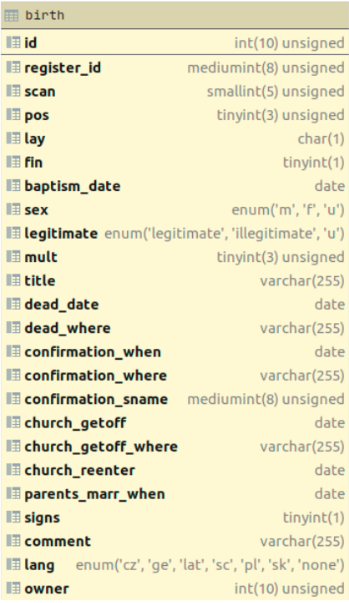
\includegraphics[width=0.5\textwidth]{obrazky-figures/birth_tabulka.png}
  \caption{Tabuľka so záznamom z matriky narodených}
  \end{center}
\end{figure}

Táto tabuľka predstavuje matričný záznam z matriky narodených. Vytvára sa nový objekt \textit{record}, do ktorého sa uložia informácie o zázname. Následne sa načítajú údaje
o prislúchajúcej matrike a uložia sa do objektu \textit{register}, ktorý reprezentuje matriku a
informácie o nej.\\
Ďalším krokom je získanie všetkých osôb. Tie sú uložené v tabuľke \textit{birthPerson}, ktorú môžete vidieť na obrázku \ref{birth}. Cez jednotlivé získané dáta o osobách sa ďalej
prechádza a získajú sa všetky potrebné informácie pre vytvorenie objektov \textit{Person}, ktoré
reprezentujú osoby figurujúce v zázname.

\subsubsection{Načítanie dát z grafovej databázy}
Z grafovej databázy sa načítavajú dáta pomocou dotazov v jazyku Cypher. Z grafovej
databázy potrebujeme získať údaje o osobách kvôli porovnaniu, preto sú dotazy cielené na
osoby a nie na záznamy. Dotazy v jazyku Cypher vrátia objekt typu slovník, ktorý má štruktúru uzla z Neo4j. V tomto objekte sú uložené všetky údaje o osobe,
s výnimkou adresy, ktorá je daná vzťahom \textit{BÝVA} medzi uzlami osôb a uzlami adries.\\
GPS súradnice sú načítané z JSON súborov a sú priradené obci ihneď potom čo sa obec
priradí osobe.

\subsubsection{Porovnávanie a klasifikácia}
Porovnanie osôb je rozdelené podľa ich pohlavia, pričom osoby s nedefinovaným pohlavím
sú porovnávané aj s mužmi aj so ženami. Prvým krokom porovnania je kontrola či osoba
v čase vzniku záznamu mohla žiť. V prípade splnenia tejto kontroly sa prechádza ku časti
základného porovnania, pri ktorom sa skontroluje meno, priezvisko, povolanie a mesto
v ktorom osoba žila. Ak sa ani jeden z týchto údajov medzi porovnávanými osobami
nezhoduje je dvojica označená ako nezhoda. V opačnom prípade sa pokračuje detailným
porovnaním ľudí. To je realizované v triede \textit{comparator}. Tu sú údaje porovnávané už
spomínanými metódami a z najlepších výsledkov jednotlivých porovnaní sa vytvára slovník \textit{comparison}. Porovnávanie často nekončí iba pri porovnaní osôb pôvodnej dvojice. Ak je to
možné porovnáva sa ďalej na základe vzťahov \textit{JE\textunderscore OTEC} a \textit{JE\textunderscore MATKA} a porovnanie
pokračuje rodičmi osoby z pôvodného porovnania. Rodič zo záznamu je vyhľadaný
v grafovej databáze a porovnanie pokračuje. Opäť vzniká objekt \textit{comparison} reprezentujúci
porovnávací vektor. Takýmto spôsobom sa pokračuje tak ďaleko ako nám povolí
spracovávaný matričný záznam. Všetky výsledky porovnaní sa ukladajú do zoznamu pre
výpočet     výsledného porovnania.\\\\
Po ukončení porovnávania sa spočítajú všetky hodnoty v slovníku \textit{comparison} vynásobené
ich príslušnými váhami, pričom hodnoty -1 označujú chýbajúci údaj a sú preto vynechané
z výpočtu. Výsledok je potom porovnaný s nastavenými prahmi a podľa toho klasifikovaný.
Návrh výsledného systému môžeme vidieť na obrázku \ref{navrh}.

\begin{figure}[h!]
  \label{navrh}
  \begin{center}
  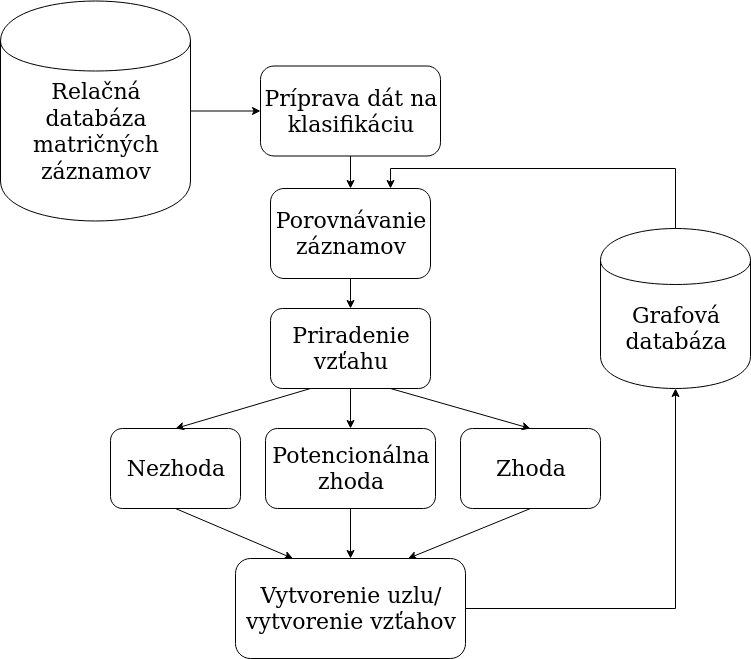
\includegraphics[width=0.7\textwidth]{obrazky-figures/navrh_riesenia2.png}
  \caption{Navrh prepojovania záznamov}
  \end{center}
\end{figure}
\newpage
\subsubsection{Uloženie záznamu}
Prvým krokom pri ukladaní záznamov je vytvorenie samotného uzlu so záznamom o krste.
Následne dôjde ku kontrole či matrika v ktorej bol záznam uložený už existuje ako uzol
v grafovej databáze. Ak nie, je vytvorený nový uzol s matrikou a ten je následne prepojený so
záznamom o krste použitím vzťahu \textit{JE\textunderscore V}. V prípade že matrika už existuje, dôjde iba ku
vytvoreniu prepojenia. Ďalej sa pokračuje podľa výsledku porovnania dvoch osôb.
V prípade že bola dvojica klasifikovaná ako nezhoda dôjde ku vytvoreniu nového uzla
s osobou. V prípade, že bola určená potencionálna zhoda dôjde taktiež ku vytvoreniu nového
uzla s osobou, ale v tomto prípade je nový uzol prepojený vzťahom \textit{POTENCIONALNI\textunderscore ZHODA} ku uzlu ku ktorému sa táto zhoda vzťahuje. V oboch prípadoch je
nutné vykonať kontrolu, či existuje uzol s adresou na ktorej daná osoba bývala. V prípade, že
adresa neexistuje je pridaná nová adresa. Údaj o adrese je zložený z uzlu obce či mesta,
ulice a popisného čísla, pričom medzi týmito uzlami funguje hierarchické prepojenie
pomocou vzťahu \textit{JE\textunderscore V}. Osoba je potom prepojená vzťahom \textit{BÝVA} na najdetailnejší údaj.
V prípade že adresa už existuje je iba vytvorené prepojenie medzi osobou a najdetailnejším
údajom z adresy. Pri vzťahu medzi adresou a osobou sa ukladá aj informácia o tom kedy
daná osoba na adrese bývala. V prípade klasifikácie dvojice osôb ako zhody dôjde ku
volaniu funkcie \textit{update\textunderscore node\textunderscore person} z triedy \textit{person.py}. Tá aktualizuje existujúci uzol o nové
hodnoty a dodatočné údaje ako napríklad povolanie, ktorých človek môže mať za život viac
uloží do listu. Po aktualizácii osoby v dôsledku zhody dôjde ku prehodnoteniu vzťahov
potencionálnych zhôd, ktoré sa môžu po doplnení nových údajov zmeniť. Ak dôjde ku
reklasifikovaniu potencionálnych zhôd na zhody proces sa opakuje. Potom čo sú vytvorené
všetky uzly začne prepájanie uzlov.\\\\
Metódou \textit{create\textunderscore connection\textunderscore with\textunderscore person\textunderscore in\textunderscore birth\textunderscore record} sa iteruje cez osoby a na základe
ich roly sú prepojené so záznamom a aj medzi sebou. Po vytvorení vzťahov medzi osobami
záznamu sa prechádza na ďalší záznam a proces sa opakuje kým nie je spracovaná celá
databáza. V tabuľke \ref{triedy} prevzanej zo zdroja \cite{formalniDP} môžeme vidieť prehľad všetkých modulov tvoriacich obsah práce.
\newpage

\begin {table}[ht]
\label{triedy}
\begin{center}
\begin{tabular}{ |c|c|} 

\hline
Triedy                           & Význam triedy \\ \hline

 main.py                         & Základný súbor, spracováva pripojenia  \\
                                 & na~databázu a~riadi testovanie \\\hline
 create\_database.py             & Hlavný algoritmus celého programu     \\   
                                 & riadi načítavanie záznamov, vytváranie grafovej\\
                                 & databázy a~spracováva výsledky porovnávania \\ \hline
 relational\_database\_birth.py  & Načítava dáta z~relačnej databázy \\ \hline
 graph\_database.py              & Načítava, aktualizuje, vyhľadáva, vytvára uzly  \\
                                 & a~prepojenia v~grafovej databáze  \\ \hline
 csv\_source.py                  & Načítava dáta z~CSV súborov  \\ \hline
 comparator.py                   & Porovnáva osoby a~vyhodnocuje výsledky,\\
                                 & obsahuje všetky metódy potrebné k~porovnávaniu  \\ \hline
 record.py                       & Trieda spravujúca záznam, obsahuje vytváranie  \\ 
                                 & uzlu, aktualizovanie uzlu, výpis informácii \\ \hline
 person.py                       & Trieda spravujúca osobu, vytváranie uzlu, \\
                                 & aktualizovanie uzlu, výpis informácií  \\ \hline
 register.py                     & Trieda spravujúca matriky, vytváranie uzlu,  \\
                                 & aktualizovanie uzlu, výpis informácií  \\ \hline
 domicile.py                     & Trieda spravujúca adresy, prehľadávanie json  \\
                                 & súborov, výpis informácií\\ \hline
 date.py                         & Trieda spravujúca dátumy \\ \hline
 get\_persons.py                 & Skript na~základe mena a~priezviská nájde všetky   \\                             
                                 & zodpovedajúce osoby uložené v~grafovej databáze\\  \hline
 get\_all\_records.py            & Skript na~základe id osoby nájde všetky záznamy \\
                                 & v~grafovej databáze, v~ktorých sa osoba nachádza \\ \hline
 get\_family\_tree.py            & Skript na~základe id osoby vypíše všetkých predkov  \\ 
                                 & a~potomkov ktorý sa nachádzajú v~grafovej databáze\\ 
\hline
\end{tabular}
\caption {Prehľad tried a~ich význam} \label{triedy}
\end{center}
\end {table}

\subsection{Dodatočné skripty}

Okrem programu realizujúceho hlavný algoritmus načítania, porovnávania, klasifikovania
a ukladania záznamov do grafovej databázy obsahuje práca Ing. Tušimovej aj ďalšie skripty
realizujúce operácie, ktoré sú z hľadiska genealogického výskumu zaujímavé. Skripty
realizujú dotazovanie nad grafovou databázou a vrátia výsledky vyhľadávania podľa
zadaných vstupných parametrov.

\subsubsection{get\textunderscore person.py}
Skript vráti výsledok vyhľadávania podľa mena a priezviska hľadanej osoby. Zobrazí všetky
informácie dostupné o tomto človeku. Prehľadávanie prebieha jednak s pôvodným menom
a aj s normalizovanou formou. Výstupom skriptu sú potom všetky informácie dostupné o danom človeku, vrátane jeho ID v grafovej databáze. To môže byť následne použité pri spúšťaní zvyšných skriptov, ktoré ako vstupný parameter vyžadujú ID osoby.

\subsubsection{get\textunderscore all\textunderscore records.py}

Skript realizuje vyhľadávanie na základe ID osoby. Skript získa a vypíše všetky záznamy
v ktorých hľadaná osoba figuruje ako aj všetky informácie o danej osobe a jej rolách
v konkrétnych záznamoch.

\subsubsection{get\textunderscore family\textunderscore tree.py}
Skript realizuje vyhľadávanie na základe ID osoby. Skript hľadá všetky osoby v prepojení \textit{JE\textunderscore MATKA, JE\textunderscore OTEC} oboma smermi. Teda hľadá predkov aj potomkov
zadanej osoby. Skript oboma smermi funguje rekurzívne a jeho výstupom je forma
rodokmeňu.

\chapter{Návrh}
V tejto kapitole si prejdeme návrh rozšírení a modifikácií, ktoré neskôr budú realizované
v rámci implementácie. Prejdeme si možnosti vylepšení algoritmu a rozšírení možností
vstupných dát. Ďalej si priblížime chyby a nedostatky zdrojovej práce, ktoré bolo nutné vyriešiť. Na záver sa pozrieme aj na možnosti optimalizácie a zvýšenia časovej efektivity skriptu.

\section{Rozšírenia}
V tejto podkapitole si ukážeme akou formou bude pôvodná práca rozšírená. Rozšírenia budú zamerná hlavne na pridanie nových typov záznamov a testovaní nových alternatív ku metrike použitej pre porovnávanie reťazcov v práci.

\subsection{Porovnávanie slov}
V tejto podkapitole sa pozrieme na rôzne alternatívy metrík použitých pri porovnávaní slov, ktoré by
mohli viesť ku lepším výsledkom, prípadne aj ku lepšej časovej efektivite programu.
Informácie v tejto podkapitole sú prevzaté zo zdroja \cite{strings}.
\newpage
\subsubsection{Jarova podobnosť}
Ak pri porovnávaní narazíme na meno, ktoré v databáze nemá normalizovanú formu,
používa sa pre určenie podobnosti mien už spomínaná Levenshteinova editačná
vzdialenosť. Existuje však prístup, ktorý by mohol byť pre porovnávanie kratších reťazcov vhodnejší a tým je Jarova podobnosť. Táto metóda je primárne určená pre kratšie reťazce a špecificky
napríklad pre mená a priezviská. Jej časová náročnosť by taktiež mala byť lepšia ako použitá
Levenshteinova editačná vzdialenosť. Metóda je podobne ako Levenshteinova vzdialenosť
založená na editačnej vzdialenosti dvoch reťazcov. Avšak okrem jednoznakových operácií
ponúkaných Levenshteinovou vzdialenosťou – vloženie, mazanie a substitúcia, pridáva
Jarova metóda ďalšiu operáciu, ktorou je transpozícia susedných znakov. Tento fakt je
obzvlášť relevantný, kvôli charakteru dát s ktorými sa táto práca zaoberá. Chyba zamenenia
susedných znakov v písaných textoch je jednou z najčastejších chýb, ktorých sa ľudia
dopúšťajú. Jarovu podobnosť \textit{sim\textsubscript{j}} dvoch reťazcov \textit{s\textsubscript{1}} a \textit{s\textsubscript{2}} vieme určiť týmto spôsobom:

\begin{equation*}
    sim\textsubscript{j} = 
\begin{cases} 0  &  ak \quad m = 0, \\
              \frac{1}{3} \cdot (\frac{m}{\mid s_{1}\mid} + \frac{m}{s_{2}} + \frac{m - t}{m})  &  inak \end{cases}
\end{equation*}

Kde $|s_{i}|$ udáva dĺžku reťazca $s_{i}$, $m$ udáva počet zhodujúcich sa znakov medzi dvoma
reťazcami a \textit{t} udáva počet transpozícií. Dva znaky patriace reťazcom \textit{s\textsubscript{1}} a \textit{s\textsubscript{2}} v tomto poradí
môžeme prehlásiť za zhodné ak sú znaky rovnaké a zároveň pre ich vzájomnú vzdialenosť \textit{d} platí nasledujúci vzťah:

\begin{equation*}
    d \leq \Bigg \lfloor \frac{max(|s_{1}|, |s_{2}|)}{2} \Bigg \rfloor - 1
\end{equation*}

Počet transpozícií je určený ako počet zhodujúcich sa znakov, ktorých sekvenčné poradie je
v porovnávaných reťazcoch odlišné vydelený dvomi.

\subsubsection{Jaro-Winklerova podobnosť}

Jaro-Winklerova podobnosť z princípu vychádza z Jarovej podobnosti, ale kladnejšie hodnotí
reťazce, ktoré sa zhodujú v prefixe až do dĺžky štyroch znakov. Pre určenie Jaro-Winklerovej
podobnosti \textit{sim\textsubscript{w}} dvoch reťazcov použijeme nasledujúci vzťah:

\begin{equation*}
    sim_{w} = sim_{j} + L \cdot p \cdot (1 - sim_{j})
\end{equation*}

Kde \textit{sim\textsubscript{j}} je hodnota Jarovej podobnosti dvoch reťazcov, \textit{L} udáva dĺžku spoločného prefixu
reťazcov až do maximálnej dĺžky prefixu 4 a \textit{p} je konštantná hodnota váhového faktoru so
štandardnou hodnotou \textit{p} = 0.1. Výraz (1 - \textit{sim\textsubscript{j}} nám udáva hodnotu Jarovej vzdialenosti (V
podstate ide o obrátenú hodnotu Jarovej podobnosti).
Táto metóda je obzvlášť relevantná, pretože ponúka výhody Jarovej podobnosti a k tomu
pozitívnejšie hodnotí reťazce so zhodným prefixom, čo je práve časté pri variáciách mien,
ktoré nemajú uloženú normalizovanú formu.

\subsubsection{Návrh implementovania metód}

Spomínané metódy je možné do programu implementovať viacerými spôsobmi. Keď
zohľadníme fakt, že metódy Jarovej vzdialenosti sú určené primárne pre kratšie reťazce a sú
obzvlášť efektívne pre porovnávanie mien, môžeme logicky dôjsť ku záveru, že bude vhodné
testovať dĺžku porovnávaných reťazcov pre určenie metódy, ktorá sa má použiť pre ich
porovnanie. Taktiež bude zohľadnený aj fakt, či ide o meno alebo priezvisko, ktoré pri
nenormalizovanej forme môžu zdieľať rovnaký prefix. Najlepší prístup bude určený
testovaním nad testovacími dátami a sledovaním presnosti klasifikácie záznamov a časovej
náročnosti výsledného algoritmu.

\begin {table}[ht]
\begin{center}
\begin{tabular}{ |c|c|} 
\hline
Premenná               & Typy porovnávania \\
\hline
 Meno                  & Presná zhoda, Levenshteinova vzdialenosť      \\
 Priezvisko            & Presná zhoda, Levenshteinova vzdialenosť      \\
 Povolanie             & Presná zhoda, Levenshteinova vzdialenosť      \\
 Mesto                  & Presná zhoda, vzdialenosť miest    \\
 Ulica                 & Levenshteinova vzdialenosť\\
 Popisné číslo         & Levenshteinova vzdialenosť, porovnávanie čísel  \\
 Dátum narodenia       & Levenshteinova vzdialenosť, kontrola dátumov,\\
                                     &  porovnanie veku\\
 Dátum (zvyšné typy)   & Levenshteinova vzdialenosť, kontrola dátumov \\
 Titul                 & Levenshteinova vzdialenosť \\
 Viera                 & Levenshteinova vzdialenosť \\
 Značky                & Presná zhoda   \\
\hline
\end{tabular}
\caption {Prehľad atribútov a spôsobov ich porovnávania} \label{porovavanie}
\end{center}
\end {table}

V tabuľke \ref{porovavanie} môžeme vidieť všetky atribúty a spôsob akým sú momentálne porovnávané. Po
zmenách v porovnávaní sa tabuľka zmení nasledujúcim spôsobom:

\begin {table}[ht]
\begin{center}
\begin{tabular}{ |c|c|} 
\hline
Premenná               & Typy porovnávania \\
\hline
 Meno                  & Presná zhoda, Jarova vzdialenosť      \\
 Priezvisko            & Presná zhoda, Jarova vzdialenosť      \\
 Povolanie             & Presná zhoda, Jarova vzdialenosť      \\
 Mesto                  & Presná zhoda, vzdialenosť miest    \\
 Ulica                 & Jarova vzdialenosť\\
 Popisné číslo         & Jarova vzdialenosť, porovnávanie čísel  \\
 Dátum narodenia       & Jarova vzdialenosť, kontrola dátumov,\\
                                     &  porovnanie veku\\
 Dátum (zvyšné typy)   & Jarova vzdialenosť, kontrola dátumov \\
 Titul                 & Jarova vzdialenosť \\
 Viera                 & Jarova vzdialenosť \\
 Značky                & Presná zhoda   \\
\hline
\end{tabular}
\caption {Prehľad atribútov a nových spôsobov ich porovnávania} \label{porovavanie_nove}
\end{center}
\end {table}

Je nutné si však uvedomiť, že pri porovnávaní niektorých atribútov bude stále možno použitá
Levenshteinova vzdialenosť, keďže tá môže byť efektívnejšia napríklad pri dlhších
reťazcoch. Bude preto nutné určiť istú formu hranice, pri ktorej sú výsledky dosiahnuté
použitím Jarovej vzdialenosti efektívnejšie, ako tie dosiahnuté použitím Levenshteinovej
vzdialenosti. Taktiež bude otestovaná efektivita Jaro-Winklerovej podobnosti a bude určený
najlepší prístup. Táto hranica bude teda určená testovaním. V tabuľke \ref{porovavanie_nove} môžeme vidieť
nové prístupy ku porovnávaniu jednotlivých atribútov.

\subsection{Ďalšie vstupné dáta}

V tejto podkapitole, si priblížime nové formy vstupných dát a urobíme základný návrh
pridania podpory.

\subsubsection{Matriky úmrtí a sobášov}

Práca Ing. Tušimovej momentálne pracuje iba s databázou obsahujúcou záznamy z matrík
narodených. Jednou z hlavných úloh mojej práce bude teda pridanie podpory pre záznamy
matrík sobášov a úmrtí. Toto bude realizované rovnakým spôsobom ako práca so
záznamami z matrík pôrodov. Pri hlavnom dotaze z funkcie v module \textit{create\textunderscore database.py}, ktorým
získavame všetky záznamy z matrík pôrodov si naberieme aj záznamy z matrík úmrtí
a sobášov. To znamená, že budeme musieť vytvoriť nové funkcie realizujúce dotazy na SQL databázu v module \textit{relational\textunderscore database\textunderscore birth.py} aby sme získali všetky ďalšie záznamy a v nich figurujúce osoby, pričom jednotlivým záznamom priradíme už predpripravený typ, podľa toho o aký
záznam pôjde. V práci bude použitá nová databáza typu MySQL s názvom demos. V tejto databáze už budú obsiahnuté aj záznamy o úmrtiach a sobášoch. Dotazy budú teda konkrétne na tabuľku \textit{burial}, v ktorej sú uložené záznamy z matrík úmrtí a tabuľku \textit{marriage}, v ktorej sú zasa záznamy o sobášoch.

\begin{longtable}{|l|c|c|c|}
 \caption{Štruktúra tabuľky burial} \label{tab:burial-structure} \\
 \hline \multicolumn{1}{|c|}{\textbf{Column}} & \multicolumn{1}{|c|}{\textbf{Type}} & \multicolumn{1}{|c|}{\textbf{Null}}\\ \hline \hline
\endfirsthead
 \caption{Štruktúra tabuľky burial (pokračovanie)} \\
 \hline \multicolumn{1}{|c|}{\textbf{Column}} & \multicolumn{1}{|c|}{\textbf{Type}} & \multicolumn{1}{|c|}{\textbf{Null}} \\ \hline \hline \endhead \endfoot
\textbf{\textit{id}} & int & No \\ \hline
register\_id & mediumint & No \\ \hline
scan & smallint & No \\ \hline
pos & tinyint & No \\ hline
lay & char(3) & Yes \\ \hline
fin & tinyint(1) & Yes \\ \hline
check\_req & tinyint(1) & Yes \\ \hline
lang & enum('CZ', 'GE', 'LAT', 'SC', 'PL', 'SK', 'NONE') & Yes \\ \hline
sex & enum('M', 'F', 'U', '[M]', '[F]') & Yes \\ \hline
dead\_born & tinyint(1) & Yes \\ \hline
viaticum\_date & char(10) & Yes \\ \hline
dead\_date & char(10) & Yes \\ \hline
burial\_date & char(10) & Yes \\ \hline
dead\_time & text & Yes \\ \hline
viaticum & tinyint(1) & Yes \\ \hline
burial\_place & text & Yes \\ \hline
death\_place & text & Yes \\ \hline
years & decimal(5,2) & Yes \\ \hline
months & decimal(5,2) & Yes \\ \hline
weeks & decimal(5,2) & Yes \\ \hline
days & decimal(5,2) & Yes \\ \hline
hours & decimal(5,2) & Yes \\ \hline
minutes & decimal(5,2) & Yes \\ \hline
death\_cause & mediumint & Yes \\ \hline
examination & tinyint(1) & Yes \\ \hline
marriage\_date & char(10) & Yes \\ \hline
marriage\_place & text & Yes \\ \hline
death\_address & int & Yes \\ \hline
birth\_address & int & Yes \\ \hline
baptised & tinyint(1) & Yes \\ \hline
legitimate & enum('legitimate', 'illegitimate', 'U') & Yes \\ \hline
marriage\_years & decimal(5,2) & Yes \\ \hline
comment & text & Yes \\ \hline
owner & int & Yes \\ \hline
score & double & Yes \\ \hline
last\_edited\_level & int & Yes \\ \hline
last\_edited\_highest\_level & int & Yes \\ \hline
 \end{longtable}

Z tabuľky \ref{tab:burial-structure} vidíme, že tabuľka záznamu o úmrtí obsahuje všetky potrebné informácie o zázname, ako jazyk v ktorom bol záznam napísaný, číslo skenu a pozícia na skene. Okrem toho záznam obsahuje aj id matriky, ktoré nám určuje matriku, z ktorej záznam pochádza. Ďalej sú tu aj relevantné informácie o zosnulom ako príčina smrti, dátum posledného zaopatrenia, úmrtia a pohrebu, pohlavie zosnulého, a fakt či nešlo o mŕtvorodené dieťa. Ďalej tabuľka samozrejme obsahuje unikátne ID, pomocou ktorého sa identifikujú všetky osoby figurujúce v danom zázname. Počet osôb figurujúcich v zázname o úmrtí je zo všetkých typov záznamov zvyčajne najnižší.

\begin{longtable}{|l|c|c|c|}
 \caption{Štruktúra tabuľky marriage} \label{tab:marriage-structure} \\
 \hline \multicolumn{1}{|c|}{\textbf{Column}} & \multicolumn{1}{|c|}{\textbf{Type}} & \multicolumn{1}{|c|}{\textbf{Null}} \\ \hline \hline
\endfirsthead
 \caption{Štruktúra tabuľky marriage (pokračovanie)} \\
 \hline \multicolumn{1}{|c|}{\textbf{Column}} & \multicolumn{1}{|c|}{\textbf{Type}} & \multicolumn{1}{|c|}{\textbf{Null}} \\ \hline \hline \endhead \endfoot
\textbf{\textit{id}} & int & No \\ \hline
register\_id & mediumint & No \\ \hline
scan & smallint & No \\ \hline
pos & tinyint & No \\ \hline
lay & char(3) & Yes \\ \hline
fin & tinyint(1) & Yes \\ \hline
check\_req & tinyint(1) & Yes \\ \hline
lang & enum('CZ', 'GE', 'LAT', 'SC', 'PL', 'SK', 'NONE') & Yes \\ \hline
banns1 & char(10) & Yes \\ \hline
banns2 & char(10) & Yes \\ \hline
banns3 & char(10) & Yes \\ \hline
marriage\_date & char(10) & Yes \\ \hline
kinship\_degree & varchar(50) & Yes \\ \hline
groom\_age\_year & decimal(5,2) & Yes \\ \hline
groom\_age\_month & decimal(5,2) & Yes \\ \hline
groom\_age\_day & decimal(5,2) & Yes \\ \hline
bride\_age\_year & decimal(5,2) & Yes \\ \hline
bride\_age\_month & decimal(5,2) & Yes \\ \hline
bride\_age\_day & decimal(5,2) & Yes \\ \hline
groom\_full\_age & char(10) & Yes \\ \hline
bride\_full\_age & char(10) & Yes \\ \hline
divorce\_date & char(10) & Yes \\ \hline
domicile & mediumint & Yes \\ \hline
unres\_descr\_num\_1 & char(10) & Yes \\ \hline
unres\_descr\_num\_2 & char(10) & Yes \\ \hline
groom\_birth\_address & int & Yes \\ \hline
groom\_dead\_address & int & Yes \\ \hline
bride\_birth\_address & int & Yes \\ \hline
bride\_dead\_address & int & Yes \\ \hline
signs & tinyint(1) & Yes \\ \hline
comment & text & Yes \\ \hline
owner & int & Yes \\ \hline
score & double & Yes \\ \hline
last\_edited\_level & int & Yes \\ \hline
last\_edited\_highest\_level & int & Yes \\ \hline
 \end{longtable}

Štruktúru tabuľky reprezentujúcej záznam o sobáši môžeme vidieť v tabuľke \ref{tab:marriage-structure}. Okrem rovnakých všeobecných informácií o samotnom zázname a matrike, ako aj v ostatných typoch záznamov, obsahuje informácie ako vek ženícha, vek nevesty, dátum sobášu, dátum rozvodu, a ďalej samozrejme aj unikátne id, pomocou ktorého dokážeme zistiť všetky osoby z tabuľky \textit{person} figurujúce v danom zázname. Naopak oproti záznamom úmrtia, obsahujú záznamy o sobášoch zvyčajne najviac figurujúcich osôb zo všetkých typov záznamov. Štruktúra tabuľky \textit{person} obsahujúcej informácie o jednotlivých osobách zo záznamu môžeme vidieť v tabuľke \ref{tab:person-structure}.

\begin{longtable}{|l|c|c|c|}
 \caption{Štruktúra tabuľky person} \label{tab:person-structure} \\
 \hline \multicolumn{1}{|c|}{\textbf{Column}} & \multicolumn{1}{|c|}{\textbf{Type}} & \multicolumn{1}{|c|}{\textbf{Null}} \\ \hline \hline
\endfirsthead
 \caption{Štruktúra tabuľky person (pokračovanie)} \\
 \hline \multicolumn{1}{|c|}{\textbf{Column}} & \multicolumn{1}{|c|}{\textbf{Type}} & \multicolumn{1}{|c|}{\textbf{Null}} \\ \hline \hline \endhead \endfoot
\textbf{\textit{id}} & int & No \\ \hline
birth\_id & int & Yes \\ \hline
marriage\_id & int & Yes \\ \hline
burial\_id & int & Yes \\ \hline
rel & enum & Yes \\ \hline
title & varchar(255) & Yes \\ \hline
sname & mediumint & Yes \\ \hline
domicile & mediumint & Yes \\ \hline
street & varchar(255) & Yes \\ \hline
descr\_num & char(10) & Yes \\ \hline
religion & enum('catholic', 'protestant', 'jew', 'none') & Yes \\ \hline
birth\_date & char(10) & Yes \\ \hline
dead & tinyint(1) & Yes \\ \hline
waif & tinyint(1) & Yes \\ \hline
category & char(1) & Yes \\ \hline
person\_relation & mediumint & Yes \\ \hline
widow & tinyint(1) & Yes \\ \hline
legitimate & enum('legitimate', 'illegitimate', 'U') & Yes \\ \hline
dead\_date & char(10) & Yes \\ \hline
work\_place & text & Yes \\ \hline
age & decimal(3,2) & Yes \\ \hline
 \end{longtable}

Každá osoba uložená v tejto tabuľke predstavuje jednu osobu figurujúcu v práve jednom zázname. Vzťah medzi osobu a záznamom je daný pomocou príslušného ID záznamu. Pôjde teda o jednu z hodnôt \textit{birth\textunderscore id}, \textit{marriage\textunderscore id} a \textit{burial\textunderscore id}. Ako hodnota v týchto stĺpcoch je použité ID záznamu, do ktorého daná osoba prináleží. Je tu preto pridaný cudzí kľúč vo forme daného ID, odkazujúceho na konkrétny záznam. Každá osoba uložená v databáze môže prináležať práve do jedného záznamu. Ďalej tabuľka obsahuje stĺpec \textit{rel}, ktorého hodnotou je jeden zo vzťahov. Tie sú reprezentované typom enum, kde sú všetky jednotlivé vzťahy vymenované. Potom tu máme informácie o dátume narodenia, smrti, veku a ďalších dodatočných informácií.
Ďalej uplatníme rovnaký postup porovnávania osôb zo záznamov ako doteraz, ale pri vytvorení nových prepojení medzi dvoma osobami a osobou a záznamom budeme musieť vytvoriť nové funkcie ktoré budú realizovať prepojenie osôb podľa ich úlohy v danom zázname. Pri práci s testovacou sadou pôjde o rovnaký postup.

\subsubsection{Rozšírenie funkcií}

V module \textit{relational\textunderscore database\textunderscore birth.py}, ktorý načítava záznamy z matrík, ale aj v ďalších častiach
programu bude potom nutné pridať kontroly zisťujúce o aký typ záznamu sa jedná. Ku každej funkcii určenej pre spracovanie záznamov o krste bude nutné vytvoriť ekvivalentnú funkciu určenú pre iný typ záznamu a prípadne na miestach, kde to bude možné, rozšíriť už existujúce funkcie tak, aby fungovali pre všetky typy záznamov. Vo výstupnej grafovej
databáze bude nutné zaviesť niekoľko nových typov uzlov. Pôjde u uzly \textit{Záznam\textunderscore o\textunderscore úmrtí} a \textit{Záznam\textunderscore o\textunderscore sobáši}. Taktiež dôjde ku pomerne veľkému rozšíreniu typu vzťahov, kde bude
nutné pridať vzťahy pre všetky nové spojenia podľa formátu nových dát. Všetky pridané vzťahy a všetky rozšírenia budú popísané ďalej v práci v časti implementácie.
\nocite{*}

\section{Analýza efektivity a problémov algoritmu}

Hlavným problémom algoritmu v pôvodnej podobe bola jeho vysoká časová náročnosť. Tá je spôsobená neustále sa zvyšujúcim počtom osôb ktoré musíme spracovať. Kvôli charakteru práce je nutné vykonávať stále viac a viac porovnaní, keďže sú osoby porovnávané spôsobom každá s každou. Pri každej porovnávanej osobe nám teda počet porovnaní vzrastie o 1. Preto môžeme hovoriť o polynomiálnej časovej komplexite a vyjadriť ju ako:

\begin{equation*}
    O(\frac{n^2 - n}{2})
\end{equation*}

kde \textit{n} je počet osôb, ktoré tvoria vstup algoritmu. Tento predpoklad môžeme učiniť, pretože počet porovnaní priamo úmerne odpovedá dobe trvania a aj keď niektoré porovnania vedú ku identifikácii zhodných osôb a ich následnému zjednoteniu, čo má síce efekt na dobu trvania programu, ide stále o zriedkavú udalosť v porovnaní s bežným scenárom pridania novej osoby, prípadne osoby identifikovanej ako potencionálne zhodnej osoby. Môžeme preto túto skutočnosť zanedbať. Taktiež môžeme pre účely určenia časovej komplexity zanedbať aj fakt, že sú na mieste viaceré optimalizačné metódy, ako napríklad porovnávanie osôb iba s osobami rovnakého pohlavia, alebo neporovnávanie osôb s osobami z rovnakého záznamu. Je nutné sa preto zamerať na zníženie doby trvania spracovávania jednej osoby.

\subsection{Zistenie doby trvania spracovávania}

Pre zistenie priemernej doby spracovania jednej osoby bol použitý nástroj cProfile \cite{cProfile}. Ten je ideálny pre zistenie času behu jednotlivých funkcií a identifikáciu najpomalších úsekov. Keďže potrebujeme zistiť priemernú dobu trvania jedného porovnania a spracovania osoby, môžeme sa pozrieť na celkový čas strávený vo funkcii riadiacej spracovanie jedného záznamu. To síce nie je presná doba spracovania jednej osoby, ale priamo úmerne jej zodpovedá a je to spôsob ako dostaneme najrelevantnejšiu hodnotu ktorá vypovedá o dobe trvania programu bez toho, aby sme zanedbali réžiu nad spracovávaním osôb, ktorá okrem porovnávania zahŕňa vytváranie a prepájanie osôb so záznamami a medzi sebou. Budeme teda skúmať dobu trvania funkcie \textit{compare\textunderscore record\textunderscore with\textunderscore graph\textunderscore database}. Tá dostane ako parameter záznam a spracuje všetky osoby, ktoré v ňom figurujú. Profiling bol vykonaný nad vzorkou o veľkosti tisíc záznamov krstu z databázy perun. Celkový čas, ktorý bol strávený spracovávaním záznamov, bol 17237 sekúnd, čo sú asi 4 hodiny a 47 minút. Celkovo bolo spracovaných 8271 osôb. Ak teda vydelíme túto dobu trvania počtom spracovaných osôb, dostaneme požadovanú priemernú dobu trvania spracovávania jednej osoby. Po tejto jednoduchej kalkulácii nám vychádza, že táto doba je 2,084 sekundy. Túto hodnotu si neskôr porovnáme s novou hodnotou získanou rovnakým spôsobom po všetkých zmenách vykonaných v tejto práci, aby sme videli o koľko je výsledný algoritmus efektívnejší. Jediné čo sme pri tomto výpočte z celkovej doby trvania programu zanedbali je doba pripojenia ku databázam, mazanie už existujúcich dát z Neo4j databázy a dotazovanie nad MySQL databázou. Doba trvania týchto častí bude rovnaká i po zmenách uskutočnených v tejto práci, a preto ju nebudeme brať do úvahy.

\subsection{Identifikovanie časovo náročných miest v programe}
Proces identifikovanie časovo najpomalších úsekov programu pozostával z vyhľadania funkcií na čo najnižšej úrovni, teda funkcií, ktoré ďalej obsahujú čo najmenší počet, či ideálne žiadne volania ďalších zanorených funkcií. Na to nám opäť slúžil cProfile. Pomocou neho som zistil, že drvivá väčšina času behu programu je strávená v module \textit{graph\textunderscore database.py}. Konkrétne išlo hlavne o funkciu \textit{run\textunderscore cql\textunderscore with\textunderscore return\textunderscore person}, ktorá využíva funkcie \textit{run} a \textit{data} z knižnice neo4j na vykonanie dotazov a navrátenia dát získaných v týchto dotazoch. Táto funkcia zodpovedá drvivej väčšine doby behu programu (vyše 16000 sekúnd). Počas celého procesu porovnávania je nutné pracovať s osobami, ktoré sú už uložené v grafovej databáze. Preto dochádza ku neustálemu dotazovaniu nad grafovou databázou na osoby a aj na ich adresy. Keďže pri skončení porovnávania jedného záznamu a teda aj osôb v ňom sa databáza zmenila (boli pridané nové osoby a prepojenia) je nutné toto dotazovanie opakovane vykonávať zakaždým, keď potrebujeme nejaké dáta. Z toho nám vyplýva, že vysoká doba trvania programu je spôsobená najmä spôsobom, akým sa pracuje s grafovou databázou. Problém teda vznikol už v samotnom návrhu pôvodnej práce.

\subsection{Nový návrh výsledného systému}
Keďže už vieme, kde sa skrýva najväčší nedostatok výsledného systému, môžeme sa pozrieť na spôsob, akým by sme ho mohli prerobiť tak, aby bol vo výsledku efektívnejší.

\begin{figure}[t]
\label{system}
\centering
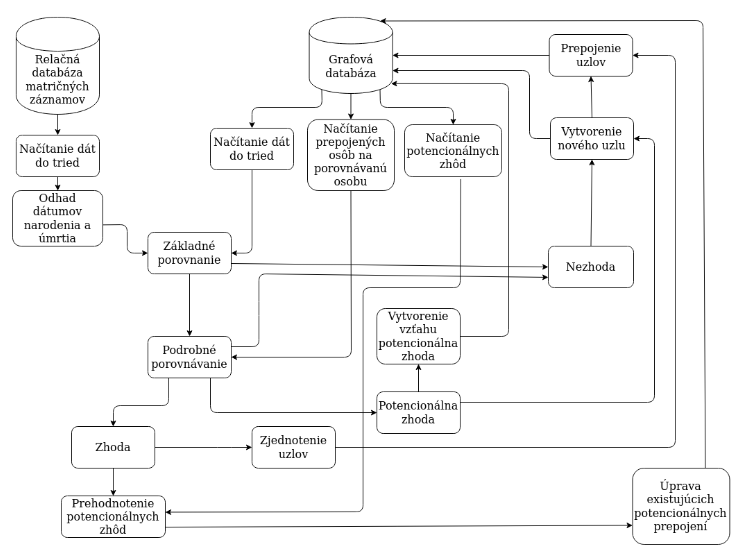
\includegraphics[width=1\textwidth]{obrazky-figures/diagram-original.PNG}
\caption{Návrh celého systému v pôvodnej forme}
\end{figure}

Na obrázku \ref{system} prevzatom zo zdroja \cite{formalniDP} môžeme vidieť celý návrh pôvodného systému. Keďže vieme, že problém je v práci s grafovou databázou, budú sa zmeny musieť týkať hlavne tejto časti. Pokúsime sa teda eliminovať časť neustáleho načítania dát z grafovej databázy, teda úseky \textit{Načítanie dát do tried}, \textit{Načítanie prepojených osôb na porovnávanú osobu} a \textit{Načítanie potencionálnych zhôd}. Jedným z riešení, ktoré som pri vytváraní výsledného návrhu skúmal bolo udržiavať časť dát z grafovej databázy v objektoch jazyku python a minimalizovať tak počet dotazov na databázu. Tým pádom by sme si dáta natiahli iba raz, a pri ukladaní nových osôb do grafovej databázy by sme si tieto osoby pridali aj do spomínaných objektov. Problémom tohoto spôsobu čiastočnej optimalizácie bol však fakt, že pri ukladaní osôb do databázy často dôjde ku zmene vzťahov a aj informácií o osobách, či prípadnému mazaniu a zjednocovaniu osôb. Okrem toho by sa nejednalo o najlepší spôsob optimalizácie z dôvodu, že stále musíme opakovane pristupovať do grafovej databázy, a to nie len pre ukladanie osôb, ale aj pri zjednocovaní uzlov osôb, prepájaní vzťahov, mazaní uzlov osôb alebo aj aktualizácii pri nájdení zhodnej osoby. Pre dosiahnutie najlepšej optimalizácie výsledného systému by sme teda potrebovali okrem neustáleho načítania dát eliminovať aj časť neustáleho vkladanie dát do grafovej databázy. Tu sa ukázalo ako najefektívnejšie riešenie nepracovať s grafovou databázou počas procesu porovnávania vôbec. Všetky dáta, ktoré boli pôvodne držané v grafovej databáze by sme teda potrebovali reprezentovať výhradne pomocou objektov jazyku python. Tu si musíme uvedomiť, že aby sme toto mohli vykonať, bude nutné už existujúce objekty reprezentujúce osoby, záznamy ale aj ďalšie uzly z neo4j podstatne rozšíriť takým spôsobom, aby sme mohli reprezentovať všetky spojenia, ktoré budú existovať vo výslednej databáze v reálnom čase. Bude preto nutné vytvoriť novú triedu pre spravovanie všetkých python objektov držaných výhradne v pamäti a pre vykonávanie operácii nad nimi.

\begin{figure}[h]
\label{after}
\centering
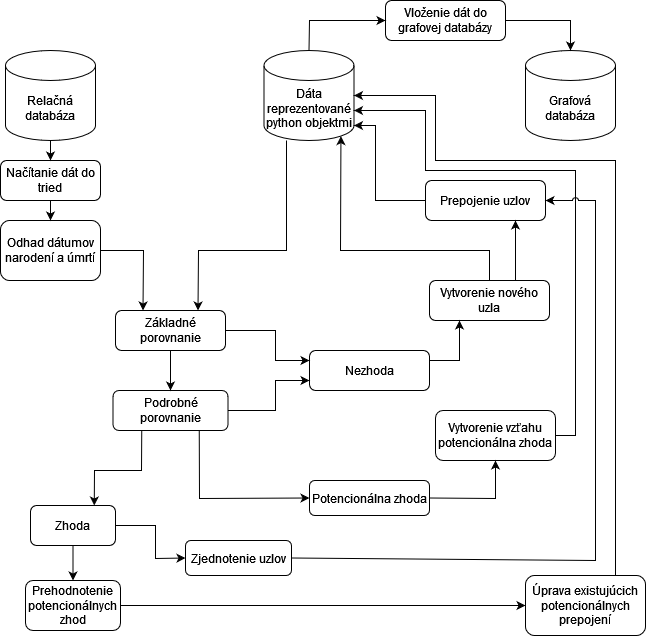
\includegraphics[width=1\textwidth]{obrazky-figures/Untitled Diagram.drawio.png}
\caption{Návrh výsledného systému}
\end{figure}

Z obrázku \ref{after} môžeme vidieť, že v takto zmenenom systéme sa budú dáta držať v pamäti na hromade a budú uložené v python objektoch, odpovedajúcich štruktúre a vzťahom z grafovej databázy. Tým by sme eliminovali proces neustáleho vytvárania a vykonávania dotazov v jazyku cypher nad v istom bode už pomerne objemnou databázou. Na konci porovnávania budú dáta do grafovej databázy vložené naraz až vo výslednej podobe. V takomto prístupe však existuje aj nevýhoda oproti pôvodnej implementácii a to je fakt, že na to, aby sme dostali finálny výstup v podobe grafovej databázy musíme počkať do konca procesu porovnávania a vkladania. Toto však nie je veľmi podstatné, keďže je skript možné jednoducho modifikovať takým spôsobom, aby spracoval iba fixný počet záznamov, napríklad pomocou jednoduchého počítadla v hlavnom cykle (napríklad pri testovacom spúštaní skriptu).

\chapter{Implementácia}

V tejto kapitole sa budeme venovať analýze a oprave chýb a prípadných nedostatkov práce, ďalej si povieme niečo ku implementácii nového prerobeného algoritmu, hlavne pri práci s grafovou databázou, kde dochádza ku výraznému spomaleniu algoritmu. Potom sa pozrieme na presný spôsob implementácie rozšírení týkajúcich sa nových matrík (teda nových typov záznamov o sobáši a úmrtí) vrátane zmien potrebných pri prechode na novú relačnú databázu demos, ktorej štruktúra sa mierne zmenila. Na záver si ukážeme novú formu výstupu vo vyhľadávacích skriptoch a ako boli implementované nové metriky použité pri porovnávaní.

\section{Identifikovanie nedostatkov}

Hľadanie nedostatkov a chýb a ich následné riešenie sa ukázalo byť jedným z najkomplikovanejších a časovo najnáročnejších aspektov tejto práce. Bolo tomu tak najmä kvôli veľkému rozsahu zdrojového kódu skriptov, ale aj kvôli vysokému počtu modulov, ktoré sú navzájom všetky prepojené. Ku odhaleniu chýb došlo najmä pri neustálom spúšťaní skriptu nad rozlyčnými dátami, či už z databázy alebo zo súborov csv, a postupným prechádzaním zdrojového kódu. Často sa ani nejednalo vyslovene o chyby, ale skôr nedostatky, ktoré sa ukázali ako zbytočné, či prípadne o funkcionality, ktoré bolo možné implementovať efektívnejším spôsobom. Väčšina chýb sa týkala práce s grafovou databázou Neo4j a dotazov nadňou, ale niekoľko problémov bolo i v reprezentácii dát a samotnom porovnávaní osôb. V tejto podkapitole si priblížime proces identifikovania chýb a konkrétne chyby a nedostatky, na ktoré som počas vypracovávania práce narazil. Pri každom probléme ukážem aj ako som ho vyriešil.

\subsection{Počiatočné úpravy}

V tejto sekcii si ukážeme ako bolo nutné skript upraviť, aby bol opäť funkčný.

\subsubsection{Identifikovanie problému}

Pred začatím akéhokoľvek implementovania navrhnutých zmien bolo nutné skript najprv upraviť, kedže v stave v akom som ho dostal ho nebolo možné spustiť. Išlo o chybu v module \textit{graph\textunderscore database.py}, pri ktorej sa vo funkcii, ktorá vytvárala dotaz v jazyku cypher, ktorý mal získať všetky adresy osoby z grafovej databázy pristupovalo ku python štruktúre typu slovník na neexistujúci kľúč. Tento slovník mal reprezentovať osobu z grafovej databázy, avšak žiaden kľúč pre ID osoby v slovníku nebol. Dôvodom pre toto mohlo byť, že niektoré zo starších verzií grafovej databázy Neo4j alebo ovládača pre túto databázu v štruktúre typu slovník reprezentujúcej uzol získaný z databázy uvádzali aj ID uzla. Rovnaký problém mali aj niektoré ďalšie funkcie v module s grafovou databázou.

\subsubsection{Riešenie problému}

Keďže ID osoby nebolo v spomínanej funkcii s názvom \textit{get\textunderscore addresses\textunderscore of\textunderscore person\textunderscore from\textunderscore graph\textunderscore db} dostupné, nebolo možné túto querry vytvoriť a spustiť nad databázou. Bolo preto nutné ID osoby nejakým spôsobom získať a propagovať do tejto funkcie. Jednoduchým riešením, ktoré mi napadlo bolo pridať ID samotného uzla ako atribút osoby, tým pádom by sme pri každej osobe získali aj ich ID. Preto som pri vytváraní osôb z grafovej databázy pridal atribút, ktorý sa pri vytvorení uzla nastaví na ID samotného vytváraného uzla.

\subsection{Pohlavia osôb}
Pri určení cieľovej skupiny, s ktorou má daná osoba zo záznamu byť porovnávaná na základe pohlavia dochádzalo pri každej osobe k tomu, že sa porovnávala so všetkými osobami namiesto toho, ako bolo pôvodne zamýšľané (teda iba s osobami rovnakého pohlavia). Zdrojové dáta boli v poriadku a pohlavia osôb boli v databáze i csv súboroch uložené tak, ako mali byť, teda správne označené ako 'M' - muž (male), 'F' alebo 'Ž' - ako žena (alebo female) a pri neidentifikovanom pohlaví ako 'U' - unidentified. Problémom bol spôsob kontroly pohlaví pri spracovávaní osôb. Z dôvodu účelu práce musí každý atribút objektov reprezentujúcich uzly z databázy Neo4j byť uložený ako list. Je tomu tak preto, že niektoré vlastnosti môžu mať v databáze viacero hodnôt a aj kvôli tomu, že pri aktualizácii informácií osoby pri zjednocovaní uzlov osôb si je nutné ponechať všetky informácie, jednak o pôvodnej osobe a aj o osobe, ktorú s ňou zjednocujeme. Pri kontrole pohlavia sa tento fakt však nezohľadňoval a pohlavie sa nesprávne porovnávalo ako objekt typu list, namiesto konkrétnej hodnoty v tomto liste. Tým pádom sa skript vždy vydal do tej istej vetvy a to síce tej, kde pohlavie osoby bolo označené za neidentifikované.
\newline

Riešenie tohoto problému bolo triviálne, preto si ho zhrnieme iba veľmi stručne. Na mieste kontroly pohlaví je pridaná jednoduchá kontrola toho, koľko hodnôt má táto osoba v tomto atribúte. V prípade, že je hodnota jedna, tak pohlavie určíme jednoducho pomocou pristúpenia na túto hodnotu. V prípade že sú v liste dve hodnoty, skontrolujeme, či sú obidve hodnoty iba znaky 'Z' alebo 'F', označujúce ženské pohlavie. V opačnom prípade môžeme prehlásiť, že výsledné pohlavie osoby je nedefinované, kvôli rôznym hodnotám tohoto atribútu. To isté môžeme taktiež prehlásiť, ak sú pohlavia v liste viac ako dve.

\subsection{Porovnávanie osôb spolu s predkami}

Pri analýze kódu som narazil na chybu, ktorá spôsobovala, že predkovia osoby zo záznamu boli porovnávaní s nesprávnym predkom osoby z grafovej databázy. Rola osoby je identifikovaná pomocou reťazca, ktorý je rovnaký ako enumeračný typ určený pre roly osôb z databázy. Šlo o prípad, kedy boli porovnávaní rodičia osoby zo záznamu. Tých reprezentujú roly, ktoré majú v programe názov \textit{f} a \textit{m}. Chyba nastala ak sme chceli porovnávať rodičov rodičov, teda starých rodičov hlavnej osoby zo záznamu. Pri porovnaní predkov osoby je samozrejme žiadúce porovnávať osoby v rovnakom vzťahu ku pôvodnej osobe. Napríklad pri porovnávaní osoby, ktorá má v zázname rolu otcova matka (teda vzťah reprezentovaný ako reťazec \textit{f\textunderscore m}) je žiadúce túto osobu porovnávať s osobou z grafovej databázy, ktorá má ku pôvodnej osobe rovnaký vzťah. Avšak vo funkcii realizujúcej toto porovnanie s názvom \textit{comparison\_of\_two\_person\_with\_ancestors} tomu tak nebolo. Namiesto toho, aby sme osobu vo vzťahu otcova matka porovnávali aj s otcovou matkou zo záznamu, bola osoba z grafovej databázy porovnávaná s osobou s rolou \textit{m\textunderscore f}, teda matkin otec. Rovnako tomu bolo aj v opačnom prípade, teda v prípade porovnania matkinho otca, ktorý bol nesprávne porovnávaný s otcovou matkou. Toto mohlo mať mierny negatívny vplyv na výsledky porovnaní. Oprava chyby spočívala iba v zmenení hodnôt reprezentujúcich rolu osoby na správnu hodnotu.

\subsection{Práca s dátumami}

V tejto podsekcii si povieme, ako sa v pôvodnej implementácii pracovalo s dátumami a ukážeme si, ako sa s nimi bude pracovať po vykonaných zmenách.

\subsubsection{Modul date.py}

Pre prácu s dátumami sa v implementácii používa modul \textit{date.py}. V tomto module sa nachádza trieda \textit{Date}. Jej atribútmi je celý objekt dátumu v podobe objektu typu datetime, rok, mesiac a deň dátumu. Trieda ďalej ponúka viacero funkcií realizujúcich vyžadované operácie nad objektami vytvorenými z tejto triedy, ako napríklad úpravu dátumu pri dni, ktorý je mimo rozsah daného mesiaca, funkciu pre vytvorenie objektu \textit{Date} zo vstupného reťazca či metódu pre výpis dátumu. Pri analýze kódu som došiel ku záveru, že je tento modul zbytočný. Jediná funkcionalita, ktorú ponúka naviac v porovnaní s klasickým python modulom pre reprezentáciu a prácu s dátumami \textit{datetime}, je implementovaná funkcia \textit{change\textunderscore date\textunderscore to\textunderscore nearest\textunderscore possible}. Tá pri dni v mesiaci, ktorý je mimo rozsah daného mesiaca posunie dátum na najbližší ďalší existujúci deň. Avšak implementáciou podobnej funkcie v module \textit{relational\textunderscore database\textunderscore birth.py}, ktorú je nutné aj tak implementovať, kvôli chýbajúcim údajom v dátumoch v novej použitej databáze demos, ktoré bude nutné aj tak nahradiť existujúcou hodnotou. Ďalším dôvodom prečo bolo výhodné tento modul odstrániť bol fakt, že pri prerábaní systému došlo ku viacerým rozsiahlým zmenám a s modulom sa v porovnaní s modulom \textit{datetime} pracuje zbytočne o dosť viac komplikovane, keďže je nutné pre výpis, konverziu či načítanie a uloženie dát volať špeciálne funkcie tohto modulu, nehovoriac o fakte, že modul je v podstate iba komplikovanejší spôsob uchovávania objektu triedy \textit{datetime.datetime} s dodatočnými krokmi.

\subsubsection{Odstránenie modulu}

Modul som sa rozhodol z implementácie odstrániť úplne a namiesto objektov, ktoré implementuje trieda \textit{Date} som sa rozhodol pre reprezentovanie a prácu s dátumami použiť existujúci modul \textit{datetime}, ktorý ponúka triedu \textit{datetime.datetime}. Ten je pre reprezentáciu dátumov ideálny a ponúka všetky potrebné funkcionality implementované pôvodným modulom, ako funkcie \textit{strptime} a \textit{strftime}, ktoré umožnujú jednoducho konvertovať reťazce na \textit{datetime.datetime} objekty a naopak.

\subsubsection{Nutné zmeny po odstránení}

Po odstránení modulu bolo nutné vykonať viacero zmien. Išlo o zmeny pri určovaní dátumov podľa rôl osôb, načítaní dát a v podstate na každom mieste v kóde, kde dochádzalo ku porovnaniam medzi dátumami a prevodom z reťazca na typ reprezentujúci dátum a naopak. V module \textit{relational\textunderscore database\textunderscore birth.py} bolo nutné potom implementovať požadovanú funkcionalitu zmenenia neexistujúcich dátumov na existujúce a to pomocou funkcie \textit{replace\textunderscore double\textunderscore questionmarks}, ktorá vykonáva doplnenie chýbajúcich dát takým spôsobom, že v prípade chýbajúceho dňa a mesiaca je deň alebo mesiac nastavený na prvý deň v mesiaci alebo teda prvý mesiac v roku. Funkcia zohľadňuje aj počet dní, ak vieme o aký mesiac sa jedná a naopak, ak by bol deň mimo rozsah mesiaca, vyberie iba odpovedajúce mesiace, ktoré môžu daný počet dní mať. Okrem funkcie sú na mieste spracovania dátumov aj ďalšie kontroly, či napríklad nedošlo ku zameneniu údaju o dni s údajom o mesiaci. Toto môžeme prehlásiť, ak je údaj dňa menší ako 12 a údaj o mesiaci väčší ako 12. V takomto prípade sa predpokladá zamenenie hodnôt a hodnoty údajov sú vymenené.

\subsection{Mazanie databázy}

V tejto sekcii si priblížime problém, ktorý vznikol pri mazaní databázy, ktorá bola naplnená vysokým objemom dát.

\subsubsection{Identifikovanie problému s mazaním}

Počas testovania nad databázou som narazil na problém, ku ktorému dochádzalo pri snahe zmazať celú databázu pri novom spustení skriptu. Keďže Neo4j community edition neponúka možnosť databázu zmazať pomocou drop dotazu (funkcionalita je dostupná iba pre Neo4j enterprise edition), bola databáza mazaná vytvorením dotazu odpovedajúcemu všetkým prvkom databázy a následnému zmazaniu všetkých vzťahov a uzlov.

\begin{figure}[h]
\label{deletion}
\begin{lstlisting}[language=SPARQL]
                            MATCH (n) DETACH DELETE n
\end{lstlisting}
\caption{Dotaz používaný na mazanie databázy}
\end{figure}

Na obrázku \ref{deletion} môžeme vidieť dotaz realizujúci mazanie v pôvodnej implementácii. Problém nastáva vtedy, keď je v databáze veľký objem dát a z tohto dôvodu pri snahe o vytvorenie takéhoto dotazu dôjde ku chybe typu java heap error. To znamená, že pri snahe pomocou dotazu označiť príliš veľké množstvo dát dôjde jazyku java, v ktorom je databáza Neo4j implementovaná pamäť na hromade.

\subsubsection{Možné riešenia}

Na vyriešenie tohoto problému sa ponúkalo viacero spôsobov. Prvým by bolo zo skriptu za použitia python modulu s názvom \textit{os} manuálne pristúpiť a zmazať zdrojové súbory databázy. Avšak problémom tohto riešenia je, že skript by potom musel byť vždy spúšťaný s administrátorskými právami, čo nie je veľmi praktické. Taktiež by vznikol problém pri zisťovaní cesty k týmto súborom, keďže databáza Neo4j môže byť nainštalovaná na rôznych miestach a súbory s databázou môžu mať podľa platformy, na ktorej je databáza nainštalovaná rôzne umiestnenie. Toto riešenie preto nie je veľmi vhodné. Ďalšou možnosťou by bolo manuálne zvýšenie množstva pamäťe na hromade, ktoré java priraďuje aplikácii Neo4j. Avšak tu sa nejedná o úplné riešenie problému, ale skôr iba o odsunutie. Potom by tu bola možnosť prechodu z Neo4j Community Edition na Neo4j Enterprise Edition. Táto edícia databázy je však platená a kvôli jedinej požadovanej funkcionalite by to bolo zbytočné. Najlepším riešením sa ukázalo byť mazanie databázy v menších dávkach (tzv. batch deletion). To ale nie je možné vykonať pomocou jediného dotazu. Bolo preto nutné pridať jednoduchý algoritmus realizujúci opakované cypher dotazy dovtedy kým databáza nie je prázdna.

\begin{figure}[h]
\label{batchdelete}
\centering
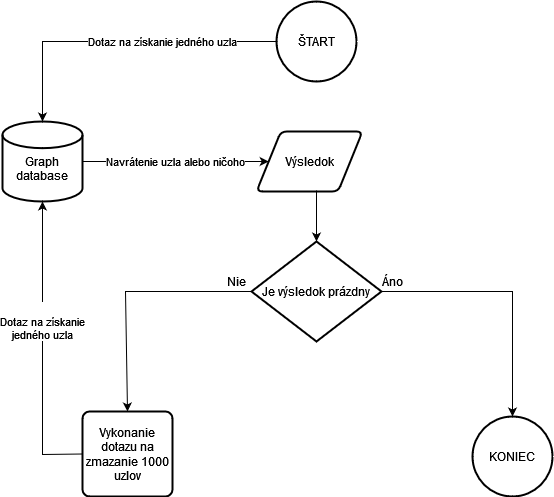
\includegraphics[width=0.8\textwidth]{obrazky-figures/Database-deletion.png}
\caption{Schéma algoritmu mazania}
\end{figure}

Na obrázku \ref{batchdelete} môžeme vidieť algoritmus mazania databázy. Na začiatku sa vykoná jednoduchý dotaz na získanie jediného uzla. Vo výsledku dotazu následne skontrolujem, či nie je prázdny. V prípade, že je výsledok prázdny môžeme prehlásiť databázu za prázdnu a teda pokračovať vo vykonávaní samotného skriptu. V prípade, že výsledok dotazu nie je prázdny, vykonáme dotaz na zmazanie tisícich uzlov z databázy. Ďalej pokračujeme rovnakým dotazom na získanie jediného uzla z databázy a proces sa takto opakuje, až kým databáza nie je prázdna.

\subsection{Ďalšie optimalizácie}

V skripte bolo vykonaných množstvo ďalších menších optimalizácií, ktoré samé o sebe veľmi nestoja za zmienku. Išlo najmä o odstránenie zbytočných funkcií realizujúcich triviálne operácie. Jedná sa o funkcie, ktoré mohli byť napríklad nahradené jednou podmienkou, alebo realizujúcich minimálne množstvo kódu, teda iba pridávali extra réžiu spôsobenú svojím volaním. Ďalšou optimalizáciou, ktorá možno stojí za zmienku je nahradenie neustálého používania operátora \textit{+} jazyka python pre konkatenáciu reťazcov. Ten môže byť pri konkatenácii väčšieho množstva reťazcov výrazne menej efektívny ako metóda \textit{join} z modulu \textit{string}. Tá môže byť podľa informácií zo zdroja \cite{plusop} až 4-krát efektívnejšia pri konkatenácii viacerých reťazcov ako operátor \textit{+}. Takéto optimalizácie nemusia mať pri spracovávaní menšieho množstva dát veľmi výrazný efekt, ale pri spracovávaní veľkého objemu dát sa už môže jednať o signifikantné množstvo ušetreného času, hlavne ak si uvedomíme, že počas behu skriptu dochádza ku konkatenácii reťazcov pomerne často.

\subsection{Skript get\_all\_records.py}

Tento skript bol v pôvodnom stave implementácie nefunkčný. Pri získavaní dát o úlohe osoby v špecifickom zázname a pri získavaní dátumu záznamu sa ku navrátenej štruktúre s týmito údajmi pristupovalo nesprávne. Tento problém bol jednoducho vyriešiteľný úpravou spôsobu, akým sa k týmto dátam pristupuje.

\section{Implementácia zmeneného systému}

V tejto podkapitole si povieme ako prebiehala a čo všetko zahŕňala implementácia nového navrhnutého systému. Postupne si prejdeme jednotlivé zmeny, ktoré táto optimalizačná zmena priniesla.

\subsection{Rozbor problematiky}

Hlavným riadiacim bodom celého algoritmu je modul \textit{create\_database.py}. Ten riadi celý proces porovnávania a spracovávania dát. Celý proces pozostáva z načítania dát z relačnej databázy pomocou metód z triedy \textit{RelationalDatabaseHandle}, ktorá je implementovaná v module \textit{relational\_database\_birth.py}, následnému načítania všetkých osôb z grafovej databázy pomocou metód z triedy \textit{GraphDatabaseHandle}, ktorá je implementovaná v module \textit{graph\_database.py} a ich následnému porovnávaniu pomocou funkcií z modulu \textit{comparator.py}. Počas celého procesu sa celý čas pracuje priamo nad grafovou databázou. To znamená, že ak napríklad klasifikujeme osobu ako nezhodu a chceme ju vložiť do databázy, musíme hneď zavolať metódu triedy \textit{GraphDatabaseHandle}, ktorá vytvorí a vykoná dotaz priamo nad databázou v reálnom čase. Týmto sa pri každej spracovávanej osobe zakaždým mení štruktúra grafovej databázy, preto je nutné ju po každom spracovanom zázname celú znova načítať aj s jej novou štruktúrou pomocou dotazov v jazyku Cypher. Takýto algoritmus je pomerne časovo náročný a neefektívny.
\newline

Keďže už vieme, ako by mal výsledný optimalizovaný systém vyzerať, ukážeme si ako sa bude celý algoritmus meniť. Vieme už, že dáta nechceme zakaždým ukladať priamo do databázy a opakovane ju celú za každým záznamom znova načítať. Preto musí existovať nejaká medzivrstva, ktorá dokáže reprezentovať dáta vkladané do grafovej databázy Neo4j, teda spôsob ako reprezentovať štruktúru dát uložených v tejto databáze. V implementácii tejto medzivrstvy bude nutné reprezentovať teda nie len samotné uzly, ale aj všetky vzťahy ktoré sú medzi nimi.

\subsection{Reprezentácia dát}

Keďže potrebujeme reprezentovať veľké množstvo rôznych uzlov, ktoré majú medzi sebou rôzne typy vzťahov, bude nutné vybrať čo najuniverzálnejší spôsob reprezentácie dát, ktorý bude fungovať pre všetky typy uzlov a vzťahov. V implementácii už existujú triedy, ktoré reprezentujú jednotlivé uzly z databázy Neo4j. Avšak zatiaľ medzi nimi nie je žiaden spôsob reprezentácie vzťahov. Jedná sa o triedy \textit{Person}, \textit{Record} a \textit{Register}. Pre reprezentovanie uzlov adries, teda miest, ulíc a popisných čísel je použitá trieda \textit{Domicile}, ktorá slúži skôr na implementáciu ukladania adries osôb, nie samotných miest, ulíc, popisných čísel a vzťahov medzi nimi. Jedná sa teda skôr o spôsob ako uchovať informáciu o adrese osoby a nie celkovú štruktúru mesta, na ktoré sú prepojené ulice, na ktoré sú následne prepojené všetky popisné čísla v ulici. Toto je v pôvodnej implementácii implementované neustálým kontrolovaním existencie duplicitných uzlov opäť priamo nad databázou.

\begin{figure}[h]
    \centering
    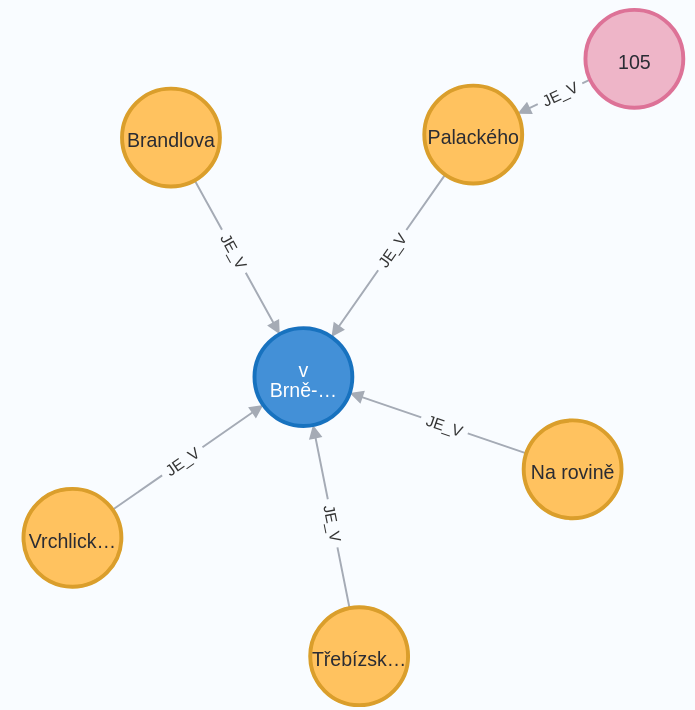
\includegraphics[width=0.8\textwidth]{obrazky-figures/adresses.png}
    \caption{Ukážka štruktúry uzlov adries}
    \label{adress}
\end{figure}

Na obrázku \ref{adress} môžeme vidieť jednoduchý demonštračný príklad. Modrý uzol reprezentuje mesto alebo dedinu, oranžový uzol ulicu a ružový uzol popisné číslo. Uzly sú následne hierarchicky prepojené podľa príslušnosti vzťahom \textit{JE\_V}. Ak by sme v databáze mali uloženú nasledujúcu štruktúru dát mesta a adries v ňom a pri spracovávaní osoby by sme sa dostali ku adrese osoby (objekt typu \textit{Domicile}), musel by byť opäť vykonaný dotaz nad databázou, aby sme zistili, či takáto adresa už v databáze existuje a následne v prípade, že už existuje, osobu prepojiť na túto adresu. V opačnom prípade by musel byť ešte aj vytvorený nový uzol pre novú adresu, opäť v reálnom čase nad databázou.

\subsubsection{Pridanie modulu data\_representation.py}

Pridávanie reprezentácie vzťahov a všetkých uzlov vo výslednej databáze si rozoberieme hierarchicky, to znamená, že začneme uzlom záznamu, ktorý nesie aj informáciu o matrike z ktorej pochádza, následne si prejdeme reprezentáciu osôb a na záver si ukážeme ako budú reprezentované uzly adries. Ešte predtým si musíme vytvoriť jednoduchý spôsob prístupu ku všetkým objektom a ich vzťahom. Preto som vytvoril nový modul implementujúci triedu \textit{DataRepresentation}. Tá bude tvoriť už spomínanú medzivrstvu pred ukladaním dát do grafovej databázy. Bude obsahovať objekty reprezentujúce všetky uzly, ich vzťahy a všetky potrebné metódy pre operácie, ktoré bude nutné vykonávať nad touto vzniknutou štruktúrou. V module \textit{create\_database.py} si potom iba vytvoríme novú inštanciu tohoto objektu a tak budeme môcť jednoducho pristupovať ku všetkým dátam a metódam. Dá sa povedať, že tento modul implementuje funkcionality, ktoré boli vykonávané v module \textit{graph\_database.py} priamo nad databázou, ale vykonáva ich nad navrhnutou reprezentáciou dát.

\subsubsection{Reprezentácia dát pomocou objektov}

Keďže potrebujeme reprezentovať veľké množstvo uzlov, bude najvhodnejšie uchovávať ich v objekte typu list z jazyku python. Takto môžeme vyriešiť ukladanie samotných objektov. Spôsob ukladania jednotlivých vzťahov sa bude pri každom type vzťahov trochu líšiť preto si o nich povieme, až keď sa dostaneme ku danému vzťahu. Objekty budú teda uložené ako atribúty v novej vzniknutej triede \textit{DataRepresentation} a budú mať formu listu. Ak teda začneme hierarchycky samotnými záznamami, tie sú reprezentované objektom \textit{Record}. Preto bude vhodné vytvoriť list všetkých objektov záznamov. Pri kažom spracovávanom zázname si teda daný záznam uložíme do tohto listu. Ďalej nasleduje objekt reprezentujúci matriku. Tým je objekt implementovaný triedou \textit{Register}. Tu budeme opakovať rovnaký postup a opäť vytvoríme list všetkých týchto objektov. Tak ako v pôvodnej implementácii bude ale nutné kontrolovať, či sa už matrika záznamu v liste nenachádza. Špeciálnu reprezentáciu vzťahu, ktorý medzi sebou má matrika a záznam matriky teda už nemusíme pridávať, keďže záznam má ako jeden zo svojich atribútov ID matriky, z ktorej pochádza. Preto ho budeme vedieť vo výsledku jednoducho prepojiť na správnu matriku z listu matrík. Príklad štruktúry databázy, ktorú sme takto práve implementovali môžeme vidieť na obrázku \ref{matrika}. Na ňom môžeme vidieť hnedý uzol reprezentujúci matriku a červené uzly reprezentujúce záznamy z matriky, ktoré sú na matriku prepojené vzťahom \textit{JE\_V}.

\begin{figure}[H]
    \centering
    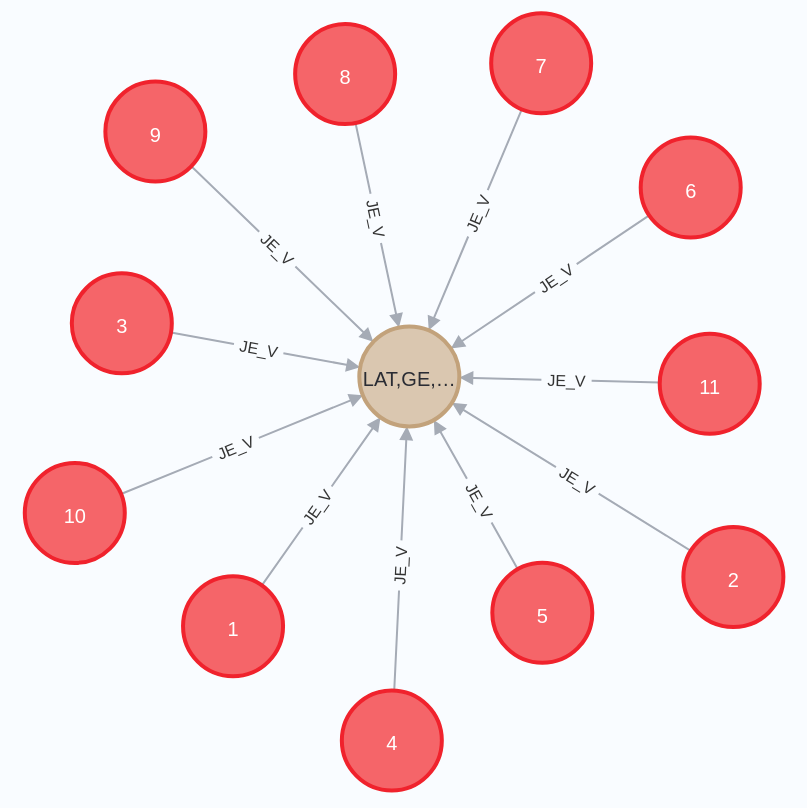
\includegraphics[width=0.8\textwidth]{obrazky-figures/matrika.png}
    \caption{Výsledná štruktúra záznamov prepojených na matriku}
    \label{matrika}
\end{figure}

Najnáročnejšou časťou bolo implementovať reprezentáciu prepojení osôb s inými osobami a osôb so záznamami. Pre reprezentovanie vzťahov osôb som sa rozhodol vytvoriť nové atribúty objektu \textit{Person}. Tento objekt po novom obsahuje atribút vo forme listu pre reprezentovanie všetkých vzťahov vedúcich z osoby (či už na iné osoby alebo na záznamy) okrem vzťahov potencionálnych zhôd, ktoré sú uložené v osobitnom liste. Okrem toho bolo nutné vedieť aj všetky vzťahy vedúce do uzla osoby, preto som vytvoril ďalší atribút typu list, ktorý uchováva aj tieto vzťahy.

Ďalšími uzlami a vzťahmi, ktoré bolo nutné uchovať sú mestá, ulice a popisné čísla. Pri spracovávaní osoby máme v už spomínanom objekte \textit{Domicile} informácie o adrese osoby. Bude preto nutné na základe informácií obsiahnutých v tomto objekte vytvárať novú štruktúru. Opäť bude vhodné pre uchovanie všetkých objektov miest vytvoriť v triede \textit{DataRepresentation} atribút typu list, do ktorého budú všetky objekty miest ukladané. 

\subsection{Štruktúra pre reprezentovanie vzťahov}

Teraz keď už vieme, kde si budeme vzťahy uchovávať, je nutné navrhnúť štruktúru pre reprezentovanie každého typu vzťahu. Toto budú štruktúry uložené v spomínaných listoch. Ako najlepší spôsob pre reprezentáciu vzťahu sa ukázal byť python objekt typu slovník. Ten uchováva dáta v pároch formou kľúčov, ku ktorým prislúchajú hodnoty.
Takým spôsobom si môžeme uchovať všetky atribúty vzťahov a zároveň reprezentovať smer vzťahov a aj sa odkazovať na uzol na ktorý vzťah smeruje. Smer vzťahov je implicitne vždy smerujúci z uzla okrem prípadu už spomínaného listu s všetkými vzťahmi smerujúcimi do uzla. Pre určenie uzla, s ktorým je pôvodný uzol (reprezentovaný objektom) vo vzťahu, používame referenciu na objekt reprezentujúci cieľový uzol. To v praxi v podstate znamená jednoduché priradenie objektu, keďže v jazyku python je priraďovanie každej hodnoty iba vytvorenie premennej odkazujúcej na rovnaký objekt.

\subsubsection{Vzťahy medzi osobami}

Na obrázku \ref{relationship} môžeme vidieť príklad vzniknutého vzťahu osoby. V tomto prípade sa jedná o vzťah medzi dvoma osobami. Slovník tvoriaci takýto vzťah sa skladá z dvoch kľúčov. Tými sú \textit{type}, ktorého hodnotou je názov vzťahu, ktorý budeme vkladať do databázy, v tomto konkrétnom príklade je to vzťah \textit{JE\_OTEC}. Ďalším kľúčom je \textit{person}, ktorého hodnotou je už samotný odkaz na objekt reprezentujúci cieľový uzol, v tomto prípade by išlo o dieťa osoby. Zakaždým, keď vytvárame takýto vzťah, je vytvorený aj vzťah v liste vzťahov smerujúcich do uzla osoby v atribúte objektu reprezentujúceho cieľový uzol. Takýto vzťah bude mať rovnakú hodnotu kľúča \textit{type} a hodnotou kľúča \textit{person} bude osoba, z ktorej vzťah smeruje. Pre uloženie vzťahov potencionálnych zhôd je potom použitý osobitný atribút. Pri reprezentácii vzťahov je v prípade potencionálnej zhody prítomný aj kľúč s porovnávacím skóre osôb.

\begin{figure}[H]
    \centering
    \begin{lstlisting}[language=python]
                        {
                          "type": "JE_OTEC",
                          "person": person_variable
                        }              
    \end{lstlisting}
    \caption{Slovník reprezentujúci vzťah osoby s inou osobou}
    \label{relationship}
\end{figure}

\subsubsection{Vzťah medzi osobou a záznamom}

Ďalším typom vzťahov, ktoré môže osoba mať sú vzťahy ku záznamom. V týchto vzťahoch potrebujeme ukladať opäť typ vzťahu, objekt na ktorý sa vzťahom odkazujeme a k tomu ešte aj dátum vytvorenia záznamu. Na obrázku \ref{relationship-record} môžeme vidieť štruktúru slovníka reprezentujúceho takýto vzťah. Opäť je tu kľúč \textit{type}, ktorého hodnotou je názov vzťahu. Ďalej tu máme kľúč \textit{record}, ktorého hodnota je odkaz na samotný objekt reprezentujúci záznam. Potom je tu ešte kľúč \textit{date}, ktorého hodnota je objekt triedy \textit{datetime.datetime} reprezentujúci dátum záznamu.

\begin{figure}[H]
    \centering
    \begin{lstlisting}[language=python]
                        {
                          "type": "OTEC",
                          "record": record_variable,
                          "date": date
                        }              
    \end{lstlisting}
    \caption{Slovník reprezentujúci vzťah osoby so záznamom}
    \label{relationship-record}
\end{figure}
\pagebreak

Na obrázku \ref{people} môžeme vidieť, akú štruktúru dát sme vytvorenými vzťahmi dokázali reprezentovať. Ide o príklad záznamu o krste a všetkých osôb, ktoré v ňom figurujú vrátane všetkých vzťahov medzi osobami a osobami a záznamom. Červený uzol tu reprezentuje záznam o krste a zelené uzly reprezentujú osoby figurujúce v zázname.

\begin{figure}[H]
    \centering
    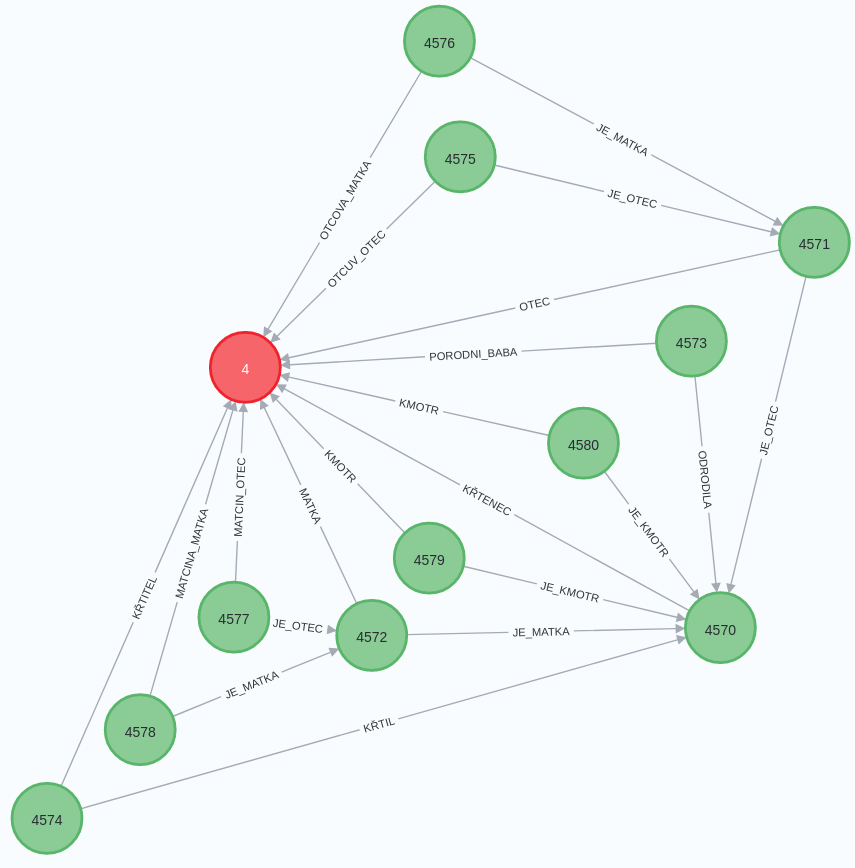
\includegraphics[width=0.8\textwidth]{obrazky-figures/people.png}
    \caption{Príklad osôb a ich vzťahov v databáze}
    \label{people}
\end{figure}

\subsubsection{Vzťah medzi osobou a uzlom adresy}

Tento typ vzťahu nebolo nutné reprezentovať novou štruktúrou, keďže každý objekt \textit{Person} už má atribút typu list objektov typu \textit{Domicile}, ktorý nám hovorí na akých adresách osoba počas života bývala. Jediné čo bolo nutné v tomto atribúte modifikovať bolo pridanie špecifického ID k atribútu ulice a popisného čísla. Toto bolo vykonané z implementačných dôvodov pri vytváraní štruktúr reprezentujúcich hierarchiu vzťahov medzi uzlami adries (teda mestami, ulicami a popisnými číslami). Keďže sme prestali robiť neustále dotazy na adresy v databáze, stratili sme informácie o existujúcich mestách a ulicách a popisných číslach v nich. To ako sme si tieto vzťahy reprezentovali si popíšeme v ďalšej sekcii. Vzťahy osôb k najdetailnejšiemu uzlu adresy (teda vzťahy \textit{BÝVA}) si vieme prepojiť jednoducho podľa atribútu s adresami osoby.

\subsection{Hierarchia vzťahov uzlov adries}

Ako už vieme, adresy uložené v databáze majú vlastnú hierarchiu vytvorenú na základe príslušnosti ulíc mestám a popisných čísel uliciam, či prípadne dedinám. Keďže sú všetky mestá uložené v liste v atribúte triedy \textit{DataRepresentation} bolo ideálne ukladať celú hierarchiu týchto vzťahov do štruktúry reprezentujúcej mesto. Najlepšou štruktúrou pre uloženie mesta a jeho vzťahov sa opäť ukázal byť slovník, keďže potrebujeme ukladať viacero pomenovaných údajov s ich hodnotami a zároveň aj vzťahy mesta (teda ulice a popisné čísla prepojené na mesto).

\lstset{
    inputencoding=utf8,
    extendedchars=true,
    literate=%
    {á}{{\'a}}1
    {č}{{\v{c}}}1
    {ď}{{\v{d}}}1
    {é}{{\'e}}1
    {ě}{{\v{e}}}1
    {í}{{\'i}}1
    {ň}{{\v{n}}}1
    {ó}{{\'o}}1
    {ř}{{\v{r}}}1
    {š}{{\v{s}}}1
    {ť}{{\v{t}}}1
    {ú}{{\'u}}1
    {ů}{{\r{u}}}1
    {ý}{{\'y}}1
    {ž}{{\v{z}}}1
    {Á}{{\'A}}1
    {Č}{{\v{C}}}1
    {Ď}{{\v{D}}}1
    {É}{{\'E}}1
    {Ě}{{\v{E}}}1
    {Í}{{\'I}}1
    {Ň}{{\v{N}}}1
    {Ó}{{\'O}}1
    {Ř}{{\v{R}}}1
    {Š}{{\v{S}}}1
    {Ť}{{\v{T}}}1
    {Ú}{{\'U}}1
    {Ů}{{\r{U}}}1
    {Ý}{{\'Y}}1
    {Ž}{{\v{Z}}}1
}

\begin{figure}[H]
    \centering
    \begin{lstlisting}[language=python]
{
  "id": uuid.uuid4(),
  "name": "V Brně-Husovicích",
  "normalized_name": None,
  "gps": [0.0,0.0]
  "streets": [
		{
		  "street_name": ("Palackého", uuid.uuid4()),
		  "numbers": [
			     	("105", uuid.uuid4())
			      ]
		},
		{
		  "street_name": ("Na rovině", uuid.uuid4()),
		  "numbers": []
		},
		{
		  "street_name": ("Brandlova", uuid.uuid4()),
		  "numbers": []
		},
		{
		  "street_name": ("Třebízského", uuid.uuid4()),
		  "numbers": []
		},
		{
		  "street_name": ("Vrchlického", uuid.uuid4()),
		  "numbers": []
		}
	     ],
  "numbers": []
}
    \end{lstlisting}
    \caption{Príklad slovníka reprezentujúceho mesto a jeho ulice a popisné čísla}
    \label{townstruct}
\end{figure}

Na obrázku \ref{townstruct} môžeme vidieť vzniknutú štruktúru mesta, ktorá reprezentuje všetky uzly a vzťahy, ktoré môžeme vidieť na obrázku \ref{adress}. Mesto je teda reprezentované slovníkom, ktorého kľúče \textit{id}, \textit{name}, \textit{normalized\_name} reprezentujú ID mesta, jeho názov a aj jeho normalizovaný názov v tomto poradí, následne je tu kľúč \textit{gps}, ktorý reprezentuje gps súradnice mesta (v prípade, že sme nenašli hodnotu súradníc získavanú zo súborov JSON, je predvolená hodnota [0.0,0.0]), kľúč \textit{streets}, ktorého hodnotou je list slovníkov reprezentujúcich ulice mesta a posledným kľúčom slovníka mesta je kľúč \textit{numbers}, ktorého hodnotou je zasa list všetkých objektov typu tuple, reprezentujúcich jednotlivé popisné čísla v meste (v prípade, že by sa jednalo o dedinu, alebo v prípade, že by chýbal údaj o ulici, do ktorej popisné číslo patrí).

Pri štruktúre reprezentujúcej ulicu sa jedná opäť o slovník, ktorého kľúče sú \textit{street\_name} a \textit{numbers}. Ich hodnotou je objekt typu tuple jednoznačne identifikujúci ulicu a list objektov typu tuple reprezentujúcich popisné čísla v tomto poradí. Objekt typu tuple reprezentujúci ulicu sa skladá z názvu ulice vo forme reťazca a z ID ulice, ktoré jednoznačne ulicu identifikuje. Pri objekte typu tuple reprezentujúcom popisné čísla ide o presne rovnaký formát dát, číže popisné číslo vo forme reťazca a id. Pre vytvorenie hodnôt ID bola použitá funkcia modulu \textit{uuid}, \textit{uuid4()}, ktorá vygeneruje náhodné ID.

\subsubsection{Vytváranie štruktúry}

Štruktúra miest v takejto podobe vzniká pri spracovaní adries spracovávanej osoby. Pre každú adresu z listu adries osoby je zavolaná funkcia \textit{create\_domicile} modulu \textit{DataRepresentation}. Tá prejde list miest a skontroluje, či sa v ňom nová adresa už nenachádza, pričom kontrola začína zhora nadol, najprv sa kontroluje, existencia mesta, potom ulíc v ňom a nakoniec aj popisných čísel. Vždy sa pridá iba potrebný najdetailnejší údaj, takže nevytvárame žiadne duplicitné mestá ani ulice.

\subsection{Výsledný algoritmus}

Vytvorenie novej podoby algoritmu ktorú som navrhol teda pozostávalo z implementácie modulu \textit{data\_representation.py} vrátane všetkých jeho metód a atribútov v podobe už spomínaných štruktúr, nahradenia všetkých volaní funkcií modulu \textit{graph\_database.py} volaniami funkcií modulu \textit{data\_representation.py}, vykonávajúcich ekvivalentné operácia nad mnou navrhnutými datovými štruktúrami a následným vložením celej výslednej štruktúry uloženej v objektoch do grafovej databázy Neo4j. Týmto spôsobom sme eliminovali a nahradili všetky časti pôvodného algoritmu, ktoré sme si vytýčili v jeho návrhu.


\section{Nové formy vstupných dát}

V tejto podkapitole si rozoberieme proces pridávania nových vstupných dát v podobe matrík úmrtí a matrík sobášov. Pozrieme sa na jednotlivé časti algoritmu, ktoré museli byť modifikované a na nové funkcionality, ktoré museli byť implementované.

\subsection{Úpravy pri zmene relačnej databázy}

Ešte pred začiatkom pridávania podpory pre nové vstupné dáta bolo nutné zmeniť spôsob, akým sa z databázy načítavajú dátumy. V pôvodnej databáze perun nebolo nutné prevádzať dátumy z reťazcov na \textit{datetime.datetime} objekty. Túto konverziu bolo nutné pridať pri každom načítanom dátume do modulu zodpovedného za načítanie dát, teda \textit{relational\_database\_birth.py}. Taktiež formát dátumov v databáze bol často nekonzistentný, s chýbajúcimi údajmi o mesiacoch či dňoch a niekedy aj rokoch. Často sa v hodnotách vyskytovali neexistujúce dni v mesiaci ako napríklad 31.9 alebo 30.2. To vždy spôsobovalo spadnutie programu pri konverzii takéhoto reťazca na objekt typu \textit{datetime.datetime}, ktorý takéto chybné údaje nepodporuje. Na miesto som preto implementoval kontroly, ktoré prípadné chýbajúce údaje doplnia reálnymi datami. Chýbajúci deň v mesiaci je preto nastavený na prvý deň v mesiaci a chýbajúci mesiac zasa na prvý mesiac v roku. Taktiež je na mieste kontrola, či údaje o mesiaci a dni nie sú zamenené. V takom prípade sú vymenené. V budúcnosti by som odporučil vykonať opravu dát v databáze, prmárne dátumov, tak aby tam boli iba reálne a úplné hodnoty, keďze nesprávne hodnoty môžu viesť ku nekonzistenciám.

\subsection{Načítanie dát}

Do modulu načítavajúceho dáta z relačnej databázy \textit{relational\_database\_birth.py} bolo nutné pridať funkcie vykonávajúce načítanie dát z tabuliek záznamov o úmrtí a sobášov, načítanie všetkých osôb figurujúcich v danom zázname a vyplnením novovzniknutých objektov typu \textit{record} a \textit{Person} všetkými údjami získanými z databázy. Taktiež bolo nutné pridať nové funkcie pre získanie dátumu záznamu, keďže dátumy záznamov rozličného typu mali rozličné názvy stĺpcov v ktorých bol dátum uložený a v prípade chýbajúceho záznamu bolo nutné dátum získať implicitne z príslušného odpovedajúceho dátumu z tabuľky osoby, ktorá zastupovala v zázname hlavnú rolu. Objekty \textit{Person} museli byť taktiež rozšírené o nové atribúty, ktorými boli údaje v nových záznamoch. Boli nimi napríklad dátum viatika, pohrebu, sobášu, rozvodu, fakt či dieťa nebolo mrtvorodené a príčina smrti osoby.

\subsection{Odhady dátumov}

Ďalšie zmeny bolo nutné implementovať vo funkcii vykonávajúcej odhad intervalu dátumu narodenia a úmrtia osoby. Tam boli pridané nové odhady vďaka novým typom dátumov a novým rolám osôb a taktiež kontextu udaného typom záznamu. Pri určovaní odhadov bolo nutné ku existujúcim pravidlám pridať nasledujúce pravidlá.

\begin{itemize}
    \item Dátum viatika musel byť najskôr mesiac pred úmrtím osoby
    \item Dátum pohrebu musel byť najneskôr mesiac po úmrtí osoby
    \item Vek matky ženícha alebo nevesty musel byť minimálne 30 rokov a maximálne 60 rokov
    \item Vek otca ženícha alebo nevesty musel byť minimálne 30 rokov a maximálne 70 rokov
    \item Vek starých rodičov ženícha alebo nevesty musel byť minimálne 45 rokov a maximálne 85 rokov
\end{itemize}


\subsection{Modifikácia riadiaceho algoritmu}

Hlavný algoritmus riadiaci porovnávanie a načítanie záznamov bol modifiovaný tak, aby po skončení spracovávania záznamov jedného typu pokračoval záznamami ďalšieho typu. Zároveň po skončení spracovávania jedného záznamu bola pridaná kontrola na typ záznamu, podľa ktorej sa určí aká funkcia na prepojenie osôb zo záznamu bude zavolaná. Bolo teda nutné implementovať aj tieto nové funkcie, ktoré prejdú všetkými osobami záznamu a vytvoria všetky spojenia medzi osobami a záznamami, pomocou metód implementovaných v module \textit{DataRepresentation}. Nové typy záznamov pridali pomerne veľké množstvo nových rôl osôb. Nové roly pridané záznamami úmrtí sú nasledovné.
\pagebreak
\begin{multicols}{2}
\begin{itemize}
    \item ZESNULÝ
    \item SYN\_ZESNULÉHO
    \item DCERA\_ZESNULÉHO
    \item MANŽEL\_ZESNULÉHO
    \item MANŽELKA\_ZESNULÉHO
    \item POCHOVAL
    \item HROBNÍK
    \item ZAOPATŘIL
    \item ZAOPATŘOVATEL
\end{itemize}
\end{multicols}

A nakoniec roly pridané záznamami o sobášoch sú nasledovné:
\begin{multicols}{2}
    \begin{itemize}
        \item ŽENÍCH
        \item JE\_MANŽEL
        \item NEVĚSTA
        \item JE\_MANŽELKA
        \item ŽENICHUV\_OTEC
        \item ŽENICHOVA\_MATKA
        \item NEVĚSTIN\_OTEC
        \item NEVĚSTINA\_MATKA
        \item MATKA\_ŽENICHOVA\_OTCE
        \item OTEC\_ŽENICHOVA\_OTCE
        \item MATKA\_ŽENICHOVY\_MATKY
        \item OTEC\_ŽENICHOVY\_MATKY
        \item MATKA\_NEVĚSTINA\_OTCE
        \item OTEC\_NEVĚSTINA\_OTCE
        \item MATKA\_NEVĚSTINY\_MATKY
        \item OTEC\_NEVĚSTINY\_MATKY
        \item BYL\_SVĚDEK
        \item ŽENICHUV\_SVĚDEK
        \item BYLA\_DRUŽIČKOU
        \item DRUŽIČKA
        \item SVĚDEK
        \item NEVĚSTIN\_ZESNULÝ\_MANŽEL
        \item ŽENICHOVA\_ZESNULÁ\_ŽENA
        \item VDOVA\_PO
        \item VDOVEC\_PO
        \item ODDÁVAJÍCÍ
    \end{itemize}
\end{multicols}

Medzi týmito rolami sú všetky nové formy spojení osôb medzi sebou a aj osôb so záznamom. Je nutné podotknúť, že nie všetky osoby figurujúce v zázname o sobáši  musia byť nutne prepojené na hlavnú osobu figurujúcu v zázname, teda na nevestu alebo ženícha. Je tomu tak preto, aby sme sa vyhli príliš vysokému množstvu vzťahov v grafovej databáze a aby sme nestratili prehľadnosť. Preto roly svedkov a oddávajúceho kňaza nie sú prepojené na hlavné osoby. Ich príslušnosť k nim však vyplýva implicitne zo záznamu.

\subsection{Porovnávanie}

Zmeny v module realizujúcom porovnanie boli iba minimálne, išlo iba o pridanie nových atribútov osoby do zostavovaného porovnávacieho vektoru. Spôsob, akým sa tieto atribúty porovnávajú je rovnaký ako iné atribúty rovnakého typu.

\section{Implementácia nových metrík}

Toto bude iba veľmi stručná podkapitola, v ktorej si povieme akým spôsobom boli pridané nové metriky pre účel otestovania ich dopadu na efektivitu výsledného algoritmu. Funkcia implementujúca Jarovu i Jaro-Winklerovu vzdialenosť je dostupná z modulu Levenshtein, ktorý práca už používa. Otestované budú ale aj iné implementácie, a to implementácia týchto porovnávacích metrík z modulu pyjarowinkler a jellyfish.

Zmeny v implementácii sa budú týkať modulu \textit{comparator.py}, kde bude stačiť jednoducho nahradiť použitie funkcie implementujúcej Levenshteinovu vzdialenosť inou funkciou implementujúcou alternatívnu metriku. Následne sa metrika otestuje nad testovacou sadou.

\section{Nová možnosť výstupu vyhľadávacích skriptov}

V čase riešenia práce vznikla požiadavka aj na rozšírenie možnosti výstupu vyhľadávacích skriptov \textit{get\textunderscore all\textunderscore records.py}, \textit{get\textunderscore person.py} a \textit{get\textunderscore family\textunderscore tree.py}. Tie doposiaľ produkovali výstup iba v podobe textu na štandardnom výstupe. Pre zvýšenie použiteľnosti dát získaných z týchto skriptov bolo žiadúce produkovať univerzálnejší výstup. Tým bol výstup vo formáe JSON. Pre vytvorenie štruktúr bolo nutné mierne upraviť základný algoritmus týchto skriptov. Bol pridaný prepínač \textit{-j}, ktorý namiesto pôvodného výstupu v podobe textu na štandardnom výstupe produkuje text vo formáte JSON na štandardný výstup. Pri skripte \textit{get\textunderscore all\textunderscore records.py} a \textit{get\textunderscore person.py} produkujú jednoduchý JSON, kde sú informácie o osobe či záznamoch zobrazené v jednotlivých políčkach za sebou. Pri skripte \textit{get\textunderscore family\textunderscore tree.py} možno stojí za zmienku fakt, že výstup bol upravený takým spôsobom, že ku položkám v štruktúre osoby je pridaná položka s názvom \textit{matka} a \textit{otec}, ktorej hodnota je celá štruktúra osôb, ktoré majú s touto osobou rodičovský vzťah. Týmto vzniká JSON forma vývodu pre danú osobu. Pre zobrazenie potomkov platí to isté s tým, že deti osoby sú zobrazené ako hodnota položky \textit{deti}. V tej sú zaradom vypísané štruktúry všetkých osôb, ktoré sú deťmi tejto osoby.

\chapter{Testovanie}

V tejto kapitole si ukážeme jednotlivé testy, ktoré výsledný skript podstúpil a ich výsledky. V testoch zameraných na výslednú efektivitu budeme porovnávať skript vo výslednej podobe so skriptom používajúcim pôvodný algoritmus. Pri testoch metrík budeme porovnávať výsledné štatistické hodnoty jednotlivých metrík s pôvodnou Levenshteinovou vzdialenosťou.

\section{Testovanie efektivity}

V tejto podkapitole si ukážeme rozdiel v efektivite, ktorý priniesli všetky zmeny implementované touto prácou. Keďže už vieme, aká bola priemerná doba porovnávania jednej osoby v pôvodnom skripte (2,084 sekúnd), môžeme túto hodnotu porovnať s výslednou hodnotou nového skriptu, získanou rovnakým spôsobom. Celková doba trvania nového skriptu pri spracovávaní tisícich záznamov krstu z databázy demos bola 1366 sekúnd a spracovaných bolo 7933 osôb. Síce sa nejedná o úplne rovnakú testovaciu vzorku, ale ide o rovnaký typ záznamov, v ktorých je takmer rovnaký počet osôb, pričom je výsledná doba trvania aj tak vydelená počtom osôb, aby sme získali priemernú hodnotu. Táto nová hodnota je 0,172 sekúnd na osobu. Aby sme teda určili výsledné zrýchlenie, môžeme vydeliť pôvodnú priemernú hodnotu porovnávania jednej osoby s novou priemernou hodnotou porovnávania. Takto nám vychádza, že je výsledný algoritmus vyše 12-krát rýchlejší.

\section{Testovanie nových metrík}

Ako prvé sa pozrieme na výsledky skriptu nad dodanou testovacou sadou, v podobe csv súborov. Pre účely porovnania metrík použijeme záznamy o krste, konkrétne pôjde o testovaciu sadu s 482 záznamami, vktorých figurujú osoby otca, matky a dieťaťa, pričom bol použitý prah dosahujúci najlepšie výsledky v základnej implementácii používajúcej Levenshteinovu vzdialenosť. Horná hodnota prahu bola 0,95 a spodná hodnota prahu bola 0,8. V nasledujúcej tabuľke môžeme vidieť prehľad jednotlivých metrík a výsledky štatistických hodnôt, ktoré dosahujú.
\pagebreak

\begin{table}[H]
\caption{Prehľad štatistických výsledkov metrík} \label{tab:results}
\begin{tabular}{ |c|c|c|c| } 
 \hline
 Použitá metrika & Precision & Recall & F-measure \\ 
 \hline
 Levenshteinova vzdialenosť & 0,775 & 0,964 & 0,859 \\
 \hline
 Jarova vzdialenosť (Levenshtein) & 0,543 & 0,986 & 0,700 \\
 \hline
 Jarova vzdialenosť (pyjarowinkler) & 0.542 & 0.987 & 0.700\\
 \hline
 Jarova vzdialenosť (jellyfish) & 0,543 & 0,987 & 0,701 \\
 \hline
 Jaro-Winklerova vzdialenosť (Levenshtein) & 0,543 & 0,987 & 0,701 \\
 \hline
 Jaro-Winklerova vzdialenosť (pyjarowinkler) & 0.542 & 0.987 & 0.700\\
 \hline
 Jaro-Winklerova vzdialenosť (jellyfish) & 0.543 & 0.987 & 0.701\\
 \hline
\end{tabular}
\end{table}

Na tabuľke \ref{tab:results} môžeme vidieť, že jednotlivé implementácie metrík sa skoro vôbec nelíšia. Zároveň môžeme pozorovať, že nové alternatívne metriky produkujú horšie štatistické výsledky pri testovacom porovnaní, rozdiel je hlavne viditelný pri presnosti, teda pomere správne identifikovaných zhôd ku všetkým identifikovaným zhodám.

\section{Vplyv nových záznamov na presnosť}

Kvôli veľkému rozdielu v počtoch pozitívnych porovnaní a negatívnych porovnaní, ktoré skript učiní, je vhodné použiť štatistickú metriku, ktorá tento fakt zohľadnuje. Tou je balancovaná presnosť (anglicky balanced accuracy) \cite{balanced}. Tá sa počíta ako priemer pomeru správne identifikovaných zhôd ku všetkým zhodám a pomeru správne identifikovaných nezhôd ku všetkým nezhodám. Takýto výsledok pre nás má výpovednú hodnotu, pretože zohľadnuje nepomer v počte týchto dvoch tried.

\begin{table}[H]
\caption{Prehľad štatistických výsledkov metrík} \label{tab:results2}
\begin{tabular}{ |c|c|c|c|c| } 
 \hline
 Typ záznamov & Precision & Recall & F-measure & Balanced accuracy \\ 
 \hline
 Iba záznamy krstov & 0.855 & 0.537 & 0.660 & 0.768 \\
 \hline
 Iba záznamy úmrtí & 0.684 & 0.786 & 0.732 & 0.890 \\
 \hline
 Iba záznamy sobášov & 0.634 & 0.675 & 0.655 & 0.836 \\
 \hline
 Všetky typy záznamov & 0.814 & 0.475 & 0.600 & 0.737\\
 \hline
\end{tabular}
\end{table}

V tabuľke \ref{tab:results2} môžeme vidieť výsledné hodnoty štatistických údajov podľa typu vstupných záznamov. Hodnoty prahov použitých pre tento test boli 0,90 pre horný a 0,7 pre spodný. Pri použití všetkých typov záznamov pozorujeme mierny pokles v štatistických hodnotách presnosti algoritmu, okrem hodnoty \textit{precision}. Horšie výsledky algoritmu môžu byť spôsobené i faktom, že vstupné testovacie dáta nie sú v normalizovanej podobe. Množstvo údajov je napísaných v rozličných variantách toho istého slova. Časté sú aj skrátené formy mien, kde je v stĺpci mena alebo priezviska uvedená skratka alebo skrátená forma mena a zároveň aj celé meno osoby. To môže negatívne ovplyvniť porovnávanie, ale poskytuje nám to pohľad ako úspešný by bol algoritmus pri spracovávaní dát v takej forme, v akej ich nájdeme priamo v matrikách (nenormalizovanej). Ďalším faktom, ktorý je nutné zohľadniť je, že množstvo osôb v porovnávacej sade nemalo priradené ID (bolo neznáme), a teda porovnania s osobami, ktoré ID nemali, nemali na štatistické výsledky skriptu žiaden vplyv, okrem faktu, že pri zjednotení s osobami, ktoré ID priradené mali, došlo ku aktualizácii hodnôt a prípadnému prehodnoteniu vzťahov danej osoby.

\chapter{Záver}

Cieľom práce bolo rozšíriť prácu Ing. Tušimovej o nové typy genealogických záznamov, zvýšiť časovú efektivitu skriptu pri použití nad databázou a vyskúšať nové alternatívy ku pôvodnej metrike, ktorú skript používal. Začiatku vypracovávania práce predchádzalo naštudovanie oboru genealógie a samotnej implementácie od Ing. Tušimovej. Nové typy záznamov boli úspešne pridané a skript vo výsledku zvládne spracovať všetky typy matričných záznamov, oproti pôvodnej verzii, ktorá fungovala iba so záznamami o krste. Efektivita skriptu pri použití nad databázou bola vo výsledku zvýšená viac ako dvanásťnásobne, ako je možné vidieť v sekcii s testovaním. Podarilo sa nám zistiť, že použitie nových metrík, konkrétne Jarovej a Jaro-Winklerovej vzdialenosti vedie ku zhoršeným výsledkom porovnávania skriptu. Ďalej sme si ukázali nedostatky práce a rôzne implementačné problémy a ich riešenia.

Vývoj práce by mohol pokračovať ďalej, bolo by možné implementovať grafické rozhranie pre vyhľadávacie skripty, pridať podporu pre ďalšie formy historických záznamov ako napríklad sčítania ľudi, či vyskúšať alternatívy ku metódam použitým v procese porovnávania.
%===============================================================================

  \fi
  
  % Kompilace po částech (viz výše, nutno odkomentovat)
  % Compilation piecewise (see above, it is necessary to uncomment it)
  %\subfile{projekt-01-uvod-introduction}
  % ...
  %\subfile{chapters/projekt-05-conclusion}


  % Pouzita literatura / Bibliography
  % ----------------------------------------------
\ifslovak
  \makeatletter
  \def\@openbib@code{\addcontentsline{toc}{chapter}{Literatúra}}
  \makeatother
  \bibliographystyle{bib-styles/Pysny/skplain}
\else
  \ifczech
    \makeatletter
    \def\@openbib@code{\addcontentsline{toc}{chapter}{Literatura}}
    \makeatother
    \bibliographystyle{bib-styles/Pysny/czplain}
  \else 
    \makeatletter
    \def\@openbib@code{\addcontentsline{toc}{chapter}{Bibliography}}
    \makeatother
    \bibliographystyle{bib-styles/Pysny/enplain}
  %  \bibliographystyle{alpha}
  \fi
\fi
  \begin{flushleft}
  \bibliography{projekt-20-literatura-bibliography}
  \end{flushleft}

  % vynechani stranky v oboustrannem rezimu
  % Skip the page in the two-sided mode
  \iftwoside
    \cleardoublepage
  \fi

  % Prilohy / Appendices
  % ---------------------------------------------
  \appendix
\ifczech
  \renewcommand{\appendixpagename}{Přílohy}
  \renewcommand{\appendixtocname}{Přílohy}
  \renewcommand{\appendixname}{Příloha}
\fi
\ifslovak
  \renewcommand{\appendixpagename}{Prílohy}
  \renewcommand{\appendixtocname}{Prílohy}
  \renewcommand{\appendixname}{Príloha}
\fi
%  \appendixpage

% vynechani stranky v oboustrannem rezimu
% Skip the page in the two-sided mode
%\iftwoside
%  \cleardoublepage
%\fi
  
\ifslovak
%  \section*{Zoznam príloh}
%  \addcontentsline{toc}{section}{Zoznam príloh}
\else
  \ifczech
%    \section*{Seznam příloh}
%    \addcontentsline{toc}{section}{Seznam příloh}
  \else
%    \section*{List of Appendices}
%    \addcontentsline{toc}{section}{List of Appendices}
  \fi
\fi
  \startcontents[chapters]
  \setlength{\parskip}{0pt} 
  % seznam příloh / list of appendices
  % \printcontents[chapters]{l}{0}{\setcounter{tocdepth}{2}}
  
  \ifODSAZ
    \setlength{\parskip}{0.5\bigskipamount}
  \else
    \setlength{\parskip}{0pt}
  \fi
  
  % vynechani stranky v oboustrannem rezimu
  \iftwoside
    \cleardoublepage
  \fi
  
  % Přílohy / Appendices

  
  % Kompilace po částech (viz výše, nutno odkomentovat)
  % Compilation piecewise (see above, it is necessary to uncomment it)
  %\subfile{projekt-30-prilohy-appendices}
  
\end{document}
